\documentclass[twoside]{book}

% Packages required by doxygen
\usepackage{fixltx2e}
\usepackage{calc}
\usepackage{doxygen}
\usepackage[export]{adjustbox} % also loads graphicx
\usepackage{graphicx}
\usepackage[utf8]{inputenc}
\usepackage{makeidx}
\usepackage{multicol}
\usepackage{multirow}
\PassOptionsToPackage{warn}{textcomp}
\usepackage{textcomp}
\usepackage[nointegrals]{wasysym}
\usepackage[table]{xcolor}

% NLS support packages
\usepackage[french]{babel}

% Font selection
\usepackage[T1]{fontenc}
\usepackage[scaled=.90]{helvet}
\usepackage{courier}
\usepackage{amssymb}
\usepackage{sectsty}
\renewcommand{\familydefault}{\sfdefault}
\allsectionsfont{%
  \fontseries{bc}\selectfont%
  \color{darkgray}%
}
\renewcommand{\DoxyLabelFont}{%
  \fontseries{bc}\selectfont%
  \color{darkgray}%
}
\newcommand{\+}{\discretionary{\mbox{\scriptsize$\hookleftarrow$}}{}{}}

% Page & text layout
\usepackage{geometry}
\geometry{%
  a4paper,%
  top=2.5cm,%
  bottom=2.5cm,%
  left=2.5cm,%
  right=2.5cm%
}
\tolerance=750
\hfuzz=15pt
\hbadness=750
\setlength{\emergencystretch}{15pt}
\setlength{\parindent}{0cm}
\setlength{\parskip}{3ex plus 2ex minus 2ex}
\makeatletter
\renewcommand{\paragraph}{%
  \@startsection{paragraph}{4}{0ex}{-1.0ex}{1.0ex}{%
    \normalfont\normalsize\bfseries\SS@parafont%
  }%
}
\renewcommand{\subparagraph}{%
  \@startsection{subparagraph}{5}{0ex}{-1.0ex}{1.0ex}{%
    \normalfont\normalsize\bfseries\SS@subparafont%
  }%
}
\makeatother

% Headers & footers
\usepackage{fancyhdr}
\pagestyle{fancyplain}
\fancyhead[LE]{\fancyplain{}{\bfseries\thepage}}
\fancyhead[CE]{\fancyplain{}{}}
\fancyhead[RE]{\fancyplain{}{\bfseries\leftmark}}
\fancyhead[LO]{\fancyplain{}{\bfseries\rightmark}}
\fancyhead[CO]{\fancyplain{}{}}
\fancyhead[RO]{\fancyplain{}{\bfseries\thepage}}
\fancyfoot[LE]{\fancyplain{}{}}
\fancyfoot[CE]{\fancyplain{}{}}
\fancyfoot[RE]{\fancyplain{}{\bfseries\scriptsize Généré par Doxygen }}
\fancyfoot[LO]{\fancyplain{}{\bfseries\scriptsize Généré par Doxygen }}
\fancyfoot[CO]{\fancyplain{}{}}
\fancyfoot[RO]{\fancyplain{}{}}
\renewcommand{\footrulewidth}{0.4pt}
\renewcommand{\chaptermark}[1]{%
  \markboth{#1}{}%
}
\renewcommand{\sectionmark}[1]{%
  \markright{\thesection\ #1}%
}

% Indices & bibliography
\usepackage{natbib}
\usepackage[titles]{tocloft}
\setcounter{tocdepth}{3}
\setcounter{secnumdepth}{5}
\makeindex

% Hyperlinks (required, but should be loaded last)
\usepackage{ifpdf}
\ifpdf
  \usepackage[pdftex,pagebackref=true]{hyperref}
\else
  \usepackage[ps2pdf,pagebackref=true]{hyperref}
\fi
\hypersetup{%
  colorlinks=true,%
  linkcolor=blue,%
  citecolor=blue,%
  unicode%
}

% Custom commands
\newcommand{\clearemptydoublepage}{%
  \newpage{\pagestyle{empty}\cleardoublepage}%
}

\usepackage{caption}
\captionsetup{labelsep=space,justification=centering,font={bf},singlelinecheck=off,skip=4pt,position=top}

%===== C O N T E N T S =====

\begin{document}

% Titlepage & ToC
\hypersetup{pageanchor=false,
             bookmarksnumbered=true,
             pdfencoding=unicode
            }
\pagenumbering{alph}
\begin{titlepage}
\vspace*{7cm}
\begin{center}%
{\Large Projet L2 Informatique -\/ The Hive }\\
\vspace*{1cm}
{\large Généré par Doxygen 1.8.13}\\
\end{center}
\end{titlepage}
\clearemptydoublepage
\pagenumbering{roman}
\tableofcontents
\clearemptydoublepage
\pagenumbering{arabic}
\hypersetup{pageanchor=true}

%--- Begin generated contents ---
\chapter{Index des fichiers}
\section{Liste des fichiers}
Liste de tous les fichiers documentés avec une brève description \+:\begin{DoxyCompactList}
\item\contentsline{section}{src/\hyperlink{backup__and__load_8c}{backup\+\_\+and\+\_\+load.\+c} \\*Sauvegarde et chargement d\textquotesingle{}une partie }{\pageref{backup__and__load_8c}}{}
\item\contentsline{section}{src/\hyperlink{eat__or__drink_8c}{eat\+\_\+or\+\_\+drink.\+c} \\*Fonctionnalité \+: manger ou boire un item de son inventaire }{\pageref{eat__or__drink_8c}}{}
\item\contentsline{section}{src/\hyperlink{equipment_8c}{equipment.\+c} \\*Gestion de l\textquotesingle{}équipement du joueur }{\pageref{equipment_8c}}{}
\item\contentsline{section}{src/\hyperlink{exit__help_8c}{exit\+\_\+help.\+c} \\*Sortie + Aide }{\pageref{exit__help_8c}}{}
\item\contentsline{section}{src/\hyperlink{fish_8c}{fish.\+c} \\*Fonctionnalité \+: pêcher }{\pageref{fish_8c}}{}
\item\contentsline{section}{src/\hyperlink{inventory_8c}{inventory.\+c} \\*Gestion de l\textquotesingle{}inventaire du joueur }{\pageref{inventory_8c}}{}
\item\contentsline{section}{src/\hyperlink{items_8c}{items.\+c} \\*Fonctions relatives aux items }{\pageref{items_8c}}{}
\item\contentsline{section}{src/\hyperlink{menu_8c}{menu.\+c} \\*M\+E\+NU P\+R\+I\+N\+C\+I\+P\+AL }{\pageref{menu_8c}}{}
\item\contentsline{section}{src/\hyperlink{move_8c}{move.\+c} \\*Gestion du déplacement du joueur }{\pageref{move_8c}}{}
\item\contentsline{section}{src/\hyperlink{perso_8c}{perso.\+c} \\*Fonctions relatives au joueur }{\pageref{perso_8c}}{}
\item\contentsline{section}{src/\hyperlink{quete__soin_8c}{quete\+\_\+soin.\+c} \\*Fonctions utilisees dans la quete \char`\"{}soin\char`\"{} }{\pageref{quete__soin_8c}}{}
\item\contentsline{section}{src/\hyperlink{quetes_8c}{quetes.\+c} \\*Fonctionalite \+: Actionner quetes du jeu }{\pageref{quetes_8c}}{}
\item\contentsline{section}{src/\hyperlink{scavenge_8c}{scavenge.\+c} \\*Fonctionnalité \+: fouiller l\textquotesingle{}hexagone pour récupérer des items }{\pageref{scavenge_8c}}{}
\item\contentsline{section}{src/\hyperlink{turn_8c}{turn.\+c} \\*Fonctions relatives à un tour du jeu }{\pageref{turn_8c}}{}
\item\contentsline{section}{src/\hyperlink{world__generation_8c}{world\+\_\+generation.\+c} \\*Génération de la carte (Moustapha --$>$ C\+O\+M\+P\+L\+E\+T\+ER D\+O\+C\+U\+M\+E\+N\+T\+A\+T\+I\+ON D\+ES F\+O\+N\+C\+T\+I\+O\+NS) }{\pageref{world__generation_8c}}{}
\end{DoxyCompactList}

\chapter{Documentation des fichiers}
\hypertarget{backup__and__load_8c}{}\section{Référence du fichier src/backup\+\_\+and\+\_\+load.c}
\label{backup__and__load_8c}\index{src/backup\+\_\+and\+\_\+load.\+c@{src/backup\+\_\+and\+\_\+load.\+c}}


Sauvegarde et chargement d\textquotesingle{}une partie.  


{\ttfamily \#include $<$stdio.\+h$>$}\newline
{\ttfamily \#include $<$stdlib.\+h$>$}\newline
{\ttfamily \#include $<$string.\+h$>$}\newline
{\ttfamily \#include \char`\"{}lib/structure.\+h\char`\"{}}\newline
Graphe des dépendances par inclusion de backup\+\_\+and\+\_\+load.\+c\+:\nopagebreak
\begin{figure}[H]
\begin{center}
\leavevmode
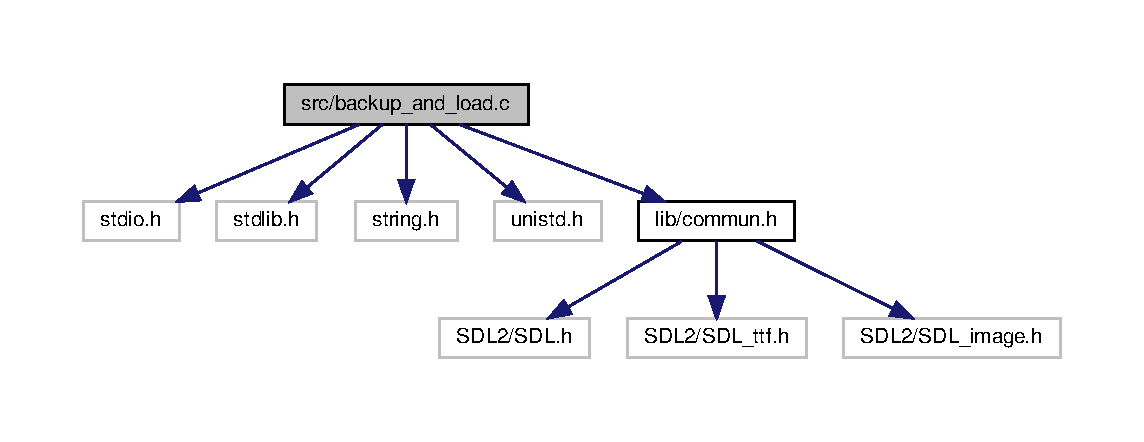
\includegraphics[width=350pt]{backup__and__load_8c__incl}
\end{center}
\end{figure}
\subsection*{Fonctions}
\begin{DoxyCompactItemize}
\item 
void \hyperlink{backup__and__load_8c_a6d4382fa7768898a8b2bce5da601bf5a}{save} (perso\+\_\+t player, cell\+\_\+t map\mbox{[}D\mbox{]}\mbox{[}D\mbox{]}, int quest\+\_\+map\mbox{[}6\mbox{]}\mbox{[}2\mbox{]}, quete\+\_\+t quete)
\begin{DoxyCompactList}\small\item\em Sauvegarde les informations sur le joueur, son inventaire, son équipement et la carte. \end{DoxyCompactList}\item 
void \hyperlink{backup__and__load_8c_ac314a90f64bb57b83647985dcba056bb}{save\+\_\+quete} (int quest\+\_\+map\mbox{[}6\mbox{]}\mbox{[}2\mbox{]}, quete\+\_\+t quete)
\begin{DoxyCompactList}\small\item\em Sauvegarde les informations sur les quêtes. \end{DoxyCompactList}\item 
void \hyperlink{backup__and__load_8c_a9411cc773bca4d1a8a475b63fdbb82b1}{save\+\_\+inventory} (perso\+\_\+t player)
\begin{DoxyCompactList}\small\item\em Sauvegarde l\textquotesingle{}inventaire du joueur dans un fichier \textquotesingle{}save\+\_\+inventory.\+csv\textquotesingle{}. \end{DoxyCompactList}\item 
void \hyperlink{backup__and__load_8c_ac7e17aee692ea956b96122bd0f8cbe2c}{save\+\_\+info\+\_\+player} (perso\+\_\+t player)
\begin{DoxyCompactList}\small\item\em Sauvegarde les informations du joueur dans un fichier \textquotesingle{}save\+\_\+info\+\_\+player. \end{DoxyCompactList}\item 
void \hyperlink{backup__and__load_8c_af29212eb7ae8429e0c6ed7b486077e28}{save\+\_\+equipment} (perso\+\_\+t player)
\begin{DoxyCompactList}\small\item\em Sauvegarde l\textquotesingle{}équipement du joueur dans un fichier \textquotesingle{}save\+\_\+equipment.\+csv\textquotesingle{}. \end{DoxyCompactList}\item 
void \hyperlink{backup__and__load_8c_a20bf83b117d4618a1cdd44f63b99ce49}{save\+\_\+map} (cell\+\_\+t map\mbox{[}D\mbox{]}\mbox{[}D\mbox{]})
\begin{DoxyCompactList}\small\item\em Sauvegarde la carte dans un fichier \textquotesingle{}save\+\_\+map.\+csv\textquotesingle{}. \end{DoxyCompactList}\item 
int \hyperlink{backup__and__load_8c_a0006d1b730137142326f7172e9ec9275}{load} (perso\+\_\+t $\ast$player, cell\+\_\+t map\mbox{[}D\mbox{]}\mbox{[}D\mbox{]}, int quest\+\_\+map\mbox{[}6\mbox{]}\mbox{[}2\mbox{]}, quete\+\_\+t $\ast$quete)
\begin{DoxyCompactList}\small\item\em Charge les informations sur le joueur, son inventaire, son équipement et la carte. \end{DoxyCompactList}\item 
int \hyperlink{backup__and__load_8c_a1ca7baefc14b21bed6f7f23cb2b81061}{load\+\_\+inventory} (perso\+\_\+t $\ast$player)
\begin{DoxyCompactList}\small\item\em Charge l\textquotesingle{}inventaire du joueur à partir du fichier \textquotesingle{}save\+\_\+inventory.\+csv\textquotesingle{}. \end{DoxyCompactList}\item 
int \hyperlink{backup__and__load_8c_a347aef6e50f726155f0ca327f3584bc1}{load\+\_\+info\+\_\+player} (perso\+\_\+t $\ast$player)
\begin{DoxyCompactList}\small\item\em Charge les informations du joueur à partir du fichier \textquotesingle{}save\+\_\+info\+\_\+player.\+csv\textquotesingle{}. \end{DoxyCompactList}\item 
int \hyperlink{backup__and__load_8c_af55f140477f851e77110b44043b15f32}{load\+\_\+equipment} (perso\+\_\+t $\ast$player)
\begin{DoxyCompactList}\small\item\em Charge l\textquotesingle{}équipement du joueur à partir du fichier \textquotesingle{}save\+\_\+equipment.\+csv\textquotesingle{}. \end{DoxyCompactList}\item 
int \hyperlink{backup__and__load_8c_aeb1455e8d9868dbe3fa2dc0df61f3ce4}{load\+\_\+map} (cell\+\_\+t map\mbox{[}D\mbox{]}\mbox{[}D\mbox{]})
\begin{DoxyCompactList}\small\item\em Charge la carte à partir du fichier \textquotesingle{}save\+\_\+map.\+csv\textquotesingle{}. \end{DoxyCompactList}\item 
int \hyperlink{backup__and__load_8c_ae070760c3aa26e4d1476f2b7d07a2b1c}{load\+\_\+quete} (int quest\+\_\+map\mbox{[}6\mbox{]}\mbox{[}2\mbox{]}, quete\+\_\+t $\ast$quete)
\begin{DoxyCompactList}\small\item\em Charge les informations des quêtes à partir du fichier \textquotesingle{}save\+\_\+quete.\+csv\textquotesingle{}. \end{DoxyCompactList}\item 
int \hyperlink{backup__and__load_8c_aab0014eee5b94780b856a7682ae49b30}{backup\+\_\+exists} ()
\begin{DoxyCompactList}\small\item\em Vérifie si une sauvegarde complète du jeu existe. \end{DoxyCompactList}\item 
int \hyperlink{backup__and__load_8c_ad5bc95791f73c2f23fbd99cdb8c7e1f2}{init\+\_\+or\+\_\+load\+\_\+game} (perso\+\_\+t $\ast$player, cell\+\_\+t map\mbox{[}D\mbox{]}\mbox{[}D\mbox{]}, int quest\+\_\+map\mbox{[}6\mbox{]}\mbox{[}2\mbox{]}, quete\+\_\+t $\ast$quete)
\begin{DoxyCompactList}\small\item\em Si une sauvegarde du jeu existe, propose au joueur de continuer la partie ou d\textquotesingle{}en commencer une nouvelle. \end{DoxyCompactList}\end{DoxyCompactItemize}


\subsection{Description détaillée}
Sauvegarde et chargement d\textquotesingle{}une partie. 

\begin{DoxyAuthor}{Auteur}
Mathilde Mottay, Anaïs Mottier, Clément Mainguy, Moustapha Tsamarayev 
\end{DoxyAuthor}
\begin{DoxyVersion}{Version}
1.\+0 
\end{DoxyVersion}
\begin{DoxyDate}{Date}
2020 
\end{DoxyDate}


\subsection{Documentation des fonctions}
\mbox{\Hypertarget{backup__and__load_8c_aab0014eee5b94780b856a7682ae49b30}\label{backup__and__load_8c_aab0014eee5b94780b856a7682ae49b30}} 
\index{backup\+\_\+and\+\_\+load.\+c@{backup\+\_\+and\+\_\+load.\+c}!backup\+\_\+exists@{backup\+\_\+exists}}
\index{backup\+\_\+exists@{backup\+\_\+exists}!backup\+\_\+and\+\_\+load.\+c@{backup\+\_\+and\+\_\+load.\+c}}
\subsubsection{\texorpdfstring{backup\+\_\+exists()}{backup\_exists()}}
{\footnotesize\ttfamily int backup\+\_\+exists (\begin{DoxyParamCaption}{ }\end{DoxyParamCaption})}



Vérifie si une sauvegarde complète du jeu existe. 

\begin{DoxyReturn}{Renvoie}
Un {\itshape int} \+: 1 si sauvegarde existante. 0 sinon. 
\end{DoxyReturn}
\mbox{\Hypertarget{backup__and__load_8c_ad5bc95791f73c2f23fbd99cdb8c7e1f2}\label{backup__and__load_8c_ad5bc95791f73c2f23fbd99cdb8c7e1f2}} 
\index{backup\+\_\+and\+\_\+load.\+c@{backup\+\_\+and\+\_\+load.\+c}!init\+\_\+or\+\_\+load\+\_\+game@{init\+\_\+or\+\_\+load\+\_\+game}}
\index{init\+\_\+or\+\_\+load\+\_\+game@{init\+\_\+or\+\_\+load\+\_\+game}!backup\+\_\+and\+\_\+load.\+c@{backup\+\_\+and\+\_\+load.\+c}}
\subsubsection{\texorpdfstring{init\+\_\+or\+\_\+load\+\_\+game()}{init\_or\_load\_game()}}
{\footnotesize\ttfamily int init\+\_\+or\+\_\+load\+\_\+game (\begin{DoxyParamCaption}\item[{perso\+\_\+t $\ast$}]{player,  }\item[{cell\+\_\+t}]{map\mbox{[}\+D\mbox{]}\mbox{[}\+D\mbox{]},  }\item[{int}]{quest\+\_\+map\mbox{[}6\mbox{]}\mbox{[}2\mbox{]},  }\item[{quete\+\_\+t $\ast$}]{quete }\end{DoxyParamCaption})}



Si une sauvegarde du jeu existe, propose au joueur de continuer la partie ou d\textquotesingle{}en commencer une nouvelle. 

Si aucune sauvegarde, initialise une nouvelle partie. 
\begin{DoxyParams}{Paramètres}
{\em perso\+\_\+t} & $\ast$ player \\
\hline
{\em cell\+\_\+t} & map\mbox{[}D\mbox{]}\mbox{[}D\mbox{]} \\
\hline
{\em int} & quest\+\_\+map\mbox{[}6\mbox{]}\mbox{[}2\mbox{]} \\
\hline
{\em quete\+\_\+t} & $\ast$ quete \\
\hline
\end{DoxyParams}
\begin{DoxyReturn}{Renvoie}
Un {\itshape int} \+: 1 si initialisation / chargement réussi. 0 si échec. 
\end{DoxyReturn}
\mbox{\Hypertarget{backup__and__load_8c_a0006d1b730137142326f7172e9ec9275}\label{backup__and__load_8c_a0006d1b730137142326f7172e9ec9275}} 
\index{backup\+\_\+and\+\_\+load.\+c@{backup\+\_\+and\+\_\+load.\+c}!load@{load}}
\index{load@{load}!backup\+\_\+and\+\_\+load.\+c@{backup\+\_\+and\+\_\+load.\+c}}
\subsubsection{\texorpdfstring{load()}{load()}}
{\footnotesize\ttfamily int load (\begin{DoxyParamCaption}\item[{perso\+\_\+t $\ast$}]{player,  }\item[{cell\+\_\+t}]{map\mbox{[}\+D\mbox{]}\mbox{[}\+D\mbox{]},  }\item[{int}]{quest\+\_\+map\mbox{[}6\mbox{]}\mbox{[}2\mbox{]},  }\item[{quete\+\_\+t $\ast$}]{quete }\end{DoxyParamCaption})}



Charge les informations sur le joueur, son inventaire, son équipement et la carte. 


\begin{DoxyParams}{Paramètres}
{\em perso\+\_\+t} & $\ast$ player \\
\hline
{\em cell\+\_\+t} & map\mbox{[}D\mbox{]}\mbox{[}D\mbox{]} \\
\hline
{\em int} & quest\+\_\+map\mbox{[}6\mbox{]}\mbox{[}2\mbox{]} \\
\hline
{\em quete\+\_\+t} & $\ast$ quete \\
\hline
\end{DoxyParams}
\begin{DoxyReturn}{Renvoie}
Un {\itshape int} \+: 1 si succès complet du chargement. 0 si problème lors du chargement. 
\end{DoxyReturn}
\mbox{\Hypertarget{backup__and__load_8c_af55f140477f851e77110b44043b15f32}\label{backup__and__load_8c_af55f140477f851e77110b44043b15f32}} 
\index{backup\+\_\+and\+\_\+load.\+c@{backup\+\_\+and\+\_\+load.\+c}!load\+\_\+equipment@{load\+\_\+equipment}}
\index{load\+\_\+equipment@{load\+\_\+equipment}!backup\+\_\+and\+\_\+load.\+c@{backup\+\_\+and\+\_\+load.\+c}}
\subsubsection{\texorpdfstring{load\+\_\+equipment()}{load\_equipment()}}
{\footnotesize\ttfamily int load\+\_\+equipment (\begin{DoxyParamCaption}\item[{perso\+\_\+t $\ast$}]{player }\end{DoxyParamCaption})}



Charge l\textquotesingle{}équipement du joueur à partir du fichier \textquotesingle{}save\+\_\+equipment.\+csv\textquotesingle{}. 


\begin{DoxyParams}{Paramètres}
{\em perso\+\_\+t} & $\ast$ player \\
\hline
\end{DoxyParams}
\begin{DoxyReturn}{Renvoie}
Un {\itshape int} \+: 1 si chargement réussi. 0 si échec du chargement. 
\end{DoxyReturn}
\mbox{\Hypertarget{backup__and__load_8c_a347aef6e50f726155f0ca327f3584bc1}\label{backup__and__load_8c_a347aef6e50f726155f0ca327f3584bc1}} 
\index{backup\+\_\+and\+\_\+load.\+c@{backup\+\_\+and\+\_\+load.\+c}!load\+\_\+info\+\_\+player@{load\+\_\+info\+\_\+player}}
\index{load\+\_\+info\+\_\+player@{load\+\_\+info\+\_\+player}!backup\+\_\+and\+\_\+load.\+c@{backup\+\_\+and\+\_\+load.\+c}}
\subsubsection{\texorpdfstring{load\+\_\+info\+\_\+player()}{load\_info\_player()}}
{\footnotesize\ttfamily int load\+\_\+info\+\_\+player (\begin{DoxyParamCaption}\item[{perso\+\_\+t $\ast$}]{player }\end{DoxyParamCaption})}



Charge les informations du joueur à partir du fichier \textquotesingle{}save\+\_\+info\+\_\+player.\+csv\textquotesingle{}. 


\begin{DoxyParams}{Paramètres}
{\em perso\+\_\+t} & $\ast$ player \\
\hline
\end{DoxyParams}
\begin{DoxyReturn}{Renvoie}
Un {\itshape int} \+: 1 si chargement réussi. 0 si échec du chargement. 
\end{DoxyReturn}
\mbox{\Hypertarget{backup__and__load_8c_a1ca7baefc14b21bed6f7f23cb2b81061}\label{backup__and__load_8c_a1ca7baefc14b21bed6f7f23cb2b81061}} 
\index{backup\+\_\+and\+\_\+load.\+c@{backup\+\_\+and\+\_\+load.\+c}!load\+\_\+inventory@{load\+\_\+inventory}}
\index{load\+\_\+inventory@{load\+\_\+inventory}!backup\+\_\+and\+\_\+load.\+c@{backup\+\_\+and\+\_\+load.\+c}}
\subsubsection{\texorpdfstring{load\+\_\+inventory()}{load\_inventory()}}
{\footnotesize\ttfamily int load\+\_\+inventory (\begin{DoxyParamCaption}\item[{perso\+\_\+t $\ast$}]{player }\end{DoxyParamCaption})}



Charge l\textquotesingle{}inventaire du joueur à partir du fichier \textquotesingle{}save\+\_\+inventory.\+csv\textquotesingle{}. 


\begin{DoxyParams}{Paramètres}
{\em perso\+\_\+t} & $\ast$ player \\
\hline
\end{DoxyParams}
\begin{DoxyReturn}{Renvoie}
Un {\itshape int} \+: 1 si chargement réussi. 0 si échec du chargement. 
\end{DoxyReturn}
\mbox{\Hypertarget{backup__and__load_8c_aeb1455e8d9868dbe3fa2dc0df61f3ce4}\label{backup__and__load_8c_aeb1455e8d9868dbe3fa2dc0df61f3ce4}} 
\index{backup\+\_\+and\+\_\+load.\+c@{backup\+\_\+and\+\_\+load.\+c}!load\+\_\+map@{load\+\_\+map}}
\index{load\+\_\+map@{load\+\_\+map}!backup\+\_\+and\+\_\+load.\+c@{backup\+\_\+and\+\_\+load.\+c}}
\subsubsection{\texorpdfstring{load\+\_\+map()}{load\_map()}}
{\footnotesize\ttfamily int load\+\_\+map (\begin{DoxyParamCaption}\item[{cell\+\_\+t}]{map\mbox{[}\+D\mbox{]}\mbox{[}\+D\mbox{]} }\end{DoxyParamCaption})}



Charge la carte à partir du fichier \textquotesingle{}save\+\_\+map.\+csv\textquotesingle{}. 


\begin{DoxyParams}{Paramètres}
{\em cell\+\_\+t} & map\mbox{[}D\mbox{]}\mbox{[}D\mbox{]} \\
\hline
\end{DoxyParams}
\begin{DoxyReturn}{Renvoie}
Un {\itshape int} \+: 1 si chargement réussi. 0 si échec du chargement. 
\end{DoxyReturn}
\mbox{\Hypertarget{backup__and__load_8c_ae070760c3aa26e4d1476f2b7d07a2b1c}\label{backup__and__load_8c_ae070760c3aa26e4d1476f2b7d07a2b1c}} 
\index{backup\+\_\+and\+\_\+load.\+c@{backup\+\_\+and\+\_\+load.\+c}!load\+\_\+quete@{load\+\_\+quete}}
\index{load\+\_\+quete@{load\+\_\+quete}!backup\+\_\+and\+\_\+load.\+c@{backup\+\_\+and\+\_\+load.\+c}}
\subsubsection{\texorpdfstring{load\+\_\+quete()}{load\_quete()}}
{\footnotesize\ttfamily int load\+\_\+quete (\begin{DoxyParamCaption}\item[{int}]{quest\+\_\+map\mbox{[}6\mbox{]}\mbox{[}2\mbox{]},  }\item[{quete\+\_\+t $\ast$}]{quete }\end{DoxyParamCaption})}



Charge les informations des quêtes à partir du fichier \textquotesingle{}save\+\_\+quete.\+csv\textquotesingle{}. 


\begin{DoxyParams}{Paramètres}
{\em int} & quest\+\_\+map\mbox{[}6\mbox{]}\mbox{[}2\mbox{]} \\
\hline
{\em quete\+\_\+t} & $\ast$ quete \\
\hline
\end{DoxyParams}
\begin{DoxyReturn}{Renvoie}
Un {\itshape int} \+: 1 si chargement réussi. 0 si échec du chargement. 
\end{DoxyReturn}
\mbox{\Hypertarget{backup__and__load_8c_a6d4382fa7768898a8b2bce5da601bf5a}\label{backup__and__load_8c_a6d4382fa7768898a8b2bce5da601bf5a}} 
\index{backup\+\_\+and\+\_\+load.\+c@{backup\+\_\+and\+\_\+load.\+c}!save@{save}}
\index{save@{save}!backup\+\_\+and\+\_\+load.\+c@{backup\+\_\+and\+\_\+load.\+c}}
\subsubsection{\texorpdfstring{save()}{save()}}
{\footnotesize\ttfamily void save (\begin{DoxyParamCaption}\item[{perso\+\_\+t}]{player,  }\item[{cell\+\_\+t}]{map\mbox{[}\+D\mbox{]}\mbox{[}\+D\mbox{]},  }\item[{int}]{quest\+\_\+map\mbox{[}6\mbox{]}\mbox{[}2\mbox{]},  }\item[{quete\+\_\+t}]{quete }\end{DoxyParamCaption})}



Sauvegarde les informations sur le joueur, son inventaire, son équipement et la carte. 


\begin{DoxyParams}{Paramètres}
{\em perso\+\_\+t} & player \\
\hline
{\em cell\+\_\+t} & map\mbox{[}D\mbox{]}\mbox{[}D\mbox{]} \\
\hline
{\em int} & quest\+\_\+map\mbox{[}6\mbox{]}\mbox{[}2\mbox{]} \\
\hline
{\em quete\+\_\+t} & quete \\
\hline
\end{DoxyParams}
\begin{DoxyReturn}{Renvoie}
Rien 
\end{DoxyReturn}
\mbox{\Hypertarget{backup__and__load_8c_af29212eb7ae8429e0c6ed7b486077e28}\label{backup__and__load_8c_af29212eb7ae8429e0c6ed7b486077e28}} 
\index{backup\+\_\+and\+\_\+load.\+c@{backup\+\_\+and\+\_\+load.\+c}!save\+\_\+equipment@{save\+\_\+equipment}}
\index{save\+\_\+equipment@{save\+\_\+equipment}!backup\+\_\+and\+\_\+load.\+c@{backup\+\_\+and\+\_\+load.\+c}}
\subsubsection{\texorpdfstring{save\+\_\+equipment()}{save\_equipment()}}
{\footnotesize\ttfamily void save\+\_\+equipment (\begin{DoxyParamCaption}\item[{perso\+\_\+t}]{player }\end{DoxyParamCaption})}



Sauvegarde l\textquotesingle{}équipement du joueur dans un fichier \textquotesingle{}save\+\_\+equipment.\+csv\textquotesingle{}. 


\begin{DoxyParams}{Paramètres}
{\em perso\+\_\+t} & player \\
\hline
\end{DoxyParams}
\begin{DoxyReturn}{Renvoie}
Rien 
\end{DoxyReturn}
\mbox{\Hypertarget{backup__and__load_8c_ac7e17aee692ea956b96122bd0f8cbe2c}\label{backup__and__load_8c_ac7e17aee692ea956b96122bd0f8cbe2c}} 
\index{backup\+\_\+and\+\_\+load.\+c@{backup\+\_\+and\+\_\+load.\+c}!save\+\_\+info\+\_\+player@{save\+\_\+info\+\_\+player}}
\index{save\+\_\+info\+\_\+player@{save\+\_\+info\+\_\+player}!backup\+\_\+and\+\_\+load.\+c@{backup\+\_\+and\+\_\+load.\+c}}
\subsubsection{\texorpdfstring{save\+\_\+info\+\_\+player()}{save\_info\_player()}}
{\footnotesize\ttfamily void save\+\_\+info\+\_\+player (\begin{DoxyParamCaption}\item[{perso\+\_\+t}]{player }\end{DoxyParamCaption})}



Sauvegarde les informations du joueur dans un fichier \textquotesingle{}save\+\_\+info\+\_\+player. 

\textquotesingle{} 
\begin{DoxyParams}{Paramètres}
{\em perso\+\_\+t} & player \\
\hline
\end{DoxyParams}
\begin{DoxyReturn}{Renvoie}
Rien 
\end{DoxyReturn}
\mbox{\Hypertarget{backup__and__load_8c_a9411cc773bca4d1a8a475b63fdbb82b1}\label{backup__and__load_8c_a9411cc773bca4d1a8a475b63fdbb82b1}} 
\index{backup\+\_\+and\+\_\+load.\+c@{backup\+\_\+and\+\_\+load.\+c}!save\+\_\+inventory@{save\+\_\+inventory}}
\index{save\+\_\+inventory@{save\+\_\+inventory}!backup\+\_\+and\+\_\+load.\+c@{backup\+\_\+and\+\_\+load.\+c}}
\subsubsection{\texorpdfstring{save\+\_\+inventory()}{save\_inventory()}}
{\footnotesize\ttfamily void save\+\_\+inventory (\begin{DoxyParamCaption}\item[{perso\+\_\+t}]{player }\end{DoxyParamCaption})}



Sauvegarde l\textquotesingle{}inventaire du joueur dans un fichier \textquotesingle{}save\+\_\+inventory.\+csv\textquotesingle{}. 


\begin{DoxyParams}{Paramètres}
{\em perso\+\_\+t} & player \\
\hline
\end{DoxyParams}
\begin{DoxyReturn}{Renvoie}
Rien 
\end{DoxyReturn}
\mbox{\Hypertarget{backup__and__load_8c_a20bf83b117d4618a1cdd44f63b99ce49}\label{backup__and__load_8c_a20bf83b117d4618a1cdd44f63b99ce49}} 
\index{backup\+\_\+and\+\_\+load.\+c@{backup\+\_\+and\+\_\+load.\+c}!save\+\_\+map@{save\+\_\+map}}
\index{save\+\_\+map@{save\+\_\+map}!backup\+\_\+and\+\_\+load.\+c@{backup\+\_\+and\+\_\+load.\+c}}
\subsubsection{\texorpdfstring{save\+\_\+map()}{save\_map()}}
{\footnotesize\ttfamily void save\+\_\+map (\begin{DoxyParamCaption}\item[{cell\+\_\+t}]{map\mbox{[}\+D\mbox{]}\mbox{[}\+D\mbox{]} }\end{DoxyParamCaption})}



Sauvegarde la carte dans un fichier \textquotesingle{}save\+\_\+map.\+csv\textquotesingle{}. 


\begin{DoxyParams}{Paramètres}
{\em cell\+\_\+t} & map\mbox{[}D\mbox{]}\mbox{[}D\mbox{]} \\
\hline
\end{DoxyParams}
\begin{DoxyReturn}{Renvoie}
Rien 
\end{DoxyReturn}
\mbox{\Hypertarget{backup__and__load_8c_ac314a90f64bb57b83647985dcba056bb}\label{backup__and__load_8c_ac314a90f64bb57b83647985dcba056bb}} 
\index{backup\+\_\+and\+\_\+load.\+c@{backup\+\_\+and\+\_\+load.\+c}!save\+\_\+quete@{save\+\_\+quete}}
\index{save\+\_\+quete@{save\+\_\+quete}!backup\+\_\+and\+\_\+load.\+c@{backup\+\_\+and\+\_\+load.\+c}}
\subsubsection{\texorpdfstring{save\+\_\+quete()}{save\_quete()}}
{\footnotesize\ttfamily void save\+\_\+quete (\begin{DoxyParamCaption}\item[{int}]{quest\+\_\+map\mbox{[}6\mbox{]}\mbox{[}2\mbox{]},  }\item[{quete\+\_\+t}]{quete }\end{DoxyParamCaption})}



Sauvegarde les informations sur les quêtes. 


\begin{DoxyParams}{Paramètres}
{\em int} & quest\+\_\+map\mbox{[}6\mbox{]}\mbox{[}2\mbox{]} \\
\hline
{\em quete\+\_\+t} & quete \\
\hline
\end{DoxyParams}
\begin{DoxyReturn}{Renvoie}
Rien 
\end{DoxyReturn}

\hypertarget{eat__or__drink_8c}{}\section{Référence du fichier src/eat\+\_\+or\+\_\+drink.c}
\label{eat__or__drink_8c}\index{src/eat\+\_\+or\+\_\+drink.\+c@{src/eat\+\_\+or\+\_\+drink.\+c}}


Fonctionnalité \+: manger ou boire un item de son inventaire.  


{\ttfamily \#include $<$stdio.\+h$>$}\newline
{\ttfamily \#include $<$stdlib.\+h$>$}\newline
{\ttfamily \#include $<$string.\+h$>$}\newline
{\ttfamily \#include \char`\"{}lib/structure.\+h\char`\"{}}\newline
Graphe des dépendances par inclusion de eat\+\_\+or\+\_\+drink.\+c\+:\nopagebreak
\begin{figure}[H]
\begin{center}
\leavevmode
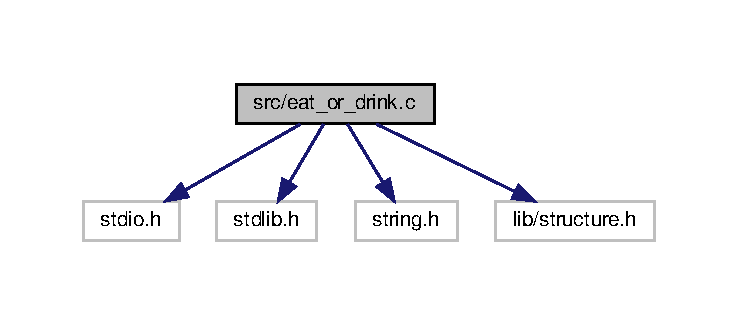
\includegraphics[width=350pt]{eat__or__drink_8c__incl}
\end{center}
\end{figure}
\subsection*{Fonctions}
\begin{DoxyCompactItemize}
\item 
void \hyperlink{eat__or__drink_8c_a400e5d6c52a35b165053c2475905d656}{gain\+\_\+energie} (perso\+\_\+t $\ast$player, int val\+\_\+e)
\begin{DoxyCompactList}\small\item\em Calcule et met à jour les points d\textquotesingle{}énergie du joueur selon la valeur énergétique de l\textquotesingle{}item mangé / bu. \end{DoxyCompactList}\item 
void \hyperlink{eat__or__drink_8c_ab3d3633d751f914bb3b4609a9950c513}{eat\+\_\+or\+\_\+drink} (perso\+\_\+t $\ast$player, item\+\_\+t item)
\begin{DoxyCompactList}\small\item\em Permet au joueur de boire ou manger un item de type {\itshape food} et récupérer des points d\textquotesingle{}énergie ou action (si cela est possible). \end{DoxyCompactList}\end{DoxyCompactItemize}


\subsection{Description détaillée}
Fonctionnalité \+: manger ou boire un item de son inventaire. 

\begin{DoxyAuthor}{Auteur}
Mathilde Mottay, Anaïs Mottier, Clément Mainguy, Moustapha Tsamarayev 
\end{DoxyAuthor}
\begin{DoxyVersion}{Version}
1.\+0 
\end{DoxyVersion}
\begin{DoxyDate}{Date}
2020 
\end{DoxyDate}


\subsection{Documentation des fonctions}
\mbox{\Hypertarget{eat__or__drink_8c_ab3d3633d751f914bb3b4609a9950c513}\label{eat__or__drink_8c_ab3d3633d751f914bb3b4609a9950c513}} 
\index{eat\+\_\+or\+\_\+drink.\+c@{eat\+\_\+or\+\_\+drink.\+c}!eat\+\_\+or\+\_\+drink@{eat\+\_\+or\+\_\+drink}}
\index{eat\+\_\+or\+\_\+drink@{eat\+\_\+or\+\_\+drink}!eat\+\_\+or\+\_\+drink.\+c@{eat\+\_\+or\+\_\+drink.\+c}}
\subsubsection{\texorpdfstring{eat\+\_\+or\+\_\+drink()}{eat\_or\_drink()}}
{\footnotesize\ttfamily void eat\+\_\+or\+\_\+drink (\begin{DoxyParamCaption}\item[{perso\+\_\+t $\ast$}]{player,  }\item[{item\+\_\+t}]{item }\end{DoxyParamCaption})}



Permet au joueur de boire ou manger un item de type {\itshape food} et récupérer des points d\textquotesingle{}énergie ou action (si cela est possible). 

Retire l\textquotesingle{}item de l\textquotesingle{}inventaire 
\begin{DoxyParams}{Paramètres}
{\em perso\+\_\+t} & $\ast$ player \\
\hline
{\em item\+\_\+t} & item \\
\hline
\end{DoxyParams}
\begin{DoxyReturn}{Renvoie}
Rien 
\end{DoxyReturn}
\mbox{\Hypertarget{eat__or__drink_8c_a400e5d6c52a35b165053c2475905d656}\label{eat__or__drink_8c_a400e5d6c52a35b165053c2475905d656}} 
\index{eat\+\_\+or\+\_\+drink.\+c@{eat\+\_\+or\+\_\+drink.\+c}!gain\+\_\+energie@{gain\+\_\+energie}}
\index{gain\+\_\+energie@{gain\+\_\+energie}!eat\+\_\+or\+\_\+drink.\+c@{eat\+\_\+or\+\_\+drink.\+c}}
\subsubsection{\texorpdfstring{gain\+\_\+energie()}{gain\_energie()}}
{\footnotesize\ttfamily void gain\+\_\+energie (\begin{DoxyParamCaption}\item[{perso\+\_\+t $\ast$}]{player,  }\item[{int}]{val\+\_\+e }\end{DoxyParamCaption})}



Calcule et met à jour les points d\textquotesingle{}énergie du joueur selon la valeur énergétique de l\textquotesingle{}item mangé / bu. 


\begin{DoxyParams}{Paramètres}
{\em perso\+\_\+t} & $\ast$ player \\
\hline
{\em int} & val\+\_\+e \\
\hline
\end{DoxyParams}
\begin{DoxyReturn}{Renvoie}
Rien 
\end{DoxyReturn}

\hypertarget{equipment_8c}{}\section{Référence du fichier src/equipment.c}
\label{equipment_8c}\index{src/equipment.\+c@{src/equipment.\+c}}


Gestion de l\textquotesingle{}équipement du joueur.  


{\ttfamily \#include $<$stdio.\+h$>$}\newline
{\ttfamily \#include $<$stdlib.\+h$>$}\newline
{\ttfamily \#include $<$string.\+h$>$}\newline
{\ttfamily \#include $<$unistd.\+h$>$}\newline
{\ttfamily \#include \char`\"{}lib/commun.\+h\char`\"{}}\newline
Graphe des dépendances par inclusion de equipment.\+c\+:
\nopagebreak
\begin{figure}[H]
\begin{center}
\leavevmode
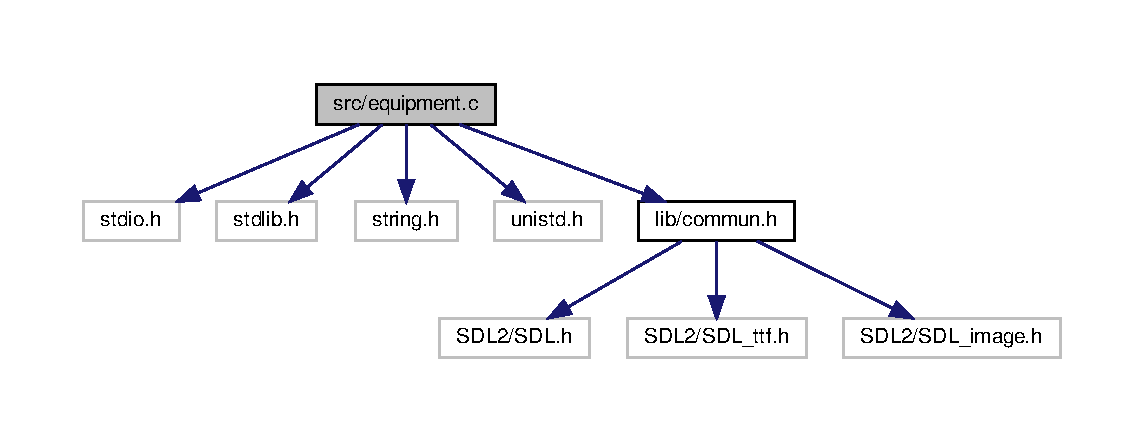
\includegraphics[width=350pt]{equipment_8c__incl}
\end{center}
\end{figure}
\subsection*{Fonctions}
\begin{DoxyCompactItemize}
\item 
void \hyperlink{equipment_8c_ac912edb0758df17f229cb8d8fbd66924}{display\+\_\+equipment\+\_\+player} (\hyperlink{structperso__t}{perso\+\_\+t} player)
\begin{DoxyCompactList}\small\item\em Affiche l\textquotesingle{}équipement du joueur. \end{DoxyCompactList}\item 
int \hyperlink{equipment_8c_aae5f9602614f22807a8f2719fb015bdd}{is\+\_\+equipped} (\hyperlink{structperso__t}{perso\+\_\+t} player, \hyperlink{structitem__t}{item\+\_\+t} item)
\begin{DoxyCompactList}\small\item\em Indique si le joueur est équipé de l\textquotesingle{}item passé en paramètre. \end{DoxyCompactList}\item 
void \hyperlink{equipment_8c_a57d50802c8c7e012de81cff1ddd2082b}{swap\+\_\+equipment\+\_\+player} (\hyperlink{structperso__t}{perso\+\_\+t} $\ast$player, \hyperlink{structitem__t}{item\+\_\+t} item)
\begin{DoxyCompactList}\small\item\em Echange l\textquotesingle{}item passé en paramètre avec un item choisi par le joueur figurant dans son équipement. \end{DoxyCompactList}\item 
void \hyperlink{equipment_8c_a4d4996c52c0585012b5efe58652892ee}{equip\+\_\+player} (\hyperlink{structperso__t}{perso\+\_\+t} $\ast$player)
\begin{DoxyCompactList}\small\item\em Equipe le joueur, au bon endroit, avec un item de son inventaire qu\textquotesingle{}il choisit. \end{DoxyCompactList}\item 
int \hyperlink{equipment_8c_a588235e6d46f215c009c995d07f31ec2}{nb\+\_\+equipement} (\hyperlink{structperso__t}{perso\+\_\+t} player)
\begin{DoxyCompactList}\small\item\em Compte le nombre d\textquotesingle{}item(s) équipé(s) sur le joueur. \end{DoxyCompactList}\item 
int \hyperlink{equipment_8c_aee9562729defb895c78533429b4cb649}{nb\+\_\+items\+\_\+equipables\+\_\+non\+\_\+equipe} (\hyperlink{structperso__t}{perso\+\_\+t} player)
\begin{DoxyCompactList}\small\item\em Compte le nombre d\textquotesingle{}item(s) équipable(s) (armes et armures) mais non équipé(s) que le joueur a dans son inventaire. \end{DoxyCompactList}\item 
void \hyperlink{equipment_8c_a8b6ea8682d1d39157f54a7a84f7020ce}{remove\+\_\+equipment\+\_\+player} (\hyperlink{structperso__t}{perso\+\_\+t} $\ast$player)
\begin{DoxyCompactList}\small\item\em Retire un item choisi par le joueur de son équipement. \end{DoxyCompactList}\item 
void \hyperlink{equipment_8c_afe6c66728ce22be9ff976516f8b77c68}{manage\+\_\+equipment} (\hyperlink{structperso__t}{perso\+\_\+t} $\ast$player)
\begin{DoxyCompactList}\small\item\em Fonction centrale du fichier \hyperlink{equipment_8c}{equipment.\+c} permettant au joueur de gérer son équipement. \end{DoxyCompactList}\end{DoxyCompactItemize}


\subsection{Description détaillée}
Gestion de l\textquotesingle{}équipement du joueur. 

\begin{DoxyAuthor}{Auteur}
Mathilde Mottay, Anaïs Mottier, Clément Mainguy, Moustapha Tsamarayev 
\end{DoxyAuthor}
\begin{DoxyVersion}{Version}
1.\+0 
\end{DoxyVersion}
\begin{DoxyDate}{Date}
2020 
\end{DoxyDate}


\subsection{Documentation des fonctions}
\mbox{\Hypertarget{equipment_8c_ac912edb0758df17f229cb8d8fbd66924}\label{equipment_8c_ac912edb0758df17f229cb8d8fbd66924}} 
\index{equipment.\+c@{equipment.\+c}!display\+\_\+equipment\+\_\+player@{display\+\_\+equipment\+\_\+player}}
\index{display\+\_\+equipment\+\_\+player@{display\+\_\+equipment\+\_\+player}!equipment.\+c@{equipment.\+c}}
\subsubsection{\texorpdfstring{display\+\_\+equipment\+\_\+player()}{display\_equipment\_player()}}
{\footnotesize\ttfamily void display\+\_\+equipment\+\_\+player (\begin{DoxyParamCaption}\item[{\hyperlink{structperso__t}{perso\+\_\+t}}]{player }\end{DoxyParamCaption})}



Affiche l\textquotesingle{}équipement du joueur. 

Si la tête, la main gauche, la main droite ou le corps du joueur sont équipés, indique avec quels items en précisant leurs positions dans l\textquotesingle{}inventaire. 
\begin{DoxyParams}{Paramètres}
{\em player} & Joueur \\
\hline
\end{DoxyParams}
\begin{DoxyReturn}{Renvoie}
Rien 
\end{DoxyReturn}
\mbox{\Hypertarget{equipment_8c_a4d4996c52c0585012b5efe58652892ee}\label{equipment_8c_a4d4996c52c0585012b5efe58652892ee}} 
\index{equipment.\+c@{equipment.\+c}!equip\+\_\+player@{equip\+\_\+player}}
\index{equip\+\_\+player@{equip\+\_\+player}!equipment.\+c@{equipment.\+c}}
\subsubsection{\texorpdfstring{equip\+\_\+player()}{equip\_player()}}
{\footnotesize\ttfamily void equip\+\_\+player (\begin{DoxyParamCaption}\item[{\hyperlink{structperso__t}{perso\+\_\+t} $\ast$}]{player }\end{DoxyParamCaption})}



Equipe le joueur, au bon endroit, avec un item de son inventaire qu\textquotesingle{}il choisit. 

L\textquotesingle{}item doit être équipable. 
\begin{DoxyParams}{Paramètres}
{\em player} & Pointeur sur un objet de type \hyperlink{structperso__t}{perso\+\_\+t} correspond au joueur \\
\hline
\end{DoxyParams}
\begin{DoxyReturn}{Renvoie}
Rien 
\end{DoxyReturn}
\mbox{\Hypertarget{equipment_8c_aae5f9602614f22807a8f2719fb015bdd}\label{equipment_8c_aae5f9602614f22807a8f2719fb015bdd}} 
\index{equipment.\+c@{equipment.\+c}!is\+\_\+equipped@{is\+\_\+equipped}}
\index{is\+\_\+equipped@{is\+\_\+equipped}!equipment.\+c@{equipment.\+c}}
\subsubsection{\texorpdfstring{is\+\_\+equipped()}{is\_equipped()}}
{\footnotesize\ttfamily int is\+\_\+equipped (\begin{DoxyParamCaption}\item[{\hyperlink{structperso__t}{perso\+\_\+t}}]{player,  }\item[{\hyperlink{structitem__t}{item\+\_\+t}}]{item }\end{DoxyParamCaption})}



Indique si le joueur est équipé de l\textquotesingle{}item passé en paramètre. 


\begin{DoxyParams}{Paramètres}
{\em player} & Joueur \\
\hline
{\em item} & Item \\
\hline
\end{DoxyParams}
\begin{DoxyReturn}{Renvoie}
Un {\itshape int} \+: si le joueur n\textquotesingle{}est pas équipé de l\textquotesingle{}item retourne 0 (\hyperlink{commun_8h_a6764330ff4f04cee324e30f775960f02}{N\+O\+T\+\_\+\+E\+Q\+U\+I\+P\+P\+ED}), sinon retourne où l\textquotesingle{}item est équipé sur le joueur (\hyperlink{commun_8h_a2eff09387fb5d20d8af4fa186ae37c4d}{L\+E\+F\+T\+\_\+\+H\+A\+ND} = 1, \hyperlink{commun_8h_a5d1d275cfec76197e014fe4d58f2e569}{R\+I\+G\+H\+T\+\_\+\+H\+A\+ND} = 2, \hyperlink{commun_8h_aa6bdf6a6d9916c343e1e17774d84a156}{B\+O\+DY} = 3, \hyperlink{commun_8h_a110f3b6cdacd45daee818b3e5965f6da}{H\+E\+AD} = 4) 
\end{DoxyReturn}
\mbox{\Hypertarget{equipment_8c_afe6c66728ce22be9ff976516f8b77c68}\label{equipment_8c_afe6c66728ce22be9ff976516f8b77c68}} 
\index{equipment.\+c@{equipment.\+c}!manage\+\_\+equipment@{manage\+\_\+equipment}}
\index{manage\+\_\+equipment@{manage\+\_\+equipment}!equipment.\+c@{equipment.\+c}}
\subsubsection{\texorpdfstring{manage\+\_\+equipment()}{manage\_equipment()}}
{\footnotesize\ttfamily void manage\+\_\+equipment (\begin{DoxyParamCaption}\item[{\hyperlink{structperso__t}{perso\+\_\+t} $\ast$}]{player }\end{DoxyParamCaption})}



Fonction centrale du fichier \hyperlink{equipment_8c}{equipment.\+c} permettant au joueur de gérer son équipement. 

Menu équipement \+: Possibilité pour le joueur de s\textquotesingle{}équiper d\textquotesingle{}un item de son inventaire, de retirer un item de son équipement. 
\begin{DoxyParams}{Paramètres}
{\em player} & Pointeur sur un objet de type \hyperlink{structperso__t}{perso\+\_\+t} correspondant au joueur \\
\hline
\end{DoxyParams}
\begin{DoxyReturn}{Renvoie}
Rien 
\end{DoxyReturn}
\mbox{\Hypertarget{equipment_8c_a588235e6d46f215c009c995d07f31ec2}\label{equipment_8c_a588235e6d46f215c009c995d07f31ec2}} 
\index{equipment.\+c@{equipment.\+c}!nb\+\_\+equipement@{nb\+\_\+equipement}}
\index{nb\+\_\+equipement@{nb\+\_\+equipement}!equipment.\+c@{equipment.\+c}}
\subsubsection{\texorpdfstring{nb\+\_\+equipement()}{nb\_equipement()}}
{\footnotesize\ttfamily int nb\+\_\+equipement (\begin{DoxyParamCaption}\item[{\hyperlink{structperso__t}{perso\+\_\+t}}]{player }\end{DoxyParamCaption})}



Compte le nombre d\textquotesingle{}item(s) équipé(s) sur le joueur. 


\begin{DoxyParams}{Paramètres}
{\em player} & Joueur \\
\hline
\end{DoxyParams}
\begin{DoxyReturn}{Renvoie}
Un {\itshape int} correspondant au nombre d\textquotesingle{}équipement(s) (items) actuellement sur le joueur 
\end{DoxyReturn}
\mbox{\Hypertarget{equipment_8c_aee9562729defb895c78533429b4cb649}\label{equipment_8c_aee9562729defb895c78533429b4cb649}} 
\index{equipment.\+c@{equipment.\+c}!nb\+\_\+items\+\_\+equipables\+\_\+non\+\_\+equipe@{nb\+\_\+items\+\_\+equipables\+\_\+non\+\_\+equipe}}
\index{nb\+\_\+items\+\_\+equipables\+\_\+non\+\_\+equipe@{nb\+\_\+items\+\_\+equipables\+\_\+non\+\_\+equipe}!equipment.\+c@{equipment.\+c}}
\subsubsection{\texorpdfstring{nb\+\_\+items\+\_\+equipables\+\_\+non\+\_\+equipe()}{nb\_items\_equipables\_non\_equipe()}}
{\footnotesize\ttfamily int nb\+\_\+items\+\_\+equipables\+\_\+non\+\_\+equipe (\begin{DoxyParamCaption}\item[{\hyperlink{structperso__t}{perso\+\_\+t}}]{player }\end{DoxyParamCaption})}



Compte le nombre d\textquotesingle{}item(s) équipable(s) (armes et armures) mais non équipé(s) que le joueur a dans son inventaire. 


\begin{DoxyParams}{Paramètres}
{\em player} & Joueur \\
\hline
\end{DoxyParams}
\begin{DoxyReturn}{Renvoie}
Un {\itshape int} correspondant au nombre d\textquotesingle{}équipement(s) équipable(s) mais non équipé(s) que le joueur a dans son inventaire 
\end{DoxyReturn}
\mbox{\Hypertarget{equipment_8c_a8b6ea8682d1d39157f54a7a84f7020ce}\label{equipment_8c_a8b6ea8682d1d39157f54a7a84f7020ce}} 
\index{equipment.\+c@{equipment.\+c}!remove\+\_\+equipment\+\_\+player@{remove\+\_\+equipment\+\_\+player}}
\index{remove\+\_\+equipment\+\_\+player@{remove\+\_\+equipment\+\_\+player}!equipment.\+c@{equipment.\+c}}
\subsubsection{\texorpdfstring{remove\+\_\+equipment\+\_\+player()}{remove\_equipment\_player()}}
{\footnotesize\ttfamily void remove\+\_\+equipment\+\_\+player (\begin{DoxyParamCaption}\item[{\hyperlink{structperso__t}{perso\+\_\+t} $\ast$}]{player }\end{DoxyParamCaption})}



Retire un item choisi par le joueur de son équipement. 


\begin{DoxyParams}{Paramètres}
{\em player} & Pointeur sur un objet de type \hyperlink{structperso__t}{perso\+\_\+t} correspondant au joueur \\
\hline
\end{DoxyParams}
\begin{DoxyReturn}{Renvoie}
Rien 
\end{DoxyReturn}
\mbox{\Hypertarget{equipment_8c_a57d50802c8c7e012de81cff1ddd2082b}\label{equipment_8c_a57d50802c8c7e012de81cff1ddd2082b}} 
\index{equipment.\+c@{equipment.\+c}!swap\+\_\+equipment\+\_\+player@{swap\+\_\+equipment\+\_\+player}}
\index{swap\+\_\+equipment\+\_\+player@{swap\+\_\+equipment\+\_\+player}!equipment.\+c@{equipment.\+c}}
\subsubsection{\texorpdfstring{swap\+\_\+equipment\+\_\+player()}{swap\_equipment\_player()}}
{\footnotesize\ttfamily void swap\+\_\+equipment\+\_\+player (\begin{DoxyParamCaption}\item[{\hyperlink{structperso__t}{perso\+\_\+t} $\ast$}]{player,  }\item[{\hyperlink{structitem__t}{item\+\_\+t}}]{item }\end{DoxyParamCaption})}



Echange l\textquotesingle{}item passé en paramètre avec un item choisi par le joueur figurant dans son équipement. 

Cette fonction est appelée lorsque le joueur souhaite s\textquotesingle{}équiper d\textquotesingle{}un item sur une zone de son corps déjà équipée. 
\begin{DoxyParams}{Paramètres}
{\em player} & Pointeur sur un objet de type \hyperlink{structperso__t}{perso\+\_\+t} correspond au joueur \\
\hline
{\em item} & Item \\
\hline
\end{DoxyParams}
\begin{DoxyReturn}{Renvoie}
Rien 
\end{DoxyReturn}

\hypertarget{exit__help_8c}{}\section{Référence du fichier src/exit\+\_\+help.c}
\label{exit__help_8c}\index{src/exit\+\_\+help.\+c@{src/exit\+\_\+help.\+c}}


Sortie + Aide.  


{\ttfamily \#include $<$stdio.\+h$>$}\newline
{\ttfamily \#include $<$stdlib.\+h$>$}\newline
{\ttfamily \#include $<$string.\+h$>$}\newline
{\ttfamily \#include $<$time.\+h$>$}\newline
{\ttfamily \#include $<$unistd.\+h$>$}\newline
{\ttfamily \#include \char`\"{}lib/structure.\+h\char`\"{}}\newline
Graphe des dépendances par inclusion de exit\+\_\+help.\+c\+:\nopagebreak
\begin{figure}[H]
\begin{center}
\leavevmode
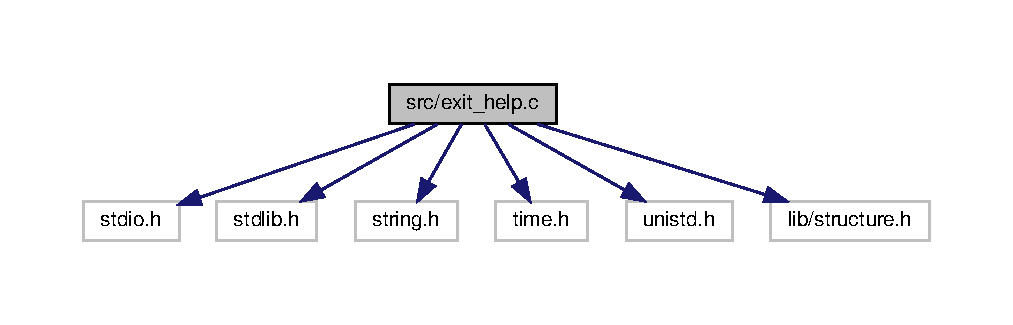
\includegraphics[width=350pt]{exit__help_8c__incl}
\end{center}
\end{figure}
\subsection*{Fonctions}
\begin{DoxyCompactItemize}
\item 
int \hyperlink{exit__help_8c_afd7728c9e6ae89e5932e641b54556aba}{exit\+\_\+game} ()
\begin{DoxyCompactList}\small\item\em Propose au joueur de quitter ou non la carte lorsqu\textquotesingle{}il vient de trouver la sortie. \end{DoxyCompactList}\item 
void \hyperlink{exit__help_8c_aa837a09de6dddbefdb7b6f86b8f1f833}{help} (perso\+\_\+t $\ast$player)
\begin{DoxyCompactList}\small\item\em Donne des conseils au joueur suivant ses difficultés. \end{DoxyCompactList}\end{DoxyCompactItemize}


\subsection{Description détaillée}
Sortie + Aide. 

\begin{DoxyAuthor}{Auteur}
Mathilde Mottay, Anaïs Mottier, Clément Mainguy, Moustapha Tsamarayev 
\end{DoxyAuthor}
\begin{DoxyVersion}{Version}

\end{DoxyVersion}
\begin{DoxyDate}{Date}
2020 
\end{DoxyDate}


\subsection{Documentation des fonctions}
\mbox{\Hypertarget{exit__help_8c_afd7728c9e6ae89e5932e641b54556aba}\label{exit__help_8c_afd7728c9e6ae89e5932e641b54556aba}} 
\index{exit\+\_\+help.\+c@{exit\+\_\+help.\+c}!exit\+\_\+game@{exit\+\_\+game}}
\index{exit\+\_\+game@{exit\+\_\+game}!exit\+\_\+help.\+c@{exit\+\_\+help.\+c}}
\subsubsection{\texorpdfstring{exit\+\_\+game()}{exit\_game()}}
{\footnotesize\ttfamily int exit\+\_\+game (\begin{DoxyParamCaption}{ }\end{DoxyParamCaption})}



Propose au joueur de quitter ou non la carte lorsqu\textquotesingle{}il vient de trouver la sortie. 

\begin{DoxyReturn}{Renvoie}
Un {\itshape int} \+: 1 si le joueur décide de quitter la carte. 0 s\textquotesingle{}il décide de continuer l\textquotesingle{}aventure. 
\end{DoxyReturn}
\mbox{\Hypertarget{exit__help_8c_aa837a09de6dddbefdb7b6f86b8f1f833}\label{exit__help_8c_aa837a09de6dddbefdb7b6f86b8f1f833}} 
\index{exit\+\_\+help.\+c@{exit\+\_\+help.\+c}!help@{help}}
\index{help@{help}!exit\+\_\+help.\+c@{exit\+\_\+help.\+c}}
\subsubsection{\texorpdfstring{help()}{help()}}
{\footnotesize\ttfamily void help (\begin{DoxyParamCaption}\item[{perso\+\_\+t $\ast$}]{player }\end{DoxyParamCaption})}



Donne des conseils au joueur suivant ses difficultés. 


\begin{DoxyParams}{Paramètres}
{\em perso\+\_\+t} & $\ast$ player \\
\hline
\end{DoxyParams}
\begin{DoxyReturn}{Renvoie}
Rien 
\end{DoxyReturn}

\hypertarget{fish_8c}{}\section{Référence du fichier src/fish.c}
\label{fish_8c}\index{src/fish.\+c@{src/fish.\+c}}


Fonctionnalité \+: pêcher.  


{\ttfamily \#include $<$stdio.\+h$>$}\newline
{\ttfamily \#include $<$stdlib.\+h$>$}\newline
{\ttfamily \#include $<$string.\+h$>$}\newline
{\ttfamily \#include $<$time.\+h$>$}\newline
{\ttfamily \#include $<$unistd.\+h$>$}\newline
{\ttfamily \#include \char`\"{}lib/structure.\+h\char`\"{}}\newline
Graphe des dépendances par inclusion de fish.\+c\+:\nopagebreak
\begin{figure}[H]
\begin{center}
\leavevmode
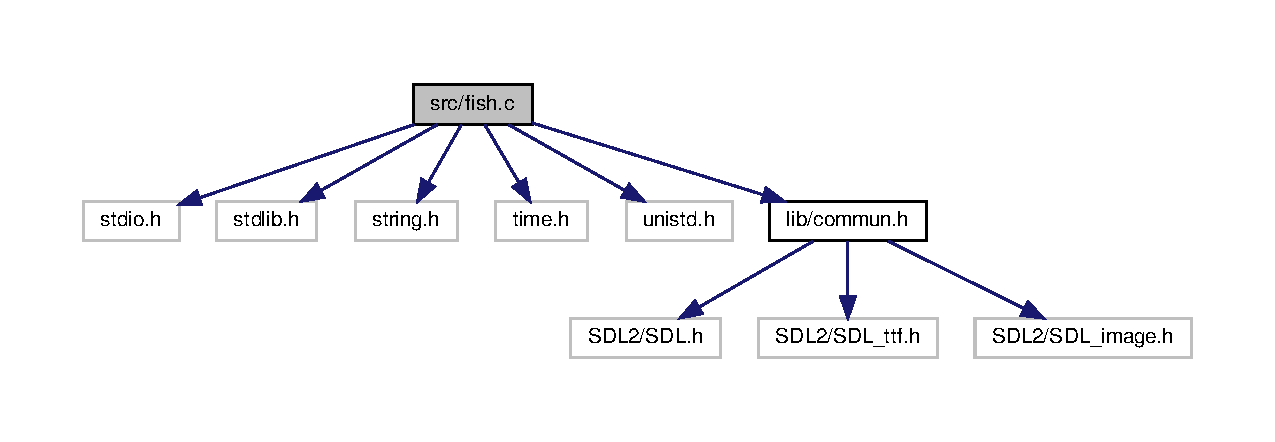
\includegraphics[width=350pt]{fish_8c__incl}
\end{center}
\end{figure}
\subsection*{Fonctions}
\begin{DoxyCompactItemize}
\item 
void \hyperlink{fish_8c_aec4be0e1e14efa931211be073ea33cab}{fish} (perso\+\_\+t $\ast$player, cell\+\_\+t map\mbox{[}D\mbox{]}\mbox{[}D\mbox{]})
\begin{DoxyCompactList}\small\item\em Permet au joueur de pêcher s\textquotesingle{}il se situe sur un hexagone de type {\itshape lac} ou {\itshape mer} et s\textquotesingle{}il a une canne à pêche dans son inventaire. \end{DoxyCompactList}\end{DoxyCompactItemize}


\subsection{Description détaillée}
Fonctionnalité \+: pêcher. 

\begin{DoxyAuthor}{Auteur}
Mathilde Mottay, Anaïs Mottier, Clément Mainguy, Moustapha Tsamarayev 
\end{DoxyAuthor}
\begin{DoxyVersion}{Version}
1.\+0 
\end{DoxyVersion}
\begin{DoxyDate}{Date}
2020 
\end{DoxyDate}


\subsection{Documentation des fonctions}
\mbox{\Hypertarget{fish_8c_aec4be0e1e14efa931211be073ea33cab}\label{fish_8c_aec4be0e1e14efa931211be073ea33cab}} 
\index{fish.\+c@{fish.\+c}!fish@{fish}}
\index{fish@{fish}!fish.\+c@{fish.\+c}}
\subsubsection{\texorpdfstring{fish()}{fish()}}
{\footnotesize\ttfamily void fish (\begin{DoxyParamCaption}\item[{perso\+\_\+t $\ast$}]{player,  }\item[{cell\+\_\+t}]{map\mbox{[}\+D\mbox{]}\mbox{[}\+D\mbox{]} }\end{DoxyParamCaption})}



Permet au joueur de pêcher s\textquotesingle{}il se situe sur un hexagone de type {\itshape lac} ou {\itshape mer} et s\textquotesingle{}il a une canne à pêche dans son inventaire. 


\begin{DoxyParams}{Paramètres}
{\em perso\+\_\+t} & $\ast$ player \\
\hline
{\em cell\+\_\+t} & map\mbox{[}D\mbox{]}\mbox{[}D\mbox{]} \\
\hline
\end{DoxyParams}
\begin{DoxyReturn}{Renvoie}
Rien 
\end{DoxyReturn}

\hypertarget{inventory_8c}{}\section{Référence du fichier src/inventory.c}
\label{inventory_8c}\index{src/inventory.\+c@{src/inventory.\+c}}


Gestion de l\textquotesingle{}inventaire du joueur.  


{\ttfamily \#include $<$stdio.\+h$>$}\newline
{\ttfamily \#include $<$stdlib.\+h$>$}\newline
{\ttfamily \#include $<$string.\+h$>$}\newline
{\ttfamily \#include $<$time.\+h$>$}\newline
{\ttfamily \#include $<$unistd.\+h$>$}\newline
{\ttfamily \#include \char`\"{}lib/commun.\+h\char`\"{}}\newline
Graphe des dépendances par inclusion de inventory.\+c\+:\nopagebreak
\begin{figure}[H]
\begin{center}
\leavevmode
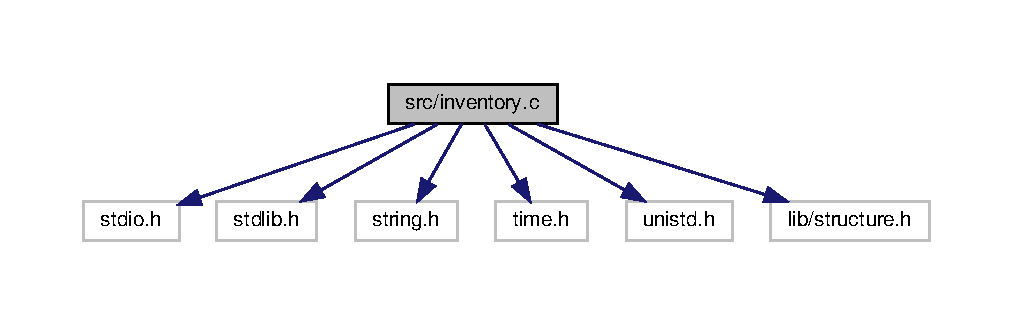
\includegraphics[width=350pt]{inventory_8c__incl}
\end{center}
\end{figure}
\subsection*{Fonctions}
\begin{DoxyCompactItemize}
\item 
void \hyperlink{inventory_8c_a400e5d6c52a35b165053c2475905d656}{gain\+\_\+energie} (\hyperlink{structperso__t}{perso\+\_\+t} $\ast$player, int val\+\_\+e)
\begin{DoxyCompactList}\small\item\em Calcule et met à jour les points d\textquotesingle{}énergie du joueur selon la valeur énergétique de l\textquotesingle{}item mangé / bu. \end{DoxyCompactList}\item 
void \hyperlink{inventory_8c_ab3d3633d751f914bb3b4609a9950c513}{eat\+\_\+or\+\_\+drink} (\hyperlink{structperso__t}{perso\+\_\+t} $\ast$player, \hyperlink{structitem__t}{item\+\_\+t} item)
\begin{DoxyCompactList}\small\item\em Permet au joueur de boire ou manger un item de type {\itshape food} et récupérer des points d\textquotesingle{}énergie ou action (si cela est possible). \end{DoxyCompactList}\item 
void \hyperlink{inventory_8c_a08b9c4c266cfcf2e07d74de53285d88f}{check\+\_\+the\+\_\+map} (\hyperlink{structperso__t}{perso\+\_\+t} player, \hyperlink{structcell__t}{cell\+\_\+t} map\mbox{[}\hyperlink{commun_8h_af316c33cc298530f245e8b55330e86b5}{D}\mbox{]}\mbox{[}\hyperlink{commun_8h_af316c33cc298530f245e8b55330e86b5}{D}\mbox{]})
\begin{DoxyCompactList}\small\item\em Affiche la carte, si le joueur en possède une dans son inventaire. \end{DoxyCompactList}\item 
int \hyperlink{inventory_8c_a422fba7d76e9ed4b5783cf5d9177aad8}{item\+\_\+in\+\_\+inventory} (\hyperlink{structperso__t}{perso\+\_\+t} player, char $\ast$nom\+\_\+item)
\begin{DoxyCompactList}\small\item\em Recherche si l\textquotesingle{}item dont le nom est passé en paramètre est présent ou non dans l\textquotesingle{}inventaire. \end{DoxyCompactList}\item 
int \hyperlink{inventory_8c_a74d9dc2f174857b3bf7ec5453faae17e}{food\+\_\+in\+\_\+inventory} (\hyperlink{structperso__t}{perso\+\_\+t} player)
\begin{DoxyCompactList}\small\item\em Calcule le nombre d\textquotesingle{}items {\itshape food} dans l\textquotesingle{}inventaire du joueur. \end{DoxyCompactList}\item 
int \hyperlink{inventory_8c_ae86124ec1e7b0d9c46acbd4327e9885d}{too\+\_\+much\+\_\+of\+\_\+the\+\_\+same\+\_\+item} (\hyperlink{structperso__t}{perso\+\_\+t} player, \hyperlink{structitem__t}{item\+\_\+t} item)
\begin{DoxyCompactList}\small\item\em Indique si l\textquotesingle{}item passé en paramètre apparaît 2 fois ou plus dans l\textquotesingle{}inventaire du joueur. \end{DoxyCompactList}\item 
void \hyperlink{inventory_8c_a354d78a490ef30d40f4a726524090b21}{display\+\_\+inventory} (\hyperlink{structperso__t}{perso\+\_\+t} player)
\begin{DoxyCompactList}\small\item\em Affiche l\textquotesingle{}inventaire du joueur. \end{DoxyCompactList}\item 
void \hyperlink{inventory_8c_a9bc6d36c93298c7aead4ea6e7e6e3e26}{delete\+\_\+item\+\_\+in\+\_\+inventory} (\hyperlink{structperso__t}{perso\+\_\+t} $\ast$player, \hyperlink{structitem__t}{item\+\_\+t} item)
\begin{DoxyCompactList}\small\item\em Retire l\textquotesingle{}item passé en paramètre de l\textquotesingle{}inventaire (et de l\textquotesingle{}équipement si besoin) du joueur. \end{DoxyCompactList}\item 
int \hyperlink{inventory_8c_a1668516cd0e1d31746805efdbd4a5f34}{add\+\_\+item\+\_\+to\+\_\+inventory} (\hyperlink{structperso__t}{perso\+\_\+t} $\ast$player, \hyperlink{structitem__t}{item\+\_\+t} item)
\begin{DoxyCompactList}\small\item\em Ajoute un item à l\textquotesingle{}inventaire du joueur. \end{DoxyCompactList}\item 
void \hyperlink{inventory_8c_a35b519c6835c9aa90ff5fd35b0e68f66}{manage\+\_\+inventory} (\hyperlink{structperso__t}{perso\+\_\+t} $\ast$player)
\begin{DoxyCompactList}\small\item\em Fonction centrale du fichier \hyperlink{inventory_8c}{inventory.\+c} permettant au joueur de gérer son inventaire. \end{DoxyCompactList}\end{DoxyCompactItemize}


\subsection{Description détaillée}
Gestion de l\textquotesingle{}inventaire du joueur. 

\begin{DoxyAuthor}{Auteur}
Mathilde Mottay, Anaïs Mottier, Clément Mainguy, Moustapha Tsamarayev 
\end{DoxyAuthor}
\begin{DoxyVersion}{Version}
1.\+0 
\end{DoxyVersion}
\begin{DoxyDate}{Date}
2020 
\end{DoxyDate}


\subsection{Documentation des fonctions}
\mbox{\Hypertarget{inventory_8c_a1668516cd0e1d31746805efdbd4a5f34}\label{inventory_8c_a1668516cd0e1d31746805efdbd4a5f34}} 
\index{inventory.\+c@{inventory.\+c}!add\+\_\+item\+\_\+to\+\_\+inventory@{add\+\_\+item\+\_\+to\+\_\+inventory}}
\index{add\+\_\+item\+\_\+to\+\_\+inventory@{add\+\_\+item\+\_\+to\+\_\+inventory}!inventory.\+c@{inventory.\+c}}
\subsubsection{\texorpdfstring{add\+\_\+item\+\_\+to\+\_\+inventory()}{add\_item\_to\_inventory()}}
{\footnotesize\ttfamily int add\+\_\+item\+\_\+to\+\_\+inventory (\begin{DoxyParamCaption}\item[{\hyperlink{structperso__t}{perso\+\_\+t} $\ast$}]{player,  }\item[{\hyperlink{structitem__t}{item\+\_\+t}}]{item }\end{DoxyParamCaption})}



Ajoute un item à l\textquotesingle{}inventaire du joueur. 

Si son inventaire est plein, propose un échange. 
\begin{DoxyParams}{Paramètres}
{\em player} & Pointeur sur un objet de type \hyperlink{structperso__t}{perso\+\_\+t} correspondant au joueur \\
\hline
{\em item} & Item à ajouter à l\textquotesingle{}inventaire \\
\hline
\end{DoxyParams}
\begin{DoxyReturn}{Renvoie}
Un {\itshape int} \+: 1 si ajout effectué. 0 sinon. 
\end{DoxyReturn}
\mbox{\Hypertarget{inventory_8c_a08b9c4c266cfcf2e07d74de53285d88f}\label{inventory_8c_a08b9c4c266cfcf2e07d74de53285d88f}} 
\index{inventory.\+c@{inventory.\+c}!check\+\_\+the\+\_\+map@{check\+\_\+the\+\_\+map}}
\index{check\+\_\+the\+\_\+map@{check\+\_\+the\+\_\+map}!inventory.\+c@{inventory.\+c}}
\subsubsection{\texorpdfstring{check\+\_\+the\+\_\+map()}{check\_the\_map()}}
{\footnotesize\ttfamily void check\+\_\+the\+\_\+map (\begin{DoxyParamCaption}\item[{\hyperlink{structperso__t}{perso\+\_\+t}}]{player,  }\item[{\hyperlink{structcell__t}{cell\+\_\+t}}]{map\mbox{[}\+D\mbox{]}\mbox{[}\+D\mbox{]} }\end{DoxyParamCaption})}



Affiche la carte, si le joueur en possède une dans son inventaire. 


\begin{DoxyParams}{Paramètres}
{\em player} & Joueur \\
\hline
{\em map\mbox{[}\+D\mbox{]}\mbox{[}\+D\mbox{]}} & Matrice de la carte \\
\hline
\end{DoxyParams}
\begin{DoxyReturn}{Renvoie}
Rien 
\end{DoxyReturn}
\mbox{\Hypertarget{inventory_8c_a9bc6d36c93298c7aead4ea6e7e6e3e26}\label{inventory_8c_a9bc6d36c93298c7aead4ea6e7e6e3e26}} 
\index{inventory.\+c@{inventory.\+c}!delete\+\_\+item\+\_\+in\+\_\+inventory@{delete\+\_\+item\+\_\+in\+\_\+inventory}}
\index{delete\+\_\+item\+\_\+in\+\_\+inventory@{delete\+\_\+item\+\_\+in\+\_\+inventory}!inventory.\+c@{inventory.\+c}}
\subsubsection{\texorpdfstring{delete\+\_\+item\+\_\+in\+\_\+inventory()}{delete\_item\_in\_inventory()}}
{\footnotesize\ttfamily void delete\+\_\+item\+\_\+in\+\_\+inventory (\begin{DoxyParamCaption}\item[{\hyperlink{structperso__t}{perso\+\_\+t} $\ast$}]{player,  }\item[{\hyperlink{structitem__t}{item\+\_\+t}}]{item }\end{DoxyParamCaption})}



Retire l\textquotesingle{}item passé en paramètre de l\textquotesingle{}inventaire (et de l\textquotesingle{}équipement si besoin) du joueur. 


\begin{DoxyParams}{Paramètres}
{\em player} & Pointeur sur un objet de type \hyperlink{structperso__t}{perso\+\_\+t} correspondant au joueur \\
\hline
{\em item} & Item à retirer de l\textquotesingle{}inventaire \\
\hline
\end{DoxyParams}
\begin{DoxyReturn}{Renvoie}
Rien 
\end{DoxyReturn}
\mbox{\Hypertarget{inventory_8c_a354d78a490ef30d40f4a726524090b21}\label{inventory_8c_a354d78a490ef30d40f4a726524090b21}} 
\index{inventory.\+c@{inventory.\+c}!display\+\_\+inventory@{display\+\_\+inventory}}
\index{display\+\_\+inventory@{display\+\_\+inventory}!inventory.\+c@{inventory.\+c}}
\subsubsection{\texorpdfstring{display\+\_\+inventory()}{display\_inventory()}}
{\footnotesize\ttfamily void display\+\_\+inventory (\begin{DoxyParamCaption}\item[{\hyperlink{structperso__t}{perso\+\_\+t}}]{player }\end{DoxyParamCaption})}



Affiche l\textquotesingle{}inventaire du joueur. 

Affichage des items de l\textquotesingle{}inventaire avec leurs positions, par catégorie (armes, armures, divers, nourriture). Indique si item équipé pour les armes et armures. 
\begin{DoxyParams}{Paramètres}
{\em player} & Joueur \\
\hline
\end{DoxyParams}
\begin{DoxyReturn}{Renvoie}
Rien 
\end{DoxyReturn}
\mbox{\Hypertarget{inventory_8c_ab3d3633d751f914bb3b4609a9950c513}\label{inventory_8c_ab3d3633d751f914bb3b4609a9950c513}} 
\index{inventory.\+c@{inventory.\+c}!eat\+\_\+or\+\_\+drink@{eat\+\_\+or\+\_\+drink}}
\index{eat\+\_\+or\+\_\+drink@{eat\+\_\+or\+\_\+drink}!inventory.\+c@{inventory.\+c}}
\subsubsection{\texorpdfstring{eat\+\_\+or\+\_\+drink()}{eat\_or\_drink()}}
{\footnotesize\ttfamily void eat\+\_\+or\+\_\+drink (\begin{DoxyParamCaption}\item[{\hyperlink{structperso__t}{perso\+\_\+t} $\ast$}]{player,  }\item[{\hyperlink{structitem__t}{item\+\_\+t}}]{item }\end{DoxyParamCaption})}



Permet au joueur de boire ou manger un item de type {\itshape food} et récupérer des points d\textquotesingle{}énergie ou action (si cela est possible). 

Retire l\textquotesingle{}item mangé / bu de l\textquotesingle{}inventaire 
\begin{DoxyParams}{Paramètres}
{\em player} & Pointeur sur un objet de type \hyperlink{structperso__t}{perso\+\_\+t} correspondant au joueur \\
\hline
{\em item} & Item que le joueur désire manger ou boire \\
\hline
\end{DoxyParams}
\begin{DoxyReturn}{Renvoie}
Rien 
\end{DoxyReturn}
\mbox{\Hypertarget{inventory_8c_a74d9dc2f174857b3bf7ec5453faae17e}\label{inventory_8c_a74d9dc2f174857b3bf7ec5453faae17e}} 
\index{inventory.\+c@{inventory.\+c}!food\+\_\+in\+\_\+inventory@{food\+\_\+in\+\_\+inventory}}
\index{food\+\_\+in\+\_\+inventory@{food\+\_\+in\+\_\+inventory}!inventory.\+c@{inventory.\+c}}
\subsubsection{\texorpdfstring{food\+\_\+in\+\_\+inventory()}{food\_in\_inventory()}}
{\footnotesize\ttfamily int food\+\_\+in\+\_\+inventory (\begin{DoxyParamCaption}\item[{\hyperlink{structperso__t}{perso\+\_\+t}}]{player }\end{DoxyParamCaption})}



Calcule le nombre d\textquotesingle{}items {\itshape food} dans l\textquotesingle{}inventaire du joueur. 


\begin{DoxyParams}{Paramètres}
{\em player} & Joueur \\
\hline
\end{DoxyParams}
\begin{DoxyReturn}{Renvoie}
Un {\itshape int} \+: nombre d\textquotesingle{}items {\itshape food} dans l\textquotesingle{}inventaire du joueur 
\end{DoxyReturn}
\mbox{\Hypertarget{inventory_8c_a400e5d6c52a35b165053c2475905d656}\label{inventory_8c_a400e5d6c52a35b165053c2475905d656}} 
\index{inventory.\+c@{inventory.\+c}!gain\+\_\+energie@{gain\+\_\+energie}}
\index{gain\+\_\+energie@{gain\+\_\+energie}!inventory.\+c@{inventory.\+c}}
\subsubsection{\texorpdfstring{gain\+\_\+energie()}{gain\_energie()}}
{\footnotesize\ttfamily void gain\+\_\+energie (\begin{DoxyParamCaption}\item[{\hyperlink{structperso__t}{perso\+\_\+t} $\ast$}]{player,  }\item[{int}]{val\+\_\+e }\end{DoxyParamCaption})}



Calcule et met à jour les points d\textquotesingle{}énergie du joueur selon la valeur énergétique de l\textquotesingle{}item mangé / bu. 


\begin{DoxyParams}{Paramètres}
{\em player} & Pointeur sur un objet de type \hyperlink{structperso__t}{perso\+\_\+t} correspondant au joueur \\
\hline
{\em val\+\_\+e} & Valeur énergétique de l\textquotesingle{}item mangé/bu \\
\hline
\end{DoxyParams}
\begin{DoxyReturn}{Renvoie}
Rien 
\end{DoxyReturn}
\mbox{\Hypertarget{inventory_8c_a422fba7d76e9ed4b5783cf5d9177aad8}\label{inventory_8c_a422fba7d76e9ed4b5783cf5d9177aad8}} 
\index{inventory.\+c@{inventory.\+c}!item\+\_\+in\+\_\+inventory@{item\+\_\+in\+\_\+inventory}}
\index{item\+\_\+in\+\_\+inventory@{item\+\_\+in\+\_\+inventory}!inventory.\+c@{inventory.\+c}}
\subsubsection{\texorpdfstring{item\+\_\+in\+\_\+inventory()}{item\_in\_inventory()}}
{\footnotesize\ttfamily int item\+\_\+in\+\_\+inventory (\begin{DoxyParamCaption}\item[{\hyperlink{structperso__t}{perso\+\_\+t}}]{player,  }\item[{char $\ast$}]{nom\+\_\+item }\end{DoxyParamCaption})}



Recherche si l\textquotesingle{}item dont le nom est passé en paramètre est présent ou non dans l\textquotesingle{}inventaire. 


\begin{DoxyParams}{Paramètres}
{\em player} & Joueur \\
\hline
{\em nom\+\_\+item} & Nom de l\textquotesingle{}item à rechercher dans l\textquotesingle{}inventaire \\
\hline
\end{DoxyParams}
\begin{DoxyReturn}{Renvoie}
Un {\itshape int} \+: position de l\textquotesingle{}item dans l\textquotesingle{}inventaire si présent, -\/1 si absent 
\end{DoxyReturn}
\mbox{\Hypertarget{inventory_8c_a35b519c6835c9aa90ff5fd35b0e68f66}\label{inventory_8c_a35b519c6835c9aa90ff5fd35b0e68f66}} 
\index{inventory.\+c@{inventory.\+c}!manage\+\_\+inventory@{manage\+\_\+inventory}}
\index{manage\+\_\+inventory@{manage\+\_\+inventory}!inventory.\+c@{inventory.\+c}}
\subsubsection{\texorpdfstring{manage\+\_\+inventory()}{manage\_inventory()}}
{\footnotesize\ttfamily void manage\+\_\+inventory (\begin{DoxyParamCaption}\item[{\hyperlink{structperso__t}{perso\+\_\+t} $\ast$}]{player }\end{DoxyParamCaption})}



Fonction centrale du fichier \hyperlink{inventory_8c}{inventory.\+c} permettant au joueur de gérer son inventaire. 

Menu inventaire \+: Possibilité pour le joueur d\textquotesingle{}en savoir plus sur un de ses items, de se débarasser d\textquotesingle{}un item, de manger/boire un item, d\textquotesingle{}utiliser son kit médical (s\textquotesingle{}il en possède un) 
\begin{DoxyParams}{Paramètres}
{\em player} & Pointeur sur un objet de type \hyperlink{structperso__t}{perso\+\_\+t} correspondant au joueur \\
\hline
\end{DoxyParams}
\begin{DoxyReturn}{Renvoie}
Rien 
\end{DoxyReturn}
\mbox{\Hypertarget{inventory_8c_ae86124ec1e7b0d9c46acbd4327e9885d}\label{inventory_8c_ae86124ec1e7b0d9c46acbd4327e9885d}} 
\index{inventory.\+c@{inventory.\+c}!too\+\_\+much\+\_\+of\+\_\+the\+\_\+same\+\_\+item@{too\+\_\+much\+\_\+of\+\_\+the\+\_\+same\+\_\+item}}
\index{too\+\_\+much\+\_\+of\+\_\+the\+\_\+same\+\_\+item@{too\+\_\+much\+\_\+of\+\_\+the\+\_\+same\+\_\+item}!inventory.\+c@{inventory.\+c}}
\subsubsection{\texorpdfstring{too\+\_\+much\+\_\+of\+\_\+the\+\_\+same\+\_\+item()}{too\_much\_of\_the\_same\_item()}}
{\footnotesize\ttfamily int too\+\_\+much\+\_\+of\+\_\+the\+\_\+same\+\_\+item (\begin{DoxyParamCaption}\item[{\hyperlink{structperso__t}{perso\+\_\+t}}]{player,  }\item[{\hyperlink{structitem__t}{item\+\_\+t}}]{item }\end{DoxyParamCaption})}



Indique si l\textquotesingle{}item passé en paramètre apparaît 2 fois ou plus dans l\textquotesingle{}inventaire du joueur. 

Remarque \+: Un item peut figurer au maximum 2 fois dans l\textquotesingle{}inventaire du joueur 
\begin{DoxyParams}{Paramètres}
{\em player} & Joueur \\
\hline
{\em item} & Item \\
\hline
\end{DoxyParams}
\begin{DoxyReturn}{Renvoie}
Un {\itshape int} \+: retourne 1 si l\textquotesingle{}item est présent 2 fois ou plus dans l\textquotesingle{}inventaire. 0 sinon. 
\end{DoxyReturn}

\hypertarget{items_8c}{}\section{Référence du fichier src/items.c}
\label{items_8c}\index{src/items.\+c@{src/items.\+c}}


Fonctions relatives aux items.  


{\ttfamily \#include $<$stdio.\+h$>$}\newline
{\ttfamily \#include $<$stdlib.\+h$>$}\newline
{\ttfamily \#include $<$unistd.\+h$>$}\newline
{\ttfamily \#include $<$string.\+h$>$}\newline
{\ttfamily \#include $<$time.\+h$>$}\newline
{\ttfamily \#include \char`\"{}lib/structure.\+h\char`\"{}}\newline
Graphe des dépendances par inclusion de items.\+c\+:\nopagebreak
\begin{figure}[H]
\begin{center}
\leavevmode
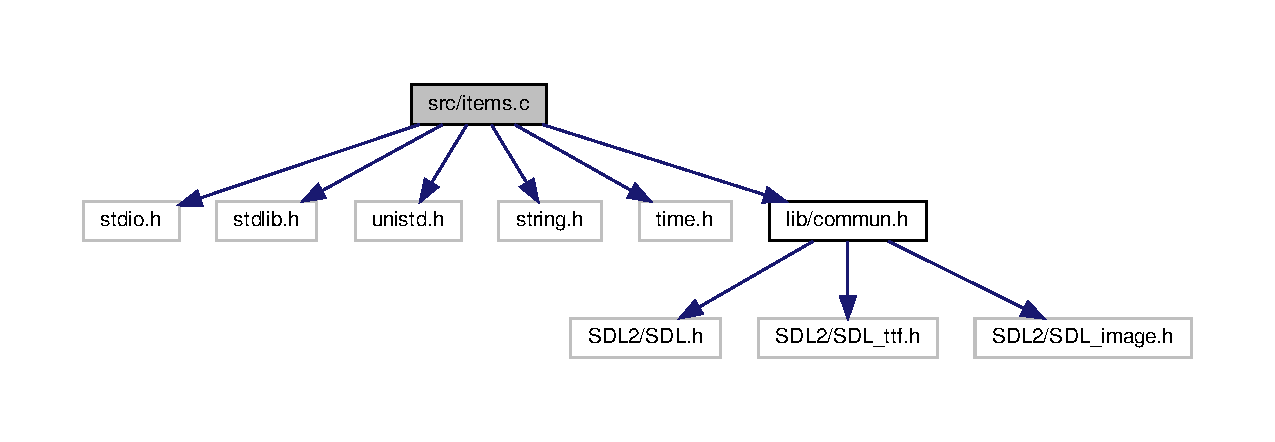
\includegraphics[width=350pt]{items_8c__incl}
\end{center}
\end{figure}
\subsection*{Fonctions}
\begin{DoxyCompactItemize}
\item 
\mbox{\Hypertarget{items_8c_ad37eb49f35a18814ef964030603d0ab8}\label{items_8c_ad37eb49f35a18814ef964030603d0ab8}} 
item\+\_\+t $\ast$ {\bfseries creer\+\_\+item} (char $\ast$chaine, type\+\_\+t type, int attack0, int attack1, int attack2, int hitchance0, int hitchance1, int hitchance2, float defense, int equipable, int pc\+\_\+nature, int pc\+\_\+urban, int pc\+\_\+military)
\item 
int \hyperlink{items_8c_a6bfcbccc63814dc4ba0642b7872e8681}{creation\+\_\+tab\+\_\+item} (item\+\_\+t $\ast$Tab\+\_\+\+Items, int $\ast$nb\+\_\+items)
\begin{DoxyCompactList}\small\item\em Récupère les items du fichier \textquotesingle{}items.\+csv\textquotesingle{} et les stocke dans le tableau passé en paramètres. \end{DoxyCompactList}\item 
void \hyperlink{items_8c_af20ce6de62a477209830e29feb783aa1}{display\+\_\+item} (item\+\_\+t item)
\begin{DoxyCompactList}\small\item\em Affiche toutes les caractéristiques d\textquotesingle{}un item (nom, type, valeur d\textquotesingle{}attaque si arme, valeur de défense si armure, équipable ou non, pc\+\_\+nature, pc\+\_\+urban, pc\+\_\+military) \end{DoxyCompactList}\end{DoxyCompactItemize}


\subsection{Description détaillée}
Fonctions relatives aux items. 

\begin{DoxyAuthor}{Auteur}
Mathilde Mottay, Anaïs Mottier, Clément Mainguy, Moustapha Tsamarayev 
\end{DoxyAuthor}
\begin{DoxyVersion}{Version}
1.\+0 
\end{DoxyVersion}
\begin{DoxyDate}{Date}
2020 
\end{DoxyDate}


\subsection{Documentation des fonctions}
\mbox{\Hypertarget{items_8c_a6bfcbccc63814dc4ba0642b7872e8681}\label{items_8c_a6bfcbccc63814dc4ba0642b7872e8681}} 
\index{items.\+c@{items.\+c}!creation\+\_\+tab\+\_\+item@{creation\+\_\+tab\+\_\+item}}
\index{creation\+\_\+tab\+\_\+item@{creation\+\_\+tab\+\_\+item}!items.\+c@{items.\+c}}
\subsubsection{\texorpdfstring{creation\+\_\+tab\+\_\+item()}{creation\_tab\_item()}}
{\footnotesize\ttfamily int creation\+\_\+tab\+\_\+item (\begin{DoxyParamCaption}\item[{item\+\_\+t $\ast$}]{Tab\+\_\+\+Items,  }\item[{int $\ast$}]{nb\+\_\+items }\end{DoxyParamCaption})}



Récupère les items du fichier \textquotesingle{}items.\+csv\textquotesingle{} et les stocke dans le tableau passé en paramètres. 

Affiche un message d\textquotesingle{}erreur si fichier \textquotesingle{}items.\+csv\textquotesingle{} non trouvé 
\begin{DoxyParams}{Paramètres}
{\em char} & $\ast$ Tab\+\_\+\+Items \\
\hline
{\em int} & $\ast$ nb\+\_\+items \\
\hline
\end{DoxyParams}
\begin{DoxyReturn}{Renvoie}
Un {\itshape int} \+: 1 si création des items réalisée avec succès. 0 sinon. 
\end{DoxyReturn}
\mbox{\Hypertarget{items_8c_af20ce6de62a477209830e29feb783aa1}\label{items_8c_af20ce6de62a477209830e29feb783aa1}} 
\index{items.\+c@{items.\+c}!display\+\_\+item@{display\+\_\+item}}
\index{display\+\_\+item@{display\+\_\+item}!items.\+c@{items.\+c}}
\subsubsection{\texorpdfstring{display\+\_\+item()}{display\_item()}}
{\footnotesize\ttfamily void display\+\_\+item (\begin{DoxyParamCaption}\item[{item\+\_\+t}]{item }\end{DoxyParamCaption})}



Affiche toutes les caractéristiques d\textquotesingle{}un item (nom, type, valeur d\textquotesingle{}attaque si arme, valeur de défense si armure, équipable ou non, pc\+\_\+nature, pc\+\_\+urban, pc\+\_\+military) 


\begin{DoxyParams}{Paramètres}
{\em item\+\_\+t} & item \\
\hline
\end{DoxyParams}
\begin{DoxyReturn}{Renvoie}
Rien 
\end{DoxyReturn}

\hypertarget{menu_8c}{}\section{Référence du fichier src/menu.c}
\label{menu_8c}\index{src/menu.\+c@{src/menu.\+c}}


M\+E\+NU P\+R\+I\+N\+C\+I\+P\+AL.  


{\ttfamily \#include $<$stdio.\+h$>$}\newline
{\ttfamily \#include $<$stdlib.\+h$>$}\newline
{\ttfamily \#include $<$time.\+h$>$}\newline
{\ttfamily \#include $<$unistd.\+h$>$}\newline
{\ttfamily \#include \char`\"{}lib/structure.\+h\char`\"{}}\newline
Graphe des dépendances par inclusion de menu.\+c\+:\nopagebreak
\begin{figure}[H]
\begin{center}
\leavevmode
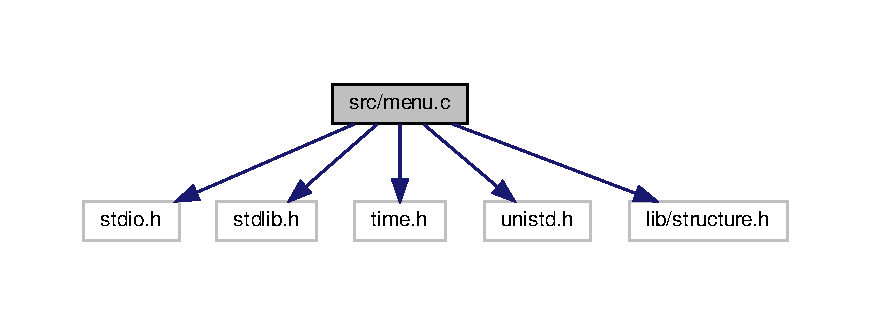
\includegraphics[width=350pt]{menu_8c__incl}
\end{center}
\end{figure}
\subsection*{Fonctions}
\begin{DoxyCompactItemize}
\item 
int \hyperlink{menu_8c_ae66f6b31b5ad750f1fe042a706a4e3d4}{main} ()
\begin{DoxyCompactList}\small\item\em Programme / Menu principal. \end{DoxyCompactList}\end{DoxyCompactItemize}


\subsection{Description détaillée}
M\+E\+NU P\+R\+I\+N\+C\+I\+P\+AL. 

\begin{DoxyAuthor}{Auteur}
Mathilde Mottay, Anaïs Mottier, Clément Mainguy, Moustapha Tsamarayev 
\end{DoxyAuthor}
\begin{DoxyVersion}{Version}
1.\+0 
\end{DoxyVersion}
\begin{DoxyDate}{Date}
2020 
\end{DoxyDate}


\subsection{Documentation des fonctions}
\mbox{\Hypertarget{menu_8c_ae66f6b31b5ad750f1fe042a706a4e3d4}\label{menu_8c_ae66f6b31b5ad750f1fe042a706a4e3d4}} 
\index{menu.\+c@{menu.\+c}!main@{main}}
\index{main@{main}!menu.\+c@{menu.\+c}}
\subsubsection{\texorpdfstring{main()}{main()}}
{\footnotesize\ttfamily int main (\begin{DoxyParamCaption}{ }\end{DoxyParamCaption})}



Programme / Menu principal. 


\begin{DoxyEnumerate}
\item Fouillez la zone
\item Gérer l\textquotesingle{}inventaire
\item Gérer l\textquotesingle{}équipement
\item Se déplacer ailleurs
\item Pêcher
\item Regarder la carte (carte nécessaire)
\item Se reposer et guérir
\item Fin du tour
\item Sauvegarder le jeu et quitter
\item Aide \begin{DoxyReturn}{Renvoie}
Rien 
\end{DoxyReturn}

\end{DoxyEnumerate}
\hypertarget{move_8c}{}\section{Référence du fichier src/move.c}
\label{move_8c}\index{src/move.\+c@{src/move.\+c}}


Déplacement du joueur.  


{\ttfamily \#include $<$stdio.\+h$>$}\newline
{\ttfamily \#include $<$stdlib.\+h$>$}\newline
{\ttfamily \#include $<$time.\+h$>$}\newline
{\ttfamily \#include $<$unistd.\+h$>$}\newline
{\ttfamily \#include \char`\"{}lib/commun.\+h\char`\"{}}\newline
Graphe des dépendances par inclusion de move.\+c\+:
\nopagebreak
\begin{figure}[H]
\begin{center}
\leavevmode
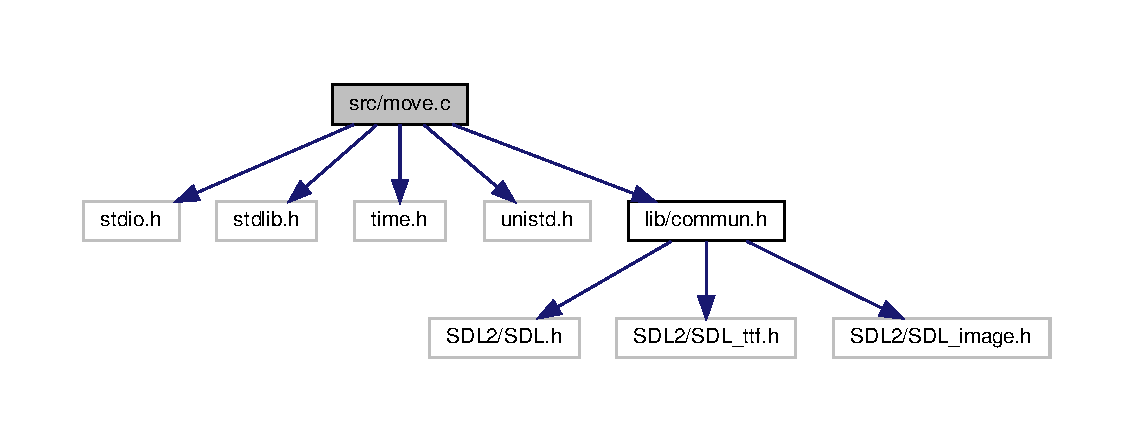
\includegraphics[width=350pt]{move_8c__incl}
\end{center}
\end{figure}
\subsection*{Fonctions}
\begin{DoxyCompactItemize}
\item 
int \hyperlink{move_8c_aaad16c14a2221260ca0a7b633c2991ae}{move\+\_\+lose\+\_\+pa} (\hyperlink{commun_8h_a86b2798c02561aa7def13bc6565d7290}{hex\+\_\+t} type\+\_\+hexa)
\begin{DoxyCompactList}\small\item\em Calcule le nombre de points d\textquotesingle{}action nécessaires pour se déplacer dans le type d\textquotesingle{}hexagone passé en paramètre. \end{DoxyCompactList}\item 
void \hyperlink{move_8c_a8810aae2a102048ffb6d87f85d4aa226}{look\+\_\+around} (int i, int j, \hyperlink{structcell__t}{cell\+\_\+t} map\mbox{[}\hyperlink{commun_8h_af316c33cc298530f245e8b55330e86b5}{D}\mbox{]}\mbox{[}\hyperlink{commun_8h_af316c33cc298530f245e8b55330e86b5}{D}\mbox{]})
\begin{DoxyCompactList}\small\item\em Affiche une vue des 8 hexagones qui entourent le joueur et les codes pour choisir où se déplacer. \end{DoxyCompactList}\item 
void \hyperlink{move_8c_ac9fb4bd5a16513e8faf4bf23dcb3d2bf}{move} (\hyperlink{structperso__t}{perso\+\_\+t} $\ast$player, \hyperlink{structcell__t}{cell\+\_\+t} map\mbox{[}\hyperlink{commun_8h_af316c33cc298530f245e8b55330e86b5}{D}\mbox{]}\mbox{[}\hyperlink{commun_8h_af316c33cc298530f245e8b55330e86b5}{D}\mbox{]})
\begin{DoxyCompactList}\small\item\em Déplace le joueur où il le souhaite, si cela est possible (conditions \+: coordonnées valides et assez de points d\textquotesingle{}action) \end{DoxyCompactList}\item 
void \hyperlink{move_8c_a27e09d79b0c98039d2d6f07dd485ccc0}{random\+\_\+move} (\hyperlink{structperso__t}{perso\+\_\+t} $\ast$player, \hyperlink{structcell__t}{cell\+\_\+t} map\mbox{[}\hyperlink{commun_8h_af316c33cc298530f245e8b55330e86b5}{D}\mbox{]}\mbox{[}\hyperlink{commun_8h_af316c33cc298530f245e8b55330e86b5}{D}\mbox{]})
\begin{DoxyCompactList}\small\item\em Déplace aléatoirement le joueur sur un des hexagones qui l\textquotesingle{}entoure. \end{DoxyCompactList}\end{DoxyCompactItemize}


\subsection{Description détaillée}
Déplacement du joueur. 

\begin{DoxyAuthor}{Auteur}
Mathilde Mottay, Anaïs Mottier, Clément Mainguy, Moustapha Tsamarayev 
\end{DoxyAuthor}
\begin{DoxyVersion}{Version}
1.\+0 
\end{DoxyVersion}
\begin{DoxyDate}{Date}
2020 
\end{DoxyDate}


\subsection{Documentation des fonctions}
\mbox{\Hypertarget{move_8c_a8810aae2a102048ffb6d87f85d4aa226}\label{move_8c_a8810aae2a102048ffb6d87f85d4aa226}} 
\index{move.\+c@{move.\+c}!look\+\_\+around@{look\+\_\+around}}
\index{look\+\_\+around@{look\+\_\+around}!move.\+c@{move.\+c}}
\subsubsection{\texorpdfstring{look\+\_\+around()}{look\_around()}}
{\footnotesize\ttfamily void look\+\_\+around (\begin{DoxyParamCaption}\item[{int}]{i,  }\item[{int}]{j,  }\item[{\hyperlink{structcell__t}{cell\+\_\+t}}]{map\mbox{[}\+D\mbox{]}\mbox{[}\+D\mbox{]} }\end{DoxyParamCaption})}



Affiche une vue des 8 hexagones qui entourent le joueur et les codes pour choisir où se déplacer. 


\begin{DoxyParams}{Paramètres}
{\em i} & Coordonnée ligne de l\textquotesingle{}hexagone sur lequel le joueur se trouve \\
\hline
{\em j} & Coordonnée colonne de l\textquotesingle{}hexagone sur lequel le joueur se trouve \\
\hline
{\em map\mbox{[}\+D\mbox{]}\mbox{[}\+D\mbox{]}} & Matrice de la carte \\
\hline
\end{DoxyParams}
\begin{DoxyReturn}{Renvoie}
Rien 
\end{DoxyReturn}
\mbox{\Hypertarget{move_8c_ac9fb4bd5a16513e8faf4bf23dcb3d2bf}\label{move_8c_ac9fb4bd5a16513e8faf4bf23dcb3d2bf}} 
\index{move.\+c@{move.\+c}!move@{move}}
\index{move@{move}!move.\+c@{move.\+c}}
\subsubsection{\texorpdfstring{move()}{move()}}
{\footnotesize\ttfamily void move (\begin{DoxyParamCaption}\item[{\hyperlink{structperso__t}{perso\+\_\+t} $\ast$}]{player,  }\item[{\hyperlink{structcell__t}{cell\+\_\+t}}]{map\mbox{[}\+D\mbox{]}\mbox{[}\+D\mbox{]} }\end{DoxyParamCaption})}



Déplace le joueur où il le souhaite, si cela est possible (conditions \+: coordonnées valides et assez de points d\textquotesingle{}action) 


\begin{DoxyParams}{Paramètres}
{\em player} & Pointeur sur un objet de type \hyperlink{structperso__t}{perso\+\_\+t} correspondant au joueur \\
\hline
{\em map\mbox{[}\+D\mbox{]}\mbox{[}\+D\mbox{]}} & Matrice de la carte \\
\hline
\end{DoxyParams}
\begin{DoxyReturn}{Renvoie}
Rien 
\end{DoxyReturn}
\mbox{\Hypertarget{move_8c_aaad16c14a2221260ca0a7b633c2991ae}\label{move_8c_aaad16c14a2221260ca0a7b633c2991ae}} 
\index{move.\+c@{move.\+c}!move\+\_\+lose\+\_\+pa@{move\+\_\+lose\+\_\+pa}}
\index{move\+\_\+lose\+\_\+pa@{move\+\_\+lose\+\_\+pa}!move.\+c@{move.\+c}}
\subsubsection{\texorpdfstring{move\+\_\+lose\+\_\+pa()}{move\_lose\_pa()}}
{\footnotesize\ttfamily int move\+\_\+lose\+\_\+pa (\begin{DoxyParamCaption}\item[{\hyperlink{commun_8h_a86b2798c02561aa7def13bc6565d7290}{hex\+\_\+t}}]{type\+\_\+hexa }\end{DoxyParamCaption})}



Calcule le nombre de points d\textquotesingle{}action nécessaires pour se déplacer dans le type d\textquotesingle{}hexagone passé en paramètre. 


\begin{DoxyParams}{Paramètres}
{\em type\+\_\+hexa} & Type de l\textquotesingle{}hexagone sur lequel le joueur souhaite se déplacer \\
\hline
\end{DoxyParams}
\begin{DoxyReturn}{Renvoie}
Un {\itshape int} représentant le nombre de points d\textquotesingle{}action nécessaires (prairie \+: 1, forêt \+: 2, ville \+: 1, lac \+: 2, camp militaire \+: 2, camp des bandits \+: 2, marché \+: 1, favela \+: 2, montagne \+: 3, frontière \+: 1, mer \+: 1, wasteland \+: 1) 
\end{DoxyReturn}
\mbox{\Hypertarget{move_8c_a27e09d79b0c98039d2d6f07dd485ccc0}\label{move_8c_a27e09d79b0c98039d2d6f07dd485ccc0}} 
\index{move.\+c@{move.\+c}!random\+\_\+move@{random\+\_\+move}}
\index{random\+\_\+move@{random\+\_\+move}!move.\+c@{move.\+c}}
\subsubsection{\texorpdfstring{random\+\_\+move()}{random\_move()}}
{\footnotesize\ttfamily void random\+\_\+move (\begin{DoxyParamCaption}\item[{\hyperlink{structperso__t}{perso\+\_\+t} $\ast$}]{player,  }\item[{\hyperlink{structcell__t}{cell\+\_\+t}}]{map\mbox{[}\+D\mbox{]}\mbox{[}\+D\mbox{]} }\end{DoxyParamCaption})}



Déplace aléatoirement le joueur sur un des hexagones qui l\textquotesingle{}entoure. 


\begin{DoxyParams}{Paramètres}
{\em player} & Pointeur sur un objet de type \hyperlink{structperso__t}{perso\+\_\+t} correspondant au joueur \\
\hline
{\em map\mbox{[}\+D\mbox{]}\mbox{[}\+D\mbox{]}} & Matrice de la carte \\
\hline
\end{DoxyParams}
\begin{DoxyReturn}{Renvoie}
Rien 
\end{DoxyReturn}

\hypertarget{perso_8c}{}\section{Référence du fichier src/perso.c}
\label{perso_8c}\index{src/perso.\+c@{src/perso.\+c}}


Fonctions relatives au joueur.  


{\ttfamily \#include $<$stdio.\+h$>$}\newline
{\ttfamily \#include $<$stdlib.\+h$>$}\newline
{\ttfamily \#include $<$string.\+h$>$}\newline
{\ttfamily \#include $<$time.\+h$>$}\newline
{\ttfamily \#include \char`\"{}lib/structure.\+h\char`\"{}}\newline
Graphe des dépendances par inclusion de perso.\+c\+:\nopagebreak
\begin{figure}[H]
\begin{center}
\leavevmode
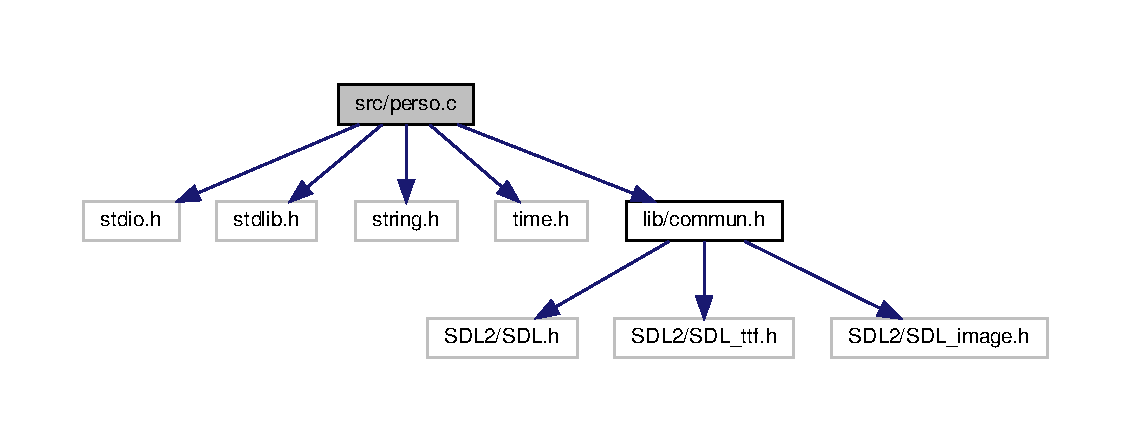
\includegraphics[width=350pt]{perso_8c__incl}
\end{center}
\end{figure}
\subsection*{Fonctions}
\begin{DoxyCompactItemize}
\item 
void \hyperlink{perso_8c_a0396d4741659c7486fe24a115e791d3b}{init\+\_\+player} (perso\+\_\+t $\ast$player)
\begin{DoxyCompactList}\small\item\em Initialise les paramètres du joueur quand il commence le jeu. \end{DoxyCompactList}\item 
void \hyperlink{perso_8c_abb56898d20ef15d05edb82a7dfbe8df9}{display\+\_\+player\+\_\+characteristics} (cell\+\_\+t map\mbox{[}D\mbox{]}\mbox{[}D\mbox{]}, perso\+\_\+t player)
\begin{DoxyCompactList}\small\item\em Affiche les paramètres du joueur (points de vie, points d\textquotesingle{}énergie, points d\textquotesingle{}action, position sur la carte, nombre de tours restants) \end{DoxyCompactList}\end{DoxyCompactItemize}


\subsection{Description détaillée}
Fonctions relatives au joueur. 

\begin{DoxyAuthor}{Auteur}
Mathilde Mottay, Anaïs Mottier, Clément Mainguy, Moustapha Tsamarayev 
\end{DoxyAuthor}
\begin{DoxyVersion}{Version}
1.\+0 
\end{DoxyVersion}
\begin{DoxyDate}{Date}
2020 
\end{DoxyDate}


\subsection{Documentation des fonctions}
\mbox{\Hypertarget{perso_8c_abb56898d20ef15d05edb82a7dfbe8df9}\label{perso_8c_abb56898d20ef15d05edb82a7dfbe8df9}} 
\index{perso.\+c@{perso.\+c}!display\+\_\+player\+\_\+characteristics@{display\+\_\+player\+\_\+characteristics}}
\index{display\+\_\+player\+\_\+characteristics@{display\+\_\+player\+\_\+characteristics}!perso.\+c@{perso.\+c}}
\subsubsection{\texorpdfstring{display\+\_\+player\+\_\+characteristics()}{display\_player\_characteristics()}}
{\footnotesize\ttfamily void display\+\_\+player\+\_\+characteristics (\begin{DoxyParamCaption}\item[{cell\+\_\+t}]{map\mbox{[}\+D\mbox{]}\mbox{[}\+D\mbox{]},  }\item[{perso\+\_\+t}]{player }\end{DoxyParamCaption})}



Affiche les paramètres du joueur (points de vie, points d\textquotesingle{}énergie, points d\textquotesingle{}action, position sur la carte, nombre de tours restants) 


\begin{DoxyParams}{Paramètres}
{\em cell\+\_\+t} & map\mbox{[}D\mbox{]}\mbox{[}D\mbox{]} \\
\hline
{\em perso\+\_\+t} & player \\
\hline
\end{DoxyParams}
\begin{DoxyReturn}{Renvoie}
Rien 
\end{DoxyReturn}
\mbox{\Hypertarget{perso_8c_a0396d4741659c7486fe24a115e791d3b}\label{perso_8c_a0396d4741659c7486fe24a115e791d3b}} 
\index{perso.\+c@{perso.\+c}!init\+\_\+player@{init\+\_\+player}}
\index{init\+\_\+player@{init\+\_\+player}!perso.\+c@{perso.\+c}}
\subsubsection{\texorpdfstring{init\+\_\+player()}{init\_player()}}
{\footnotesize\ttfamily void init\+\_\+player (\begin{DoxyParamCaption}\item[{perso\+\_\+t $\ast$}]{player }\end{DoxyParamCaption})}



Initialise les paramètres du joueur quand il commence le jeu. 


\begin{DoxyParams}{Paramètres}
{\em perso\+\_\+t} & $\ast$ player \\
\hline
\end{DoxyParams}
\begin{DoxyReturn}{Renvoie}
Rien 
\end{DoxyReturn}

\hypertarget{quete__soin_8c}{}\section{Référence du fichier src/quete\+\_\+soin.c}
\label{quete__soin_8c}\index{src/quete\+\_\+soin.\+c@{src/quete\+\_\+soin.\+c}}


Fonctions utilisees dans la quete \char`\"{}soin\char`\"{}.  


{\ttfamily \#include $<$stdio.\+h$>$}\newline
{\ttfamily \#include $<$stdlib.\+h$>$}\newline
{\ttfamily \#include $<$string.\+h$>$}\newline
{\ttfamily \#include $<$time.\+h$>$}\newline
{\ttfamily \#include $<$unistd.\+h$>$}\newline
{\ttfamily \#include \char`\"{}lib/structure.\+h\char`\"{}}\newline
Graphe des dépendances par inclusion de quete\+\_\+soin.\+c\+:\nopagebreak
\begin{figure}[H]
\begin{center}
\leavevmode
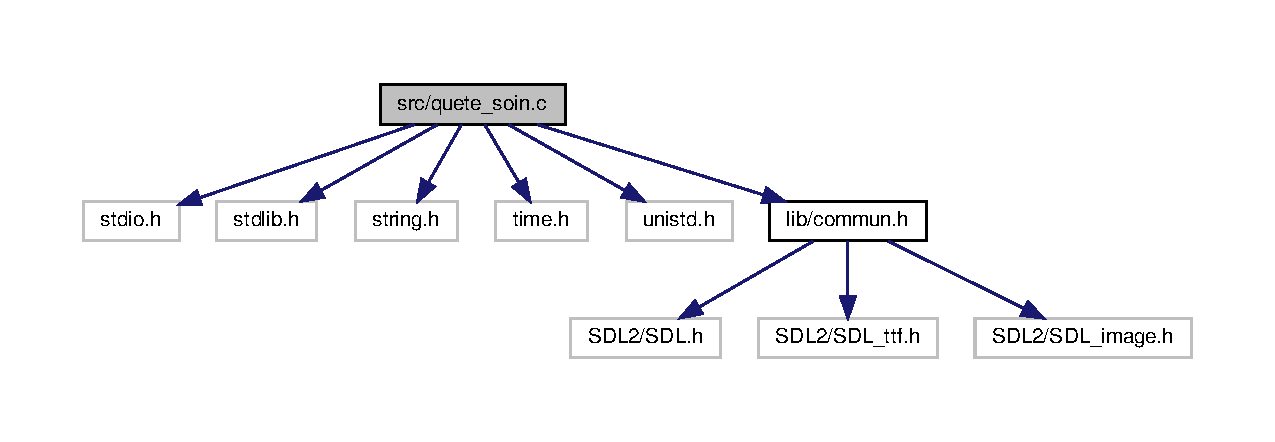
\includegraphics[width=350pt]{quete__soin_8c__incl}
\end{center}
\end{figure}
\subsection*{Fonctions}
\begin{DoxyCompactItemize}
\item 
npc\+\_\+t $\ast$ \hyperlink{quete__soin_8c_a7d129df227c67d85999f25b33eba672a}{init\+\_\+npc\+\_\+quete} (item\+\_\+t $\ast$Tab\+\_\+\+Items, int pers)
\begin{DoxyCompactList}\small\item\em Initialisation du personnage de l\textquotesingle{}homme bless�. \end{DoxyCompactList}\item 
int \hyperlink{quete__soin_8c_a1a1d9de9f3c8856b27220cc68879f6a6}{ajout\+\_\+item\+\_\+blesse} (perso\+\_\+t $\ast$player, npc\+\_\+t $\ast$homme, int item)
\begin{DoxyCompactList}\small\item\em Ajouter un item appartenant a un npc a l\textquotesingle{}inventaire du joueur. \end{DoxyCompactList}\item 
int \hyperlink{quete__soin_8c_a24a3e3e264884fa86338b8f5b38b01f6}{ajout\+\_\+pass\+\_\+card} (perso\+\_\+t $\ast$player, item\+\_\+t $\ast$pass\+\_\+card)
\begin{DoxyCompactList}\small\item\em Ajouter l\textquotesingle{}item pass\+\_\+card a l\textquotesingle{}inventaire du joueur. \end{DoxyCompactList}\item 
int \hyperlink{quete__soin_8c_a287944284de4bdcd2d3c3178ebd79adf}{menu\+\_\+choix\+\_\+ajout\+\_\+item} (perso\+\_\+t $\ast$player, item\+\_\+t $\ast$pass\+\_\+card, npc\+\_\+t $\ast$homme)
\begin{DoxyCompactList}\small\item\em Menu permettant au joueur de choisir quel item il souhaite ajoute a son inventaire;. \end{DoxyCompactList}\item 
int \hyperlink{quete__soin_8c_a724b2929f9e38cfa79e5caa45e982a42}{recup\+\_\+1item\+\_\+vole} (perso\+\_\+t $\ast$player, int nb\+\_\+items\+\_\+vole, npc\+\_\+t $\ast$homme, item\+\_\+t $\ast$pass\+\_\+card)
\begin{DoxyCompactList}\small\item\em Deroulement de la quete \char`\"{}soin\char`\"{} quand le joueur souhaite voler des items du npc et qu\textquotesingle{}il n\textquotesingle{}en trouve qu\textquotesingle{}un seul sur l\textquotesingle{}homme \+: le pass card. \end{DoxyCompactList}\item 
int \hyperlink{quete__soin_8c_ae3700bdf87b41634c1e8c4b3ad8a9cf7}{recup\+\_\+2items\+\_\+vole} (perso\+\_\+t $\ast$player, int nb\+\_\+items\+\_\+vole, npc\+\_\+t $\ast$homme, item\+\_\+t $\ast$pass\+\_\+card)
\begin{DoxyCompactList}\small\item\em Deroulement de la quete \char`\"{}soin\char`\"{} quand le joueur souhaite voler des items du npc et qu\textquotesingle{}il en trouve 2 sur l\textquotesingle{}homme. \end{DoxyCompactList}\item 
int \hyperlink{quete__soin_8c_ae8268170d69e016c56e99b048fce5ebf}{recup\+\_\+3items\+\_\+vole} (perso\+\_\+t $\ast$player, int nb\+\_\+items\+\_\+vole, npc\+\_\+t $\ast$homme, item\+\_\+t $\ast$pass\+\_\+card)
\begin{DoxyCompactList}\small\item\em Deroulement de la quete \char`\"{}soin\char`\"{} quand le joueur souhaite voler des items du npc et qu\textquotesingle{}il en trouve 3 sur l\textquotesingle{}homme. \end{DoxyCompactList}\item 
\mbox{\Hypertarget{quete__soin_8c_aef0b337811ec7b63569593e537d374c4}\label{quete__soin_8c_aef0b337811ec7b63569593e537d374c4}} 
int {\bfseries quete\+\_\+soin} (perso\+\_\+t $\ast$player, quete\+\_\+t $\ast$quete)
\end{DoxyCompactItemize}


\subsection{Description détaillée}
Fonctions utilisees dans la quete \char`\"{}soin\char`\"{}. 

\begin{DoxyAuthor}{Auteur}
Mathilde Mottay, Anais Mottier, Clement Mainguy, Moustapha Tsamarayev 
\end{DoxyAuthor}
\begin{DoxyVersion}{Version}

\end{DoxyVersion}
\begin{DoxyDate}{Date}
2020 
\end{DoxyDate}


\subsection{Documentation des fonctions}
\mbox{\Hypertarget{quete__soin_8c_a1a1d9de9f3c8856b27220cc68879f6a6}\label{quete__soin_8c_a1a1d9de9f3c8856b27220cc68879f6a6}} 
\index{quete\+\_\+soin.\+c@{quete\+\_\+soin.\+c}!ajout\+\_\+item\+\_\+blesse@{ajout\+\_\+item\+\_\+blesse}}
\index{ajout\+\_\+item\+\_\+blesse@{ajout\+\_\+item\+\_\+blesse}!quete\+\_\+soin.\+c@{quete\+\_\+soin.\+c}}
\subsubsection{\texorpdfstring{ajout\+\_\+item\+\_\+blesse()}{ajout\_item\_blesse()}}
{\footnotesize\ttfamily int ajout\+\_\+item\+\_\+blesse (\begin{DoxyParamCaption}\item[{perso\+\_\+t $\ast$}]{player,  }\item[{npc\+\_\+t $\ast$}]{homme,  }\item[{int}]{item }\end{DoxyParamCaption})}



Ajouter un item appartenant a un npc a l\textquotesingle{}inventaire du joueur. 


\begin{DoxyParams}{Paramètres}
{\em perso\+\_\+t} & $\ast$ player \\
\hline
{\em npc\+\_\+t} & $\ast$ homme \\
\hline
{\em int} & item \\
\hline
\end{DoxyParams}
\begin{DoxyReturn}{Renvoie}
Retourne un {\itshape int} \+: 0 si le jeu continue, -\/1 si probleme lors de la quete. 
\end{DoxyReturn}
\mbox{\Hypertarget{quete__soin_8c_a24a3e3e264884fa86338b8f5b38b01f6}\label{quete__soin_8c_a24a3e3e264884fa86338b8f5b38b01f6}} 
\index{quete\+\_\+soin.\+c@{quete\+\_\+soin.\+c}!ajout\+\_\+pass\+\_\+card@{ajout\+\_\+pass\+\_\+card}}
\index{ajout\+\_\+pass\+\_\+card@{ajout\+\_\+pass\+\_\+card}!quete\+\_\+soin.\+c@{quete\+\_\+soin.\+c}}
\subsubsection{\texorpdfstring{ajout\+\_\+pass\+\_\+card()}{ajout\_pass\_card()}}
{\footnotesize\ttfamily int ajout\+\_\+pass\+\_\+card (\begin{DoxyParamCaption}\item[{perso\+\_\+t $\ast$}]{player,  }\item[{item\+\_\+t $\ast$}]{pass\+\_\+card }\end{DoxyParamCaption})}



Ajouter l\textquotesingle{}item pass\+\_\+card a l\textquotesingle{}inventaire du joueur. 


\begin{DoxyParams}{Paramètres}
{\em perso\+\_\+t} & $\ast$ player \\
\hline
{\em item\+\_\+t} & $\ast$ pass\+\_\+card \\
\hline
\end{DoxyParams}
\begin{DoxyReturn}{Renvoie}
Retourne un {\itshape int} \+: 0 si le jeu continue, -\/1 si probleme lors de la quete. 
\end{DoxyReturn}
\mbox{\Hypertarget{quete__soin_8c_a7d129df227c67d85999f25b33eba672a}\label{quete__soin_8c_a7d129df227c67d85999f25b33eba672a}} 
\index{quete\+\_\+soin.\+c@{quete\+\_\+soin.\+c}!init\+\_\+npc\+\_\+quete@{init\+\_\+npc\+\_\+quete}}
\index{init\+\_\+npc\+\_\+quete@{init\+\_\+npc\+\_\+quete}!quete\+\_\+soin.\+c@{quete\+\_\+soin.\+c}}
\subsubsection{\texorpdfstring{init\+\_\+npc\+\_\+quete()}{init\_npc\_quete()}}
{\footnotesize\ttfamily npc\+\_\+t $\ast$ init\+\_\+npc\+\_\+quete (\begin{DoxyParamCaption}\item[{item\+\_\+t $\ast$}]{Tab\+\_\+\+Items,  }\item[{int}]{pers }\end{DoxyParamCaption})}



Initialisation du personnage de l\textquotesingle{}homme bless�. 

L\textquotesingle{}initialisation est differente en fonction du \char`\"{}metier\char`\"{} de l\textquotesingle{}homme \+: soldat, policier. Il n\textquotesingle{}aura pas la meme arme mais aura la meme armure. 
\begin{DoxyParams}{Paramètres}
{\em item\+\_\+t} & $\ast$ Tab\+\_\+\+Items \\
\hline
{\em int} & pers \\
\hline
\end{DoxyParams}
\begin{DoxyReturn}{Renvoie}
Un pointeur (npc\+\_\+t) sur le npc cree 
\end{DoxyReturn}
\mbox{\Hypertarget{quete__soin_8c_a287944284de4bdcd2d3c3178ebd79adf}\label{quete__soin_8c_a287944284de4bdcd2d3c3178ebd79adf}} 
\index{quete\+\_\+soin.\+c@{quete\+\_\+soin.\+c}!menu\+\_\+choix\+\_\+ajout\+\_\+item@{menu\+\_\+choix\+\_\+ajout\+\_\+item}}
\index{menu\+\_\+choix\+\_\+ajout\+\_\+item@{menu\+\_\+choix\+\_\+ajout\+\_\+item}!quete\+\_\+soin.\+c@{quete\+\_\+soin.\+c}}
\subsubsection{\texorpdfstring{menu\+\_\+choix\+\_\+ajout\+\_\+item()}{menu\_choix\_ajout\_item()}}
{\footnotesize\ttfamily int menu\+\_\+choix\+\_\+ajout\+\_\+item (\begin{DoxyParamCaption}\item[{perso\+\_\+t $\ast$}]{player,  }\item[{item\+\_\+t $\ast$}]{pass\+\_\+card,  }\item[{npc\+\_\+t $\ast$}]{homme }\end{DoxyParamCaption})}



Menu permettant au joueur de choisir quel item il souhaite ajoute a son inventaire;. 

Le joueur fait son choix et par la suite la fonction fait appel a une autre fonction (ajout\+\_\+item\+\_\+blesse, ajout\+\_\+pass\+\_\+card) qui ajoute l\textquotesingle{}item choisi 
\begin{DoxyParams}{Paramètres}
{\em perso\+\_\+t} & $\ast$ player \\
\hline
{\em item\+\_\+t} & $\ast$ pass\+\_\+card \\
\hline
{\em npc\+\_\+t} & $\ast$ homme \\
\hline
\end{DoxyParams}
\begin{DoxyReturn}{Renvoie}
Retourne un {\itshape int} \+: 0 si le jeu continue, -\/1 si probleme lors de la quete. 
\end{DoxyReturn}
\mbox{\Hypertarget{quete__soin_8c_a724b2929f9e38cfa79e5caa45e982a42}\label{quete__soin_8c_a724b2929f9e38cfa79e5caa45e982a42}} 
\index{quete\+\_\+soin.\+c@{quete\+\_\+soin.\+c}!recup\+\_\+1item\+\_\+vole@{recup\+\_\+1item\+\_\+vole}}
\index{recup\+\_\+1item\+\_\+vole@{recup\+\_\+1item\+\_\+vole}!quete\+\_\+soin.\+c@{quete\+\_\+soin.\+c}}
\subsubsection{\texorpdfstring{recup\+\_\+1item\+\_\+vole()}{recup\_1item\_vole()}}
{\footnotesize\ttfamily int recup\+\_\+1item\+\_\+vole (\begin{DoxyParamCaption}\item[{perso\+\_\+t $\ast$}]{player,  }\item[{int}]{nb\+\_\+items\+\_\+vole,  }\item[{npc\+\_\+t $\ast$}]{homme,  }\item[{item\+\_\+t $\ast$}]{pass\+\_\+card }\end{DoxyParamCaption})}



Deroulement de la quete \char`\"{}soin\char`\"{} quand le joueur souhaite voler des items du npc et qu\textquotesingle{}il n\textquotesingle{}en trouve qu\textquotesingle{}un seul sur l\textquotesingle{}homme \+: le pass card. 

Le joueur fait son choix entre voler le pass\+\_\+card l\textquotesingle{}ajouter a son inventaire ou non. 
\begin{DoxyParams}{Paramètres}
{\em perso\+\_\+t} & $\ast$ player \\
\hline
{\em int} & nb\+\_\+items\+\_\+vole \\
\hline
{\em npc\+\_\+t} & $\ast$ homme \\
\hline
{\em item\+\_\+t} & $\ast$ pass\+\_\+card \\
\hline
\end{DoxyParams}
\begin{DoxyReturn}{Renvoie}
Retourne un {\itshape int} \+: 0 si le jeu continue, -\/1 si probleme lors de la quete. 
\end{DoxyReturn}
\mbox{\Hypertarget{quete__soin_8c_ae3700bdf87b41634c1e8c4b3ad8a9cf7}\label{quete__soin_8c_ae3700bdf87b41634c1e8c4b3ad8a9cf7}} 
\index{quete\+\_\+soin.\+c@{quete\+\_\+soin.\+c}!recup\+\_\+2items\+\_\+vole@{recup\+\_\+2items\+\_\+vole}}
\index{recup\+\_\+2items\+\_\+vole@{recup\+\_\+2items\+\_\+vole}!quete\+\_\+soin.\+c@{quete\+\_\+soin.\+c}}
\subsubsection{\texorpdfstring{recup\+\_\+2items\+\_\+vole()}{recup\_2items\_vole()}}
{\footnotesize\ttfamily int recup\+\_\+2items\+\_\+vole (\begin{DoxyParamCaption}\item[{perso\+\_\+t $\ast$}]{player,  }\item[{int}]{nb\+\_\+items\+\_\+vole,  }\item[{npc\+\_\+t $\ast$}]{homme,  }\item[{item\+\_\+t $\ast$}]{pass\+\_\+card }\end{DoxyParamCaption})}



Deroulement de la quete \char`\"{}soin\char`\"{} quand le joueur souhaite voler des items du npc et qu\textquotesingle{}il en trouve 2 sur l\textquotesingle{}homme. 

Le pass\+\_\+card est obligatoirement trouve, le deuxieme item est soit l\textquotesingle{}arme ou l\textquotesingle{}armure du npc. Le joueur fait son choix entre voler 1 ou 2 item(s) et le/les ajouter a son inventaire ou ne rien voler. 
\begin{DoxyParams}{Paramètres}
{\em perso\+\_\+t} & $\ast$ player \\
\hline
{\em int} & nb\+\_\+items\+\_\+vole \\
\hline
{\em npc\+\_\+t} & $\ast$ homme \\
\hline
{\em item\+\_\+t} & $\ast$ pass\+\_\+card \\
\hline
\end{DoxyParams}
\begin{DoxyReturn}{Renvoie}
Retourne un {\itshape int} \+: 0 si le jeu continue, -\/1 si probleme lors de la quete. 
\end{DoxyReturn}
\mbox{\Hypertarget{quete__soin_8c_ae8268170d69e016c56e99b048fce5ebf}\label{quete__soin_8c_ae8268170d69e016c56e99b048fce5ebf}} 
\index{quete\+\_\+soin.\+c@{quete\+\_\+soin.\+c}!recup\+\_\+3items\+\_\+vole@{recup\+\_\+3items\+\_\+vole}}
\index{recup\+\_\+3items\+\_\+vole@{recup\+\_\+3items\+\_\+vole}!quete\+\_\+soin.\+c@{quete\+\_\+soin.\+c}}
\subsubsection{\texorpdfstring{recup\+\_\+3items\+\_\+vole()}{recup\_3items\_vole()}}
{\footnotesize\ttfamily int recup\+\_\+3items\+\_\+vole (\begin{DoxyParamCaption}\item[{perso\+\_\+t $\ast$}]{player,  }\item[{int}]{nb\+\_\+items\+\_\+vole,  }\item[{npc\+\_\+t $\ast$}]{homme,  }\item[{item\+\_\+t $\ast$}]{pass\+\_\+card }\end{DoxyParamCaption})}



Deroulement de la quete \char`\"{}soin\char`\"{} quand le joueur souhaite voler des items du npc et qu\textquotesingle{}il en trouve 3 sur l\textquotesingle{}homme. 

Le joueur trouve le pass\+\_\+card, l\textquotesingle{}arme et l\textquotesingle{}armure du npc blesse. Il a le choix entre voler 1, 2 ou 3 item(s) et le/les ajouter a son inventaire ou ne rien voler. 
\begin{DoxyParams}{Paramètres}
{\em perso\+\_\+t} & $\ast$ player \\
\hline
{\em int} & nb\+\_\+items\+\_\+vole \\
\hline
{\em npc\+\_\+t} & $\ast$ homme \\
\hline
{\em item\+\_\+t} & $\ast$ pass\+\_\+card \\
\hline
\end{DoxyParams}
\begin{DoxyReturn}{Renvoie}
Retourne un {\itshape int} \+: 0 si le jeu continue, -\/1 si probleme lors de la quete. 
\end{DoxyReturn}

\hypertarget{quetes_8c}{}\section{Référence du fichier src/quetes.c}
\label{quetes_8c}\index{src/quetes.\+c@{src/quetes.\+c}}


Fonctions relatives aux quêtes du jeu (initialisation, lancement des quêtes) + 4 quêtes (montagne, frontière, bunker, bandits)  


{\ttfamily \#include $<$stdio.\+h$>$}\newline
{\ttfamily \#include $<$stdlib.\+h$>$}\newline
{\ttfamily \#include $<$string.\+h$>$}\newline
{\ttfamily \#include $<$time.\+h$>$}\newline
{\ttfamily \#include $<$unistd.\+h$>$}\newline
{\ttfamily \#include \char`\"{}lib/commun.\+h\char`\"{}}\newline
Graphe des dépendances par inclusion de quetes.\+c\+:\nopagebreak
\begin{figure}[H]
\begin{center}
\leavevmode
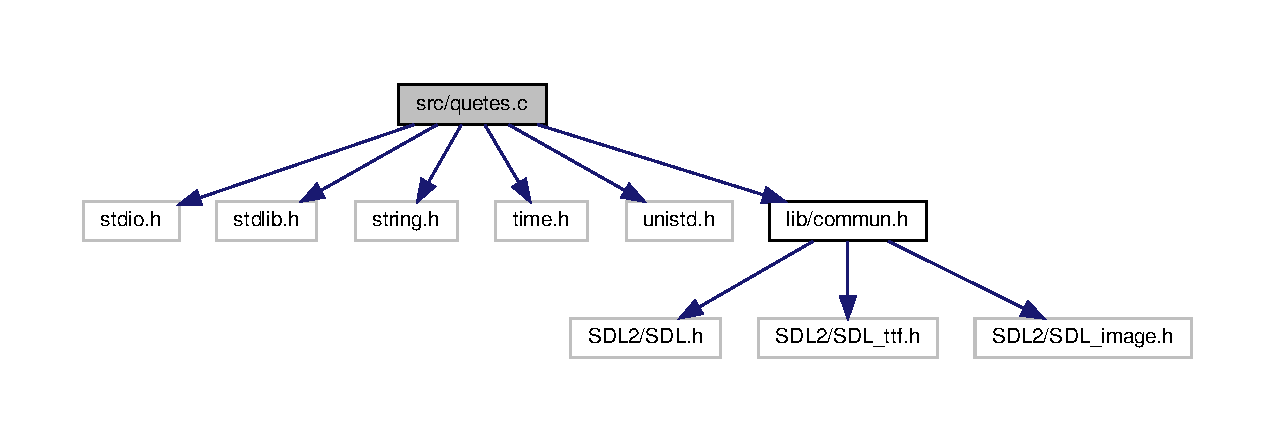
\includegraphics[width=350pt]{quetes_8c__incl}
\end{center}
\end{figure}
\subsection*{Fonctions}
\begin{DoxyCompactItemize}
\item 
int \hyperlink{quetes_8c_afd7728c9e6ae89e5932e641b54556aba}{exit\+\_\+game} ()
\begin{DoxyCompactList}\small\item\em Propose au joueur de quitter ou non la carte lorsqu\textquotesingle{}il vient de trouver la sortie. \end{DoxyCompactList}\item 
void \hyperlink{quetes_8c_a8467aba54144bfdead8e1a614e563e23}{informations\+\_\+quetes} (\hyperlink{structcell__t}{cell\+\_\+t} map\mbox{[}\hyperlink{commun_8h_af316c33cc298530f245e8b55330e86b5}{D}\mbox{]}\mbox{[}\hyperlink{commun_8h_af316c33cc298530f245e8b55330e86b5}{D}\mbox{]}, int quest\+\_\+map\mbox{[}6\mbox{]}\mbox{[}2\mbox{]}, \hyperlink{structquete__t}{quete\+\_\+t} quete)
\begin{DoxyCompactList}\small\item\em Affiche les informations des quêtes (coordonnées et états) \end{DoxyCompactList}\item 
void \hyperlink{quetes_8c_a88d64826f8f2155e0cbf149e18aa33c0}{init\+\_\+quete} (\hyperlink{structquete__t}{quete\+\_\+t} $\ast$quete, int quest\+\_\+map\mbox{[}6\mbox{]}\mbox{[}2\mbox{]}, \hyperlink{structitem__t}{item\+\_\+t} $\ast$Tab\+\_\+\+Items, int nb\+\_\+items\+\_\+available)
\begin{DoxyCompactList}\small\item\em Initialisation d\textquotesingle{}une variable de type \hyperlink{structquete__t}{quete\+\_\+t}. \end{DoxyCompactList}\item 
int \hyperlink{quetes_8c_adc1d91bf20af02d88470e87ff9bb9e8b}{quetes} (\hyperlink{structperso__t}{perso\+\_\+t} $\ast$player, \hyperlink{structcell__t}{cell\+\_\+t} map\mbox{[}\hyperlink{commun_8h_af316c33cc298530f245e8b55330e86b5}{D}\mbox{]}\mbox{[}\hyperlink{commun_8h_af316c33cc298530f245e8b55330e86b5}{D}\mbox{]}, int quest\+\_\+map\mbox{[}6\mbox{]}\mbox{[}2\mbox{]}, \hyperlink{structquete__t}{quete\+\_\+t} $\ast$quete, \hyperlink{structitem__t}{item\+\_\+t} $\ast$Tab\+\_\+\+Items, int nb\+\_\+items\+\_\+available)
\begin{DoxyCompactList}\small\item\em Récupère le numéro de la quête pour accéder à la quête correspondante. \end{DoxyCompactList}\item 
int \hyperlink{quetes_8c_ab993120c9273aa16f7789c84428d4ab9}{quete\+\_\+montagne} (\hyperlink{structperso__t}{perso\+\_\+t} $\ast$player, \hyperlink{structquete__t}{quete\+\_\+t} $\ast$quete)
\begin{DoxyCompactList}\small\item\em Accès à la quete \char`\"{}montagne\char`\"{}. \end{DoxyCompactList}\item 
int \hyperlink{quetes_8c_a7da8ac2437b193c7740204da24c04ae8}{quete\+\_\+frontiere} (\hyperlink{structperso__t}{perso\+\_\+t} $\ast$player, \hyperlink{structquete__t}{quete\+\_\+t} $\ast$quete)
\begin{DoxyCompactList}\small\item\em Accès à la quete \char`\"{}frontière\char`\"{}. \end{DoxyCompactList}\item 
int \hyperlink{quetes_8c_a266486f088d93c87682a8c3f1d130d64}{quete\+\_\+bunker} (\hyperlink{structperso__t}{perso\+\_\+t} $\ast$player, \hyperlink{structquete__t}{quete\+\_\+t} $\ast$quete)
\begin{DoxyCompactList}\small\item\em Accès à la quête \char`\"{}bunker\char`\"{}. \end{DoxyCompactList}\item 
int \hyperlink{quetes_8c_ae3a10faf1284038599e3098a8253ce43}{quete\+\_\+bandits} (\hyperlink{structperso__t}{perso\+\_\+t} $\ast$player, \hyperlink{structquete__t}{quete\+\_\+t} $\ast$quete, \hyperlink{structitem__t}{item\+\_\+t} $\ast$Tab\+\_\+\+Items, int nb\+\_\+items\+\_\+available, \hyperlink{structcell__t}{cell\+\_\+t} map\mbox{[}\hyperlink{commun_8h_af316c33cc298530f245e8b55330e86b5}{D}\mbox{]}\mbox{[}\hyperlink{commun_8h_af316c33cc298530f245e8b55330e86b5}{D}\mbox{]})
\begin{DoxyCompactList}\small\item\em Accès à la quete \char`\"{}bandits\char`\"{}. \end{DoxyCompactList}\end{DoxyCompactItemize}


\subsection{Description détaillée}
Fonctions relatives aux quêtes du jeu (initialisation, lancement des quêtes) + 4 quêtes (montagne, frontière, bunker, bandits) 

\begin{DoxyAuthor}{Auteur}
Mathilde Mottay, Anais Mottier, Clement Mainguy, Moustapha Tsamarayev 
\end{DoxyAuthor}
\begin{DoxyVersion}{Version}

\end{DoxyVersion}
\begin{DoxyDate}{Date}
2020 
\end{DoxyDate}


\subsection{Documentation des fonctions}
\mbox{\Hypertarget{quetes_8c_afd7728c9e6ae89e5932e641b54556aba}\label{quetes_8c_afd7728c9e6ae89e5932e641b54556aba}} 
\index{quetes.\+c@{quetes.\+c}!exit\+\_\+game@{exit\+\_\+game}}
\index{exit\+\_\+game@{exit\+\_\+game}!quetes.\+c@{quetes.\+c}}
\subsubsection{\texorpdfstring{exit\+\_\+game()}{exit\_game()}}
{\footnotesize\ttfamily int exit\+\_\+game (\begin{DoxyParamCaption}{ }\end{DoxyParamCaption})}



Propose au joueur de quitter ou non la carte lorsqu\textquotesingle{}il vient de trouver la sortie. 

\begin{DoxyReturn}{Renvoie}
Un {\itshape int} \+: 1 si le joueur décide de quitter la carte. 0 s\textquotesingle{}il décide de continuer l\textquotesingle{}aventure. 
\end{DoxyReturn}
\mbox{\Hypertarget{quetes_8c_a8467aba54144bfdead8e1a614e563e23}\label{quetes_8c_a8467aba54144bfdead8e1a614e563e23}} 
\index{quetes.\+c@{quetes.\+c}!informations\+\_\+quetes@{informations\+\_\+quetes}}
\index{informations\+\_\+quetes@{informations\+\_\+quetes}!quetes.\+c@{quetes.\+c}}
\subsubsection{\texorpdfstring{informations\+\_\+quetes()}{informations\_quetes()}}
{\footnotesize\ttfamily void informations\+\_\+quetes (\begin{DoxyParamCaption}\item[{\hyperlink{structcell__t}{cell\+\_\+t}}]{map\mbox{[}\+D\mbox{]}\mbox{[}\+D\mbox{]},  }\item[{int}]{quest\+\_\+map\mbox{[}6\mbox{]}\mbox{[}2\mbox{]},  }\item[{\hyperlink{structquete__t}{quete\+\_\+t}}]{quete }\end{DoxyParamCaption})}



Affiche les informations des quêtes (coordonnées et états) 


\begin{DoxyParams}{Paramètres}
{\em map\mbox{[}\+D\mbox{]}\mbox{[}\+D\mbox{]}} & Matrice de la carte \\
\hline
{\em quest\+\_\+map\mbox{[}6\mbox{]}\mbox{[}2\mbox{]}} & Matrice des coordonnées des quêtes \\
\hline
{\em quete} & Etat des quêtes \\
\hline
\end{DoxyParams}
\begin{DoxyReturn}{Renvoie}
Rien 
\end{DoxyReturn}
\mbox{\Hypertarget{quetes_8c_a88d64826f8f2155e0cbf149e18aa33c0}\label{quetes_8c_a88d64826f8f2155e0cbf149e18aa33c0}} 
\index{quetes.\+c@{quetes.\+c}!init\+\_\+quete@{init\+\_\+quete}}
\index{init\+\_\+quete@{init\+\_\+quete}!quetes.\+c@{quetes.\+c}}
\subsubsection{\texorpdfstring{init\+\_\+quete()}{init\_quete()}}
{\footnotesize\ttfamily void init\+\_\+quete (\begin{DoxyParamCaption}\item[{\hyperlink{structquete__t}{quete\+\_\+t} $\ast$}]{quete,  }\item[{int}]{quest\+\_\+map\mbox{[}6\mbox{]}\mbox{[}2\mbox{]},  }\item[{\hyperlink{structitem__t}{item\+\_\+t} $\ast$}]{Tab\+\_\+\+Items,  }\item[{int}]{nb\+\_\+items\+\_\+available }\end{DoxyParamCaption})}



Initialisation d\textquotesingle{}une variable de type \hyperlink{structquete__t}{quete\+\_\+t}. 


\begin{DoxyParams}{Paramètres}
{\em quete} & Pointeur sur un objet de type \hyperlink{structquete__t}{quete\+\_\+t} correspondant à l\textquotesingle{}état des quêtes \\
\hline
{\em quest\+\_\+map\mbox{[}6\mbox{]}\mbox{[}2\mbox{]}} & Matrice des coordonnées des quêtes \\
\hline
{\em Tab\+\_\+\+Items} & Tableau contenant tous les items disponibles dans le jeu \\
\hline
{\em nb\+\_\+items\+\_\+available} & Nombre d\textquotesingle{}items disponibles dans le jeu \\
\hline
\end{DoxyParams}
\begin{DoxyReturn}{Renvoie}
Rien 
\end{DoxyReturn}
\mbox{\Hypertarget{quetes_8c_ae3a10faf1284038599e3098a8253ce43}\label{quetes_8c_ae3a10faf1284038599e3098a8253ce43}} 
\index{quetes.\+c@{quetes.\+c}!quete\+\_\+bandits@{quete\+\_\+bandits}}
\index{quete\+\_\+bandits@{quete\+\_\+bandits}!quetes.\+c@{quetes.\+c}}
\subsubsection{\texorpdfstring{quete\+\_\+bandits()}{quete\_bandits()}}
{\footnotesize\ttfamily int quete\+\_\+bandits (\begin{DoxyParamCaption}\item[{\hyperlink{structperso__t}{perso\+\_\+t} $\ast$}]{player,  }\item[{\hyperlink{structquete__t}{quete\+\_\+t} $\ast$}]{quete,  }\item[{\hyperlink{structitem__t}{item\+\_\+t} $\ast$}]{Tab\+\_\+\+Items,  }\item[{int}]{nb\+\_\+items\+\_\+available,  }\item[{\hyperlink{structcell__t}{cell\+\_\+t}}]{map\mbox{[}\+D\mbox{]}\mbox{[}\+D\mbox{]} }\end{DoxyParamCaption})}



Accès à la quete \char`\"{}bandits\char`\"{}. 

Le joueur arrive sur un camp de bandits. Il a le choix entre fuir, attendre les hommes ou voler des items. Il en sort vivant ou mort. 
\begin{DoxyParams}{Paramètres}
{\em player} & Pointeur sur un objet de type \hyperlink{structperso__t}{perso\+\_\+t} correspondant au joueur \\
\hline
{\em quete} & Pointeur sur un objet de type \hyperlink{structquete__t}{quete\+\_\+t} correspondant à l\textquotesingle{}état des quêtes \\
\hline
{\em Tab\+\_\+\+Items} & Tableau contenant tous les items disponibles dans le jeu \\
\hline
{\em nb\+\_\+items\+\_\+available} & Nombre d\textquotesingle{}items disponibles dans le jeu \\
\hline
{\em map\mbox{[}\+D\mbox{]}\mbox{[}\+D\mbox{]}} & Matrice de la carte \\
\hline
\end{DoxyParams}
\begin{DoxyReturn}{Renvoie}
Retourne un {\itshape int} \+: 0 si le jeu continue, 1 si le jeu est fini et -\/1 si problème dans la quête. 
\end{DoxyReturn}
\mbox{\Hypertarget{quetes_8c_a266486f088d93c87682a8c3f1d130d64}\label{quetes_8c_a266486f088d93c87682a8c3f1d130d64}} 
\index{quetes.\+c@{quetes.\+c}!quete\+\_\+bunker@{quete\+\_\+bunker}}
\index{quete\+\_\+bunker@{quete\+\_\+bunker}!quetes.\+c@{quetes.\+c}}
\subsubsection{\texorpdfstring{quete\+\_\+bunker()}{quete\_bunker()}}
{\footnotesize\ttfamily void quete\+\_\+bunker (\begin{DoxyParamCaption}\item[{\hyperlink{structperso__t}{perso\+\_\+t} $\ast$}]{player,  }\item[{\hyperlink{structquete__t}{quete\+\_\+t} $\ast$}]{quete }\end{DoxyParamCaption})}



Accès à la quête \char`\"{}bunker\char`\"{}. 

Si le joueur possède le pass\+\_\+card, il aura le choix de rentrer dans le bunker ou non. Sinon il fait demi-\/tour. 
\begin{DoxyParams}{Paramètres}
{\em player} & Pointeur sur un objet de type \hyperlink{structperso__t}{perso\+\_\+t} correspondant au joueur \\
\hline
{\em quete} & Pointeur sur un objet de type \hyperlink{structquete__t}{quete\+\_\+t} correspondant à l\textquotesingle{}état des quêtes \\
\hline
\end{DoxyParams}
\begin{DoxyReturn}{Renvoie}
Retourne un {\itshape int} \+: 0 si le jeu continue, 1 si le jeu est fini et -\/1 si problème dans la quête. 
\end{DoxyReturn}
\mbox{\Hypertarget{quetes_8c_a7da8ac2437b193c7740204da24c04ae8}\label{quetes_8c_a7da8ac2437b193c7740204da24c04ae8}} 
\index{quetes.\+c@{quetes.\+c}!quete\+\_\+frontiere@{quete\+\_\+frontiere}}
\index{quete\+\_\+frontiere@{quete\+\_\+frontiere}!quetes.\+c@{quetes.\+c}}
\subsubsection{\texorpdfstring{quete\+\_\+frontiere()}{quete\_frontiere()}}
{\footnotesize\ttfamily void quete\+\_\+frontiere (\begin{DoxyParamCaption}\item[{\hyperlink{structperso__t}{perso\+\_\+t} $\ast$}]{player,  }\item[{\hyperlink{structquete__t}{quete\+\_\+t} $\ast$}]{quete }\end{DoxyParamCaption})}



Accès à la quete \char`\"{}frontière\char`\"{}. 

Le joueur trouve la sortie de la frontière, il a le choix de la franchir (finir le jeu) ou non. S\textquotesingle{}il a joué la quête \char`\"{}soin\char`\"{} et qu\textquotesingle{}il a aidé l\textquotesingle{}homme blessé alors ses chances de la franchir sont importantes. Mais s\textquotesingle{}il ne l\textquotesingle{}a pas fait, ses chances le sont moins. La chance est donnée par un nombre entier compris entre 0 et 100. 
\begin{DoxyParams}{Paramètres}
{\em player} & Pointeur sur un objet de type \hyperlink{structperso__t}{perso\+\_\+t} correspondant au joueur \\
\hline
{\em quete} & Pointeur sur un objet de type \hyperlink{structquete__t}{quete\+\_\+t} correspondant à l\textquotesingle{}état des quêtes \\
\hline
\end{DoxyParams}
\begin{DoxyReturn}{Renvoie}
Retourne un {\itshape int} \+: 0 si le jeu continue, 1 si le jeu est fini et -\/1 si problème dans la quête. 
\end{DoxyReturn}
\mbox{\Hypertarget{quetes_8c_ab993120c9273aa16f7789c84428d4ab9}\label{quetes_8c_ab993120c9273aa16f7789c84428d4ab9}} 
\index{quetes.\+c@{quetes.\+c}!quete\+\_\+montagne@{quete\+\_\+montagne}}
\index{quete\+\_\+montagne@{quete\+\_\+montagne}!quetes.\+c@{quetes.\+c}}
\subsubsection{\texorpdfstring{quete\+\_\+montagne()}{quete\_montagne()}}
{\footnotesize\ttfamily void quete\+\_\+montagne (\begin{DoxyParamCaption}\item[{\hyperlink{structperso__t}{perso\+\_\+t} $\ast$}]{player,  }\item[{\hyperlink{structquete__t}{quete\+\_\+t} $\ast$}]{quete }\end{DoxyParamCaption})}



Accès à la quete \char`\"{}montagne\char`\"{}. 

Le joueur a le choix de franchir la montagne (finir le jeu) ou non. S\textquotesingle{}il a en sa possession l\textquotesingle{}équipement de montagne alors ses chances de s\textquotesingle{}échapper sont importantes. Mais s\textquotesingle{}il ne l\textquotesingle{}a pas, il est très risqué pour lui de vouloir s\textquotesingle{}échapper. La chance est donné par un nombre entier compris entre 0 et 100. 
\begin{DoxyParams}{Paramètres}
{\em player} & Pointeur sur un objet de type \hyperlink{structperso__t}{perso\+\_\+t} correspondant au joueur \\
\hline
{\em quete} & Pointeur sur un objet de type \hyperlink{structquete__t}{quete\+\_\+t} correspondant à l\textquotesingle{}état des quêtes \\
\hline
\end{DoxyParams}
\begin{DoxyReturn}{Renvoie}
Retourne un {\itshape int} \+: 0 si le jeu continue, 1 si le jeu est fini et -\/1 si problème dans la quête. 
\end{DoxyReturn}
\mbox{\Hypertarget{quetes_8c_adc1d91bf20af02d88470e87ff9bb9e8b}\label{quetes_8c_adc1d91bf20af02d88470e87ff9bb9e8b}} 
\index{quetes.\+c@{quetes.\+c}!quetes@{quetes}}
\index{quetes@{quetes}!quetes.\+c@{quetes.\+c}}
\subsubsection{\texorpdfstring{quetes()}{quetes()}}
{\footnotesize\ttfamily int quetes (\begin{DoxyParamCaption}\item[{\hyperlink{structperso__t}{perso\+\_\+t} $\ast$}]{player,  }\item[{\hyperlink{structcell__t}{cell\+\_\+t}}]{map\mbox{[}\+D\mbox{]}\mbox{[}\+D\mbox{]},  }\item[{int}]{quest\+\_\+map\mbox{[}6\mbox{]}\mbox{[}2\mbox{]},  }\item[{\hyperlink{structquete__t}{quete\+\_\+t} $\ast$}]{quete,  }\item[{\hyperlink{structitem__t}{item\+\_\+t} $\ast$}]{Tab\+\_\+\+Items,  }\item[{int}]{nb\+\_\+items\+\_\+available }\end{DoxyParamCaption})}



Récupère le numéro de la quête pour accéder à la quête correspondante. 


\begin{DoxyParams}{Paramètres}
{\em player} & Pointeur sur un objet de type \hyperlink{structperso__t}{perso\+\_\+t} correspondant au joueur \\
\hline
{\em map\mbox{[}\+D\mbox{]}\mbox{[}\+D\mbox{]}} & Matrice de la carte \\
\hline
{\em quest\+\_\+map\mbox{[}6\mbox{]}\mbox{[}2\mbox{]}} & Matrice des coordonnées des quêtes \\
\hline
{\em quete} & Pointeur sur un objet de type \hyperlink{structquete__t}{quete\+\_\+t} correspond à l\textquotesingle{}état des quêtes \\
\hline
{\em Tab\+\_\+\+Items} & Tableau contenant tous les items disponibles dans le jeu \\
\hline
{\em nb\+\_\+items\+\_\+available} & Nombre d\textquotesingle{}items disponibles dans le jeu \\
\hline
\end{DoxyParams}
\begin{DoxyReturn}{Renvoie}
Retourne un {\itshape int} \+: 0 si le jeu continue, 1 si le jeu est fini et -\/1 si problème dans la quête. 
\end{DoxyReturn}

\hypertarget{scavenge_8c}{}\section{Référence du fichier src/scavenge.c}
\label{scavenge_8c}\index{src/scavenge.\+c@{src/scavenge.\+c}}


Fonctionnalité \+: fouiller l\textquotesingle{}hexagone pour récupérer des items.  


{\ttfamily \#include $<$stdio.\+h$>$}\newline
{\ttfamily \#include $<$stdlib.\+h$>$}\newline
{\ttfamily \#include $<$unistd.\+h$>$}\newline
{\ttfamily \#include $<$string.\+h$>$}\newline
{\ttfamily \#include $<$time.\+h$>$}\newline
{\ttfamily \#include \char`\"{}lib/structure.\+h\char`\"{}}\newline
Graphe des dépendances par inclusion de scavenge.\+c\+:\nopagebreak
\begin{figure}[H]
\begin{center}
\leavevmode
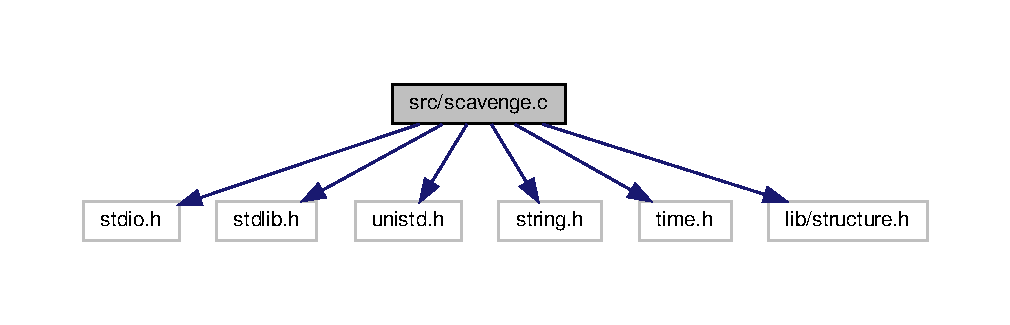
\includegraphics[width=350pt]{scavenge_8c__incl}
\end{center}
\end{figure}
\subsection*{Fonctions}
\begin{DoxyCompactItemize}
\item 
void \hyperlink{scavenge_8c_a2b60c717462304f30e1266e9a5a9d020}{generate\+\_\+items} (item\+\_\+t $\ast$Tab\+\_\+\+Items, int nb\+\_\+items\+\_\+available, perso\+\_\+t $\ast$player, categ\+\_\+hexa categ)
\begin{DoxyCompactList}\small\item\em Génère aléatoirement 0 à 5 items en prenant en compte le pourcentage de chance des items d\textquotesingle{}apparaître dans un type d\textquotesingle{}hexagone en particulier. \end{DoxyCompactList}\item 
void \hyperlink{scavenge_8c_aab16a4c396dce3479e9c0f8d7755c808}{scavenge} (cell\+\_\+t map\mbox{[}D\mbox{]}\mbox{[}D\mbox{]}, perso\+\_\+t $\ast$player, item\+\_\+t $\ast$Tab\+\_\+\+Items, int nb\+\_\+items\+\_\+available)
\begin{DoxyCompactList}\small\item\em Permet au joueur de fouiller l\textquotesingle{}hexagone sur lequel il se trouve pour récupérer des items. \end{DoxyCompactList}\end{DoxyCompactItemize}


\subsection{Description détaillée}
Fonctionnalité \+: fouiller l\textquotesingle{}hexagone pour récupérer des items. 

\begin{DoxyAuthor}{Auteur}
Mathilde Mottay, Anaïs Mottier, Clément Mainguy, Moustapha Tsamarayev 
\end{DoxyAuthor}
\begin{DoxyVersion}{Version}
1.\+0 
\end{DoxyVersion}
\begin{DoxyDate}{Date}
2020 
\end{DoxyDate}


\subsection{Documentation des fonctions}
\mbox{\Hypertarget{scavenge_8c_a2b60c717462304f30e1266e9a5a9d020}\label{scavenge_8c_a2b60c717462304f30e1266e9a5a9d020}} 
\index{scavenge.\+c@{scavenge.\+c}!generate\+\_\+items@{generate\+\_\+items}}
\index{generate\+\_\+items@{generate\+\_\+items}!scavenge.\+c@{scavenge.\+c}}
\subsubsection{\texorpdfstring{generate\+\_\+items()}{generate\_items()}}
{\footnotesize\ttfamily void generate\+\_\+items (\begin{DoxyParamCaption}\item[{item\+\_\+t $\ast$}]{Tab\+\_\+\+Items,  }\item[{int}]{nb\+\_\+items\+\_\+available,  }\item[{perso\+\_\+t $\ast$}]{player,  }\item[{categ\+\_\+hexa}]{categ }\end{DoxyParamCaption})}



Génère aléatoirement 0 à 5 items en prenant en compte le pourcentage de chance des items d\textquotesingle{}apparaître dans un type d\textquotesingle{}hexagone en particulier. 

Propose au joueur de récupérer les items générés 
\begin{DoxyParams}{Paramètres}
{\em item\+\_\+t} & $\ast$ Tab\+\_\+\+Items \\
\hline
{\em int} & nb\+\_\+items\+\_\+available \\
\hline
{\em perso\+\_\+t} & $\ast$ player \\
\hline
{\em categ\+\_\+hexa} & categ \\
\hline
\end{DoxyParams}
\begin{DoxyReturn}{Renvoie}
Rien 
\end{DoxyReturn}
\mbox{\Hypertarget{scavenge_8c_aab16a4c396dce3479e9c0f8d7755c808}\label{scavenge_8c_aab16a4c396dce3479e9c0f8d7755c808}} 
\index{scavenge.\+c@{scavenge.\+c}!scavenge@{scavenge}}
\index{scavenge@{scavenge}!scavenge.\+c@{scavenge.\+c}}
\subsubsection{\texorpdfstring{scavenge()}{scavenge()}}
{\footnotesize\ttfamily void scavenge (\begin{DoxyParamCaption}\item[{cell\+\_\+t}]{map\mbox{[}\+D\mbox{]}\mbox{[}\+D\mbox{]},  }\item[{perso\+\_\+t $\ast$}]{player,  }\item[{item\+\_\+t $\ast$}]{Tab\+\_\+\+Items,  }\item[{int}]{nb\+\_\+items\+\_\+available }\end{DoxyParamCaption})}



Permet au joueur de fouiller l\textquotesingle{}hexagone sur lequel il se trouve pour récupérer des items. 


\begin{DoxyParams}{Paramètres}
{\em cell\+\_\+t} & map\mbox{[}D\mbox{]}\mbox{[}D\mbox{]} \\
\hline
{\em perso\+\_\+t} & $\ast$ player \\
\hline
{\em item\+\_\+t} & $\ast$ Tab\+\_\+\+Items \\
\hline
{\em int} & nb\+\_\+items\+\_\+available \\
\hline
\end{DoxyParams}
\begin{DoxyReturn}{Renvoie}
Rien 
\end{DoxyReturn}

\hypertarget{turn_8c}{}\section{Référence du fichier src/turn.c}
\label{turn_8c}\index{src/turn.\+c@{src/turn.\+c}}


Fonctions relatives à un tour du jeu.  


{\ttfamily \#include $<$stdio.\+h$>$}\newline
{\ttfamily \#include $<$stdlib.\+h$>$}\newline
{\ttfamily \#include $<$string.\+h$>$}\newline
{\ttfamily \#include $<$time.\+h$>$}\newline
{\ttfamily \#include $<$unistd.\+h$>$}\newline
{\ttfamily \#include \char`\"{}lib/commun.\+h\char`\"{}}\newline
Graphe des dépendances par inclusion de turn.\+c\+:\nopagebreak
\begin{figure}[H]
\begin{center}
\leavevmode
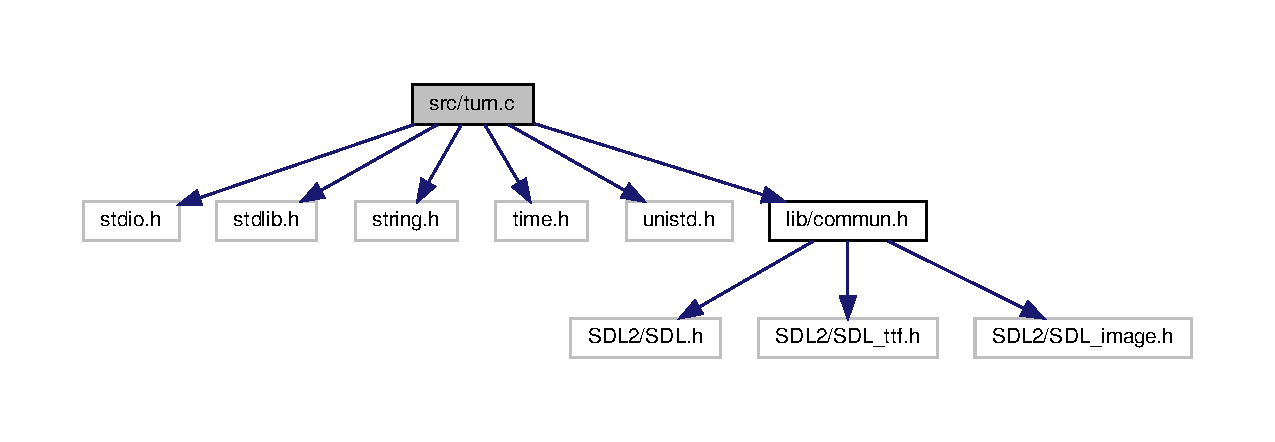
\includegraphics[width=350pt]{turn_8c__incl}
\end{center}
\end{figure}
\subsection*{Fonctions}
\begin{DoxyCompactItemize}
\item 
void \hyperlink{turn_8c_ab34814b4d8a3404f1d08ca212259c39b}{next\+\_\+turn} (\hyperlink{structperso__t}{perso\+\_\+t} $\ast$player)
\begin{DoxyCompactList}\small\item\em Calcule le nombre de points d’action récupérés à partir de la valeur des points d\textquotesingle{}énergie du joueur puis passe au tour suivant. \end{DoxyCompactList}\item 
void \hyperlink{turn_8c_a16623bb45a52000b8ec7b116aaa46173}{rest\+\_\+and\+\_\+heal} (\hyperlink{structperso__t}{perso\+\_\+t} $\ast$player)
\begin{DoxyCompactList}\small\item\em Permet au joueur de se reposer et récupérer des points de vie et points d\textquotesingle{}énergie (proportionnellement au nombre de points d\textquotesingle{}action) \end{DoxyCompactList}\end{DoxyCompactItemize}


\subsection{Description détaillée}
Fonctions relatives à un tour du jeu. 

\begin{DoxyAuthor}{Auteur}
Mathilde Mottay, Anaïs Mottier, Clément Mainguy, Moustapha Tsamarayev 
\end{DoxyAuthor}
\begin{DoxyVersion}{Version}
1.\+0 
\end{DoxyVersion}
\begin{DoxyDate}{Date}
2020 
\end{DoxyDate}


\subsection{Documentation des fonctions}
\mbox{\Hypertarget{turn_8c_ab34814b4d8a3404f1d08ca212259c39b}\label{turn_8c_ab34814b4d8a3404f1d08ca212259c39b}} 
\index{turn.\+c@{turn.\+c}!next\+\_\+turn@{next\+\_\+turn}}
\index{next\+\_\+turn@{next\+\_\+turn}!turn.\+c@{turn.\+c}}
\subsubsection{\texorpdfstring{next\+\_\+turn()}{next\_turn()}}
{\footnotesize\ttfamily void next\+\_\+turn (\begin{DoxyParamCaption}\item[{\hyperlink{structperso__t}{perso\+\_\+t} $\ast$}]{player }\end{DoxyParamCaption})}



Calcule le nombre de points d’action récupérés à partir de la valeur des points d\textquotesingle{}énergie du joueur puis passe au tour suivant. 


\begin{DoxyParams}{Paramètres}
{\em player} & Pointeur sur un objet de type \hyperlink{structperso__t}{perso\+\_\+t} correspondant au joueur \\
\hline
\end{DoxyParams}
\begin{DoxyReturn}{Renvoie}
Rien 
\end{DoxyReturn}
\mbox{\Hypertarget{turn_8c_a16623bb45a52000b8ec7b116aaa46173}\label{turn_8c_a16623bb45a52000b8ec7b116aaa46173}} 
\index{turn.\+c@{turn.\+c}!rest\+\_\+and\+\_\+heal@{rest\+\_\+and\+\_\+heal}}
\index{rest\+\_\+and\+\_\+heal@{rest\+\_\+and\+\_\+heal}!turn.\+c@{turn.\+c}}
\subsubsection{\texorpdfstring{rest\+\_\+and\+\_\+heal()}{rest\_and\_heal()}}
{\footnotesize\ttfamily void rest\+\_\+and\+\_\+heal (\begin{DoxyParamCaption}\item[{\hyperlink{structperso__t}{perso\+\_\+t} $\ast$}]{player }\end{DoxyParamCaption})}



Permet au joueur de se reposer et récupérer des points de vie et points d\textquotesingle{}énergie (proportionnellement au nombre de points d\textquotesingle{}action) 


\begin{DoxyParams}{Paramètres}
{\em player} & Pointeur sur un objet de type \hyperlink{structperso__t}{perso\+\_\+t} correspondant au joueur \\
\hline
\end{DoxyParams}
\begin{DoxyReturn}{Renvoie}
Rien 
\end{DoxyReturn}

\hypertarget{world__generation_8c}{}\section{Référence du fichier src/world\+\_\+generation.c}
\label{world__generation_8c}\index{src/world\+\_\+generation.\+c@{src/world\+\_\+generation.\+c}}


Génération de la carte.  


{\ttfamily \#include $<$stdio.\+h$>$}\newline
{\ttfamily \#include $<$stdlib.\+h$>$}\newline
{\ttfamily \#include $<$time.\+h$>$}\newline
{\ttfamily \#include \char`\"{}lib/commun.\+h\char`\"{}}\newline
Graphe des dépendances par inclusion de world\+\_\+generation.\+c\+:\nopagebreak
\begin{figure}[H]
\begin{center}
\leavevmode
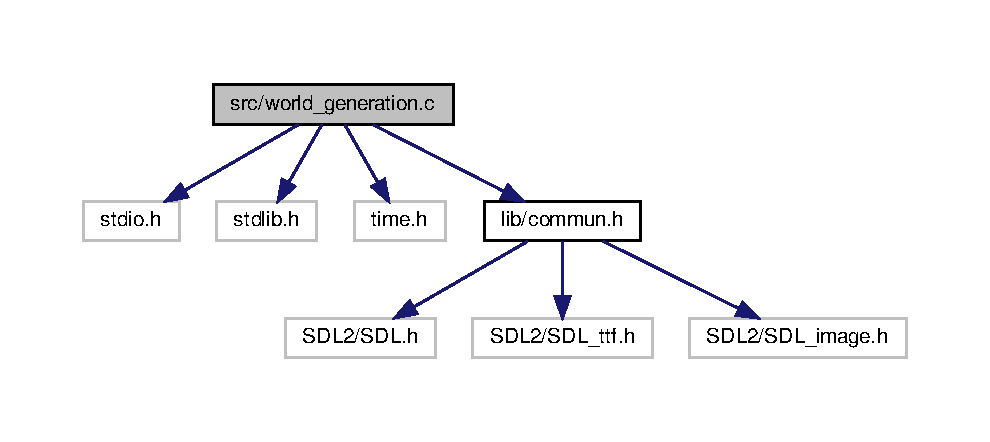
\includegraphics[width=350pt]{world__generation_8c__incl}
\end{center}
\end{figure}
\subsection*{Fonctions}
\begin{DoxyCompactItemize}
\item 
void \hyperlink{world__generation_8c_a719ffd0c2cb14a6236922fac92933adb}{afficher\+\_\+type\+\_\+categ\+\_\+hexa} (\hyperlink{structcell__t}{cell\+\_\+t} map\mbox{[}\hyperlink{commun_8h_af316c33cc298530f245e8b55330e86b5}{D}\mbox{]}\mbox{[}\hyperlink{commun_8h_af316c33cc298530f245e8b55330e86b5}{D}\mbox{]}, int l, int c)
\begin{DoxyCompactList}\small\item\em Affiche le type et la catégorie de l\textquotesingle{}hexagone de la carte dont les coordonnées sont passées en paramètres. \end{DoxyCompactList}\item 
void \hyperlink{world__generation_8c_acc7e7b34903dd75f8563deda4e525f39}{informations\+\_\+map} (\hyperlink{structcell__t}{cell\+\_\+t} map\mbox{[}\hyperlink{commun_8h_af316c33cc298530f245e8b55330e86b5}{D}\mbox{]}\mbox{[}\hyperlink{commun_8h_af316c33cc298530f245e8b55330e86b5}{D}\mbox{]})
\begin{DoxyCompactList}\small\item\em Affiche les informations de la carte. \end{DoxyCompactList}\item 
void \hyperlink{world__generation_8c_a8ab726a1d0a373a9b5e762ae74e6af55}{init\+\_\+border} (\hyperlink{structcell__t}{cell\+\_\+t} map\mbox{[}\hyperlink{commun_8h_af316c33cc298530f245e8b55330e86b5}{D}\mbox{]}\mbox{[}\hyperlink{commun_8h_af316c33cc298530f245e8b55330e86b5}{D}\mbox{]})
\begin{DoxyCompactList}\small\item\em Initialise les contours de la map. \end{DoxyCompactList}\item 
void \hyperlink{world__generation_8c_ad5c57c2778c1e760fad1f9d17f97f0d7}{topup} (\hyperlink{structcell__t}{cell\+\_\+t} map\mbox{[}\hyperlink{commun_8h_af316c33cc298530f245e8b55330e86b5}{D}\mbox{]}\mbox{[}\hyperlink{commun_8h_af316c33cc298530f245e8b55330e86b5}{D}\mbox{]}, int quest\+\_\+map\mbox{[}6\mbox{]}\mbox{[}2\mbox{]})
\begin{DoxyCompactList}\small\item\em Crée un nombre déterminé d’hexagones indispensables pour la carte (comme camp militaire/bandit par exemple) sur des coordonnées aléatoires. \end{DoxyCompactList}\item 
int \hyperlink{world__generation_8c_a610b48bca978adae918ba8c023c49571}{spawntype} (int l, int c, \hyperlink{structcell__t}{cell\+\_\+t} map\mbox{[}\hyperlink{commun_8h_af316c33cc298530f245e8b55330e86b5}{D}\mbox{]}\mbox{[}\hyperlink{commun_8h_af316c33cc298530f245e8b55330e86b5}{D}\mbox{]})
\begin{DoxyCompactList}\small\item\em Compte le nombre d\textquotesingle{}hexagones-\/voisins similaires et selon ce nombre, après des calculs de probabilité, renvoie le type d’hexagone qui sera créé sur les coordonnées passées en paramètre. \end{DoxyCompactList}\item 
int \hyperlink{world__generation_8c_a7a53fec4d8948be421914833d195af0b}{categ\+\_\+switch} (int input)
\begin{DoxyCompactList}\small\item\em Donne la catégorie de l\textquotesingle{}hexagone passé en paramètre. \end{DoxyCompactList}\item 
void \hyperlink{world__generation_8c_a7a0d3066e88d63d7fb191f7a810e1d3d}{nextgen} (\hyperlink{structcell__t}{cell\+\_\+t} map\mbox{[}\hyperlink{commun_8h_af316c33cc298530f245e8b55330e86b5}{D}\mbox{]}\mbox{[}\hyperlink{commun_8h_af316c33cc298530f245e8b55330e86b5}{D}\mbox{]})
\begin{DoxyCompactList}\small\item\em Parcours la matrice de la carte passée en paramètre et fait appel à \hyperlink{world__generation_8c_a610b48bca978adae918ba8c023c49571}{spawntype} pour calculer le type d’hexagone qui va apparaître dans la cellule courante. \end{DoxyCompactList}\item 
int \hyperlink{world__generation_8c_a0f6eb129fcf00e592e708ad17e0a65ac}{coordonnees\+\_\+valides} (int l, int c)
\begin{DoxyCompactList}\small\item\em Vérifie si les coordonnées sont valides. \end{DoxyCompactList}\item 
void \hyperlink{world__generation_8c_ac44e2e3723ce06a3660665d0adc23079}{portable\+\_\+switch} (int i, int j, \hyperlink{structcell__t}{cell\+\_\+t} map\mbox{[}\hyperlink{commun_8h_af316c33cc298530f245e8b55330e86b5}{D}\mbox{]}\mbox{[}\hyperlink{commun_8h_af316c33cc298530f245e8b55330e86b5}{D}\mbox{]})
\begin{DoxyCompactList}\small\item\em Affiche le code de la cellule. \end{DoxyCompactList}\item 
void \hyperlink{world__generation_8c_a3bc1a448a2edbe81a579122cd06467ac}{display\+\_\+\+T\+E\+XT} (int l, int c, \hyperlink{structcell__t}{cell\+\_\+t} map\mbox{[}\hyperlink{commun_8h_af316c33cc298530f245e8b55330e86b5}{D}\mbox{]}\mbox{[}\hyperlink{commun_8h_af316c33cc298530f245e8b55330e86b5}{D}\mbox{]})
\begin{DoxyCompactList}\small\item\em Affiche la map en version texte avec la légende. \end{DoxyCompactList}\item 
void \hyperlink{world__generation_8c_ab4a79a51d27f37c50336cf450fc770cf}{init\+\_\+base} (\hyperlink{structcell__t}{cell\+\_\+t} map\mbox{[}\hyperlink{commun_8h_af316c33cc298530f245e8b55330e86b5}{D}\mbox{]}\mbox{[}\hyperlink{commun_8h_af316c33cc298530f245e8b55330e86b5}{D}\mbox{]})
\begin{DoxyCompactList}\small\item\em Initialise la base de la carte. \end{DoxyCompactList}\item 
void \hyperlink{world__generation_8c_a6f2790bca8e59fe3b65ca808f1500821}{count} (const \hyperlink{structcell__t}{cell\+\_\+t} map\mbox{[}\hyperlink{commun_8h_af316c33cc298530f245e8b55330e86b5}{D}\mbox{]}\mbox{[}\hyperlink{commun_8h_af316c33cc298530f245e8b55330e86b5}{D}\mbox{]})
\begin{DoxyCompactList}\small\item\em Compte le nombre d\textquotesingle{}occurence de chaque type de cellule (outil de test) \end{DoxyCompactList}\item 
void \hyperlink{world__generation_8c_ae2a948ed1b1ff33428390c62f9371aef}{encounter\+\_\+init} (\hyperlink{structcell__t}{cell\+\_\+t} map\mbox{[}\hyperlink{commun_8h_af316c33cc298530f245e8b55330e86b5}{D}\mbox{]}\mbox{[}\hyperlink{commun_8h_af316c33cc298530f245e8b55330e86b5}{D}\mbox{]})
\begin{DoxyCompactList}\small\item\em Initialise les positions des combats sur la carte. \end{DoxyCompactList}\item 
void \hyperlink{world__generation_8c_a61aa43ceaa893c5807b45cd54fd140e8}{quest\+\_\+init} (\hyperlink{structcell__t}{cell\+\_\+t} map\mbox{[}\hyperlink{commun_8h_af316c33cc298530f245e8b55330e86b5}{D}\mbox{]}\mbox{[}\hyperlink{commun_8h_af316c33cc298530f245e8b55330e86b5}{D}\mbox{]}, int quest\+\_\+map\mbox{[}6\mbox{]}\mbox{[}2\mbox{]})
\begin{DoxyCompactList}\small\item\em Initialise les quêtes (quest\+\_\+id) sur la carte. \end{DoxyCompactList}\item 
void \hyperlink{world__generation_8c_a309363eb6ec82b7f53f004bbd01c21c4}{map\+\_\+init} (\hyperlink{structcell__t}{cell\+\_\+t} map\mbox{[}\hyperlink{commun_8h_af316c33cc298530f245e8b55330e86b5}{D}\mbox{]}\mbox{[}\hyperlink{commun_8h_af316c33cc298530f245e8b55330e86b5}{D}\mbox{]}, int quest\+\_\+map\mbox{[}6\mbox{]}\mbox{[}2\mbox{]})
\begin{DoxyCompactList}\small\item\em Initialise la carte au début de chaque partie. \end{DoxyCompactList}\end{DoxyCompactItemize}


\subsection{Description détaillée}
Génération de la carte. 

\begin{DoxyAuthor}{Auteur}
Mathilde Mottay, Anaïs Mottier, Clément Mainguy, Moustapha Tsamarayev 
\end{DoxyAuthor}
\begin{DoxyVersion}{Version}
1.\+0 
\end{DoxyVersion}
\begin{DoxyDate}{Date}
2020 
\end{DoxyDate}


\subsection{Documentation des fonctions}
\mbox{\Hypertarget{world__generation_8c_a719ffd0c2cb14a6236922fac92933adb}\label{world__generation_8c_a719ffd0c2cb14a6236922fac92933adb}} 
\index{world\+\_\+generation.\+c@{world\+\_\+generation.\+c}!afficher\+\_\+type\+\_\+categ\+\_\+hexa@{afficher\+\_\+type\+\_\+categ\+\_\+hexa}}
\index{afficher\+\_\+type\+\_\+categ\+\_\+hexa@{afficher\+\_\+type\+\_\+categ\+\_\+hexa}!world\+\_\+generation.\+c@{world\+\_\+generation.\+c}}
\subsubsection{\texorpdfstring{afficher\+\_\+type\+\_\+categ\+\_\+hexa()}{afficher\_type\_categ\_hexa()}}
{\footnotesize\ttfamily void afficher\+\_\+type\+\_\+categ\+\_\+hexa (\begin{DoxyParamCaption}\item[{\hyperlink{structcell__t}{cell\+\_\+t}}]{map\mbox{[}\+D\mbox{]}\mbox{[}\+D\mbox{]},  }\item[{int}]{l,  }\item[{int}]{c }\end{DoxyParamCaption})}



Affiche le type et la catégorie de l\textquotesingle{}hexagone de la carte dont les coordonnées sont passées en paramètres. 


\begin{DoxyParams}{Paramètres}
{\em map\mbox{[}\+D\mbox{]}\mbox{[}\+D\mbox{]}} & Matrice de la carte \\
\hline
{\em l} & Coordonnée ligne de l\textquotesingle{}hexagone qu\textquotesingle{}on souhaite afficher \\
\hline
{\em c} & Coordonnée colonne de l\textquotesingle{}hexagone qu\textquotesingle{}on souhaite afficher \\
\hline
\end{DoxyParams}
\begin{DoxyReturn}{Renvoie}
Rien 
\end{DoxyReturn}
\mbox{\Hypertarget{world__generation_8c_a7a53fec4d8948be421914833d195af0b}\label{world__generation_8c_a7a53fec4d8948be421914833d195af0b}} 
\index{world\+\_\+generation.\+c@{world\+\_\+generation.\+c}!categ\+\_\+switch@{categ\+\_\+switch}}
\index{categ\+\_\+switch@{categ\+\_\+switch}!world\+\_\+generation.\+c@{world\+\_\+generation.\+c}}
\subsubsection{\texorpdfstring{categ\+\_\+switch()}{categ\_switch()}}
{\footnotesize\ttfamily int categ\+\_\+switch (\begin{DoxyParamCaption}\item[{int}]{input }\end{DoxyParamCaption})}



Donne la catégorie de l\textquotesingle{}hexagone passé en paramètre. 


\begin{DoxyParams}{Paramètres}
{\em input} & Type d\textquotesingle{}hexagone \\
\hline
\end{DoxyParams}
\begin{DoxyReturn}{Renvoie}
Retourne un {\itshape int} correspondant à la catégorie de l\textquotesingle{}hexagone 
\end{DoxyReturn}
\mbox{\Hypertarget{world__generation_8c_a0f6eb129fcf00e592e708ad17e0a65ac}\label{world__generation_8c_a0f6eb129fcf00e592e708ad17e0a65ac}} 
\index{world\+\_\+generation.\+c@{world\+\_\+generation.\+c}!coordonnees\+\_\+valides@{coordonnees\+\_\+valides}}
\index{coordonnees\+\_\+valides@{coordonnees\+\_\+valides}!world\+\_\+generation.\+c@{world\+\_\+generation.\+c}}
\subsubsection{\texorpdfstring{coordonnees\+\_\+valides()}{coordonnees\_valides()}}
{\footnotesize\ttfamily int coordonnees\+\_\+valides (\begin{DoxyParamCaption}\item[{int}]{l,  }\item[{int}]{c }\end{DoxyParamCaption})}



Vérifie si les coordonnées sont valides. 


\begin{DoxyParams}{Paramètres}
{\em l} & Coordonnée ligne \\
\hline
{\em c} & Coordonnée colonne \\
\hline
\end{DoxyParams}
\begin{DoxyReturn}{Renvoie}
Retourne un {\itshape int} \+: 1 si les coordonnées sont valides, 0 si non 
\end{DoxyReturn}
\mbox{\Hypertarget{world__generation_8c_a6f2790bca8e59fe3b65ca808f1500821}\label{world__generation_8c_a6f2790bca8e59fe3b65ca808f1500821}} 
\index{world\+\_\+generation.\+c@{world\+\_\+generation.\+c}!count@{count}}
\index{count@{count}!world\+\_\+generation.\+c@{world\+\_\+generation.\+c}}
\subsubsection{\texorpdfstring{count()}{count()}}
{\footnotesize\ttfamily void count (\begin{DoxyParamCaption}\item[{const \hyperlink{structcell__t}{cell\+\_\+t}}]{map\mbox{[}\+D\mbox{]}\mbox{[}\+D\mbox{]} }\end{DoxyParamCaption})}



Compte le nombre d\textquotesingle{}occurence de chaque type de cellule (outil de test) 


\begin{DoxyParams}{Paramètres}
{\em map\mbox{[}\+D\mbox{]}\mbox{[}\+D\mbox{]}} & Matrice de la carte \\
\hline
\end{DoxyParams}
\begin{DoxyReturn}{Renvoie}
Rien 
\end{DoxyReturn}
\mbox{\Hypertarget{world__generation_8c_a3bc1a448a2edbe81a579122cd06467ac}\label{world__generation_8c_a3bc1a448a2edbe81a579122cd06467ac}} 
\index{world\+\_\+generation.\+c@{world\+\_\+generation.\+c}!display\+\_\+\+T\+E\+XT@{display\+\_\+\+T\+E\+XT}}
\index{display\+\_\+\+T\+E\+XT@{display\+\_\+\+T\+E\+XT}!world\+\_\+generation.\+c@{world\+\_\+generation.\+c}}
\subsubsection{\texorpdfstring{display\+\_\+\+T\+E\+X\+T()}{display\_TEXT()}}
{\footnotesize\ttfamily void display\+\_\+\+T\+E\+XT (\begin{DoxyParamCaption}\item[{int}]{l,  }\item[{int}]{c,  }\item[{\hyperlink{structcell__t}{cell\+\_\+t}}]{map\mbox{[}\+D\mbox{]}\mbox{[}\+D\mbox{]} }\end{DoxyParamCaption})}



Affiche la map en version texte avec la légende. 


\begin{DoxyParams}{Paramètres}
{\em l} & Coordonnée ligne \\
\hline
{\em c} & Coordonnée colonne \\
\hline
{\em map\mbox{[}\+D\mbox{]}\mbox{[}\+D\mbox{]}} & Matrice de la carte \\
\hline
\end{DoxyParams}
\begin{DoxyReturn}{Renvoie}
Rien 
\end{DoxyReturn}
\mbox{\Hypertarget{world__generation_8c_ae2a948ed1b1ff33428390c62f9371aef}\label{world__generation_8c_ae2a948ed1b1ff33428390c62f9371aef}} 
\index{world\+\_\+generation.\+c@{world\+\_\+generation.\+c}!encounter\+\_\+init@{encounter\+\_\+init}}
\index{encounter\+\_\+init@{encounter\+\_\+init}!world\+\_\+generation.\+c@{world\+\_\+generation.\+c}}
\subsubsection{\texorpdfstring{encounter\+\_\+init()}{encounter\_init()}}
{\footnotesize\ttfamily void encounter\+\_\+init (\begin{DoxyParamCaption}\item[{\hyperlink{structcell__t}{cell\+\_\+t}}]{map\mbox{[}\+D\mbox{]}\mbox{[}\+D\mbox{]} }\end{DoxyParamCaption})}



Initialise les positions des combats sur la carte. 


\begin{DoxyParams}{Paramètres}
{\em map\mbox{[}\+D\mbox{]}\mbox{[}\+D\mbox{]}} & Matrice de la carte \\
\hline
\end{DoxyParams}
\begin{DoxyReturn}{Renvoie}
Rien 
\end{DoxyReturn}
\mbox{\Hypertarget{world__generation_8c_acc7e7b34903dd75f8563deda4e525f39}\label{world__generation_8c_acc7e7b34903dd75f8563deda4e525f39}} 
\index{world\+\_\+generation.\+c@{world\+\_\+generation.\+c}!informations\+\_\+map@{informations\+\_\+map}}
\index{informations\+\_\+map@{informations\+\_\+map}!world\+\_\+generation.\+c@{world\+\_\+generation.\+c}}
\subsubsection{\texorpdfstring{informations\+\_\+map()}{informations\_map()}}
{\footnotesize\ttfamily void informations\+\_\+map (\begin{DoxyParamCaption}\item[{\hyperlink{structcell__t}{cell\+\_\+t}}]{map\mbox{[}\+D\mbox{]}\mbox{[}\+D\mbox{]} }\end{DoxyParamCaption})}



Affiche les informations de la carte. 


\begin{DoxyParams}{Paramètres}
{\em map\mbox{[}\+D\mbox{]}\mbox{[}\+D\mbox{]}} & Matrice de la carte \\
\hline
\end{DoxyParams}
\begin{DoxyReturn}{Renvoie}
Rien 
\end{DoxyReturn}
\mbox{\Hypertarget{world__generation_8c_ab4a79a51d27f37c50336cf450fc770cf}\label{world__generation_8c_ab4a79a51d27f37c50336cf450fc770cf}} 
\index{world\+\_\+generation.\+c@{world\+\_\+generation.\+c}!init\+\_\+base@{init\+\_\+base}}
\index{init\+\_\+base@{init\+\_\+base}!world\+\_\+generation.\+c@{world\+\_\+generation.\+c}}
\subsubsection{\texorpdfstring{init\+\_\+base()}{init\_base()}}
{\footnotesize\ttfamily void init\+\_\+base (\begin{DoxyParamCaption}\item[{\hyperlink{structcell__t}{cell\+\_\+t}}]{map\mbox{[}\+D\mbox{]}\mbox{[}\+D\mbox{]} }\end{DoxyParamCaption})}



Initialise la base de la carte. 

La carte est initialisée par des hexagones de type prairie (catégorie nature), sans combat, sans quête et sans hexagones fouillés. 
\begin{DoxyParams}{Paramètres}
{\em map\mbox{[}\+D\mbox{]}\mbox{[}\+D\mbox{]}} & Matrice de la carte \\
\hline
\end{DoxyParams}
\begin{DoxyReturn}{Renvoie}
Rien 
\end{DoxyReturn}
\mbox{\Hypertarget{world__generation_8c_a8ab726a1d0a373a9b5e762ae74e6af55}\label{world__generation_8c_a8ab726a1d0a373a9b5e762ae74e6af55}} 
\index{world\+\_\+generation.\+c@{world\+\_\+generation.\+c}!init\+\_\+border@{init\+\_\+border}}
\index{init\+\_\+border@{init\+\_\+border}!world\+\_\+generation.\+c@{world\+\_\+generation.\+c}}
\subsubsection{\texorpdfstring{init\+\_\+border()}{init\_border()}}
{\footnotesize\ttfamily void init\+\_\+border (\begin{DoxyParamCaption}\item[{\hyperlink{structcell__t}{cell\+\_\+t}}]{map\mbox{[}\+D\mbox{]}\mbox{[}\+D\mbox{]} }\end{DoxyParamCaption})}



Initialise les contours de la map. 


\begin{DoxyParams}{Paramètres}
{\em map\mbox{[}\+D\mbox{]}\mbox{[}\+D\mbox{]}} & Matrice de la carte \\
\hline
\end{DoxyParams}
\begin{DoxyReturn}{Renvoie}
Rien 
\end{DoxyReturn}
\mbox{\Hypertarget{world__generation_8c_a309363eb6ec82b7f53f004bbd01c21c4}\label{world__generation_8c_a309363eb6ec82b7f53f004bbd01c21c4}} 
\index{world\+\_\+generation.\+c@{world\+\_\+generation.\+c}!map\+\_\+init@{map\+\_\+init}}
\index{map\+\_\+init@{map\+\_\+init}!world\+\_\+generation.\+c@{world\+\_\+generation.\+c}}
\subsubsection{\texorpdfstring{map\+\_\+init()}{map\_init()}}
{\footnotesize\ttfamily void map\+\_\+init (\begin{DoxyParamCaption}\item[{\hyperlink{structcell__t}{cell\+\_\+t}}]{map\mbox{[}\+D\mbox{]}\mbox{[}\+D\mbox{]},  }\item[{int}]{quest\+\_\+map\mbox{[}6\mbox{]}\mbox{[}2\mbox{]} }\end{DoxyParamCaption})}



Initialise la carte au début de chaque partie. 


\begin{DoxyParams}{Paramètres}
{\em map\mbox{[}\+D\mbox{]}\mbox{[}\+D\mbox{]}} & Matrice de la carte \\
\hline
{\em quest\+\_\+map\mbox{[}6\mbox{]}\mbox{[}2\mbox{]}} & Matrice des coordonnées des quêtes \\
\hline
{\em player} & Joueur \\
\hline
\end{DoxyParams}
\begin{DoxyReturn}{Renvoie}
Rien 
\end{DoxyReturn}
\mbox{\Hypertarget{world__generation_8c_a7a0d3066e88d63d7fb191f7a810e1d3d}\label{world__generation_8c_a7a0d3066e88d63d7fb191f7a810e1d3d}} 
\index{world\+\_\+generation.\+c@{world\+\_\+generation.\+c}!nextgen@{nextgen}}
\index{nextgen@{nextgen}!world\+\_\+generation.\+c@{world\+\_\+generation.\+c}}
\subsubsection{\texorpdfstring{nextgen()}{nextgen()}}
{\footnotesize\ttfamily void nextgen (\begin{DoxyParamCaption}\item[{\hyperlink{structcell__t}{cell\+\_\+t}}]{map\mbox{[}\+D\mbox{]}\mbox{[}\+D\mbox{]} }\end{DoxyParamCaption})}



Parcours la matrice de la carte passée en paramètre et fait appel à \hyperlink{world__generation_8c_a610b48bca978adae918ba8c023c49571}{spawntype} pour calculer le type d’hexagone qui va apparaître dans la cellule courante. 


\begin{DoxyParams}{Paramètres}
{\em map\mbox{[}\+D\mbox{]}\mbox{[}\+D\mbox{]}} & Matrice de la carte \\
\hline
\end{DoxyParams}
\begin{DoxyReturn}{Renvoie}
Rien 
\end{DoxyReturn}
\mbox{\Hypertarget{world__generation_8c_ac44e2e3723ce06a3660665d0adc23079}\label{world__generation_8c_ac44e2e3723ce06a3660665d0adc23079}} 
\index{world\+\_\+generation.\+c@{world\+\_\+generation.\+c}!portable\+\_\+switch@{portable\+\_\+switch}}
\index{portable\+\_\+switch@{portable\+\_\+switch}!world\+\_\+generation.\+c@{world\+\_\+generation.\+c}}
\subsubsection{\texorpdfstring{portable\+\_\+switch()}{portable\_switch()}}
{\footnotesize\ttfamily void portable\+\_\+switch (\begin{DoxyParamCaption}\item[{int}]{i,  }\item[{int}]{j,  }\item[{\hyperlink{structcell__t}{cell\+\_\+t}}]{map\mbox{[}\+D\mbox{]}\mbox{[}\+D\mbox{]} }\end{DoxyParamCaption})}



Affiche le code de la cellule. 

Cette fonction a été créée pour éviter de refaire le switch dans différentes fonctions d\textquotesingle{}affichage. 
\begin{DoxyParams}{Paramètres}
{\em i} & Coordonnée ligne \\
\hline
{\em j} & Coordonnée colonne \\
\hline
{\em map\mbox{[}\+D\mbox{]}\mbox{[}\+D\mbox{]}} & Matrice de la carte \\
\hline
\end{DoxyParams}
\begin{DoxyReturn}{Renvoie}
Rien 
\end{DoxyReturn}
\mbox{\Hypertarget{world__generation_8c_a61aa43ceaa893c5807b45cd54fd140e8}\label{world__generation_8c_a61aa43ceaa893c5807b45cd54fd140e8}} 
\index{world\+\_\+generation.\+c@{world\+\_\+generation.\+c}!quest\+\_\+init@{quest\+\_\+init}}
\index{quest\+\_\+init@{quest\+\_\+init}!world\+\_\+generation.\+c@{world\+\_\+generation.\+c}}
\subsubsection{\texorpdfstring{quest\+\_\+init()}{quest\_init()}}
{\footnotesize\ttfamily void quest\+\_\+init (\begin{DoxyParamCaption}\item[{\hyperlink{structcell__t}{cell\+\_\+t}}]{map\mbox{[}\+D\mbox{]}\mbox{[}\+D\mbox{]},  }\item[{int}]{quest\+\_\+map\mbox{[}6\mbox{]}\mbox{[}2\mbox{]} }\end{DoxyParamCaption})}



Initialise les quêtes (quest\+\_\+id) sur la carte. 

Les quêtes sont placées aléatoirement sur la carte. 
\begin{DoxyParams}{Paramètres}
{\em map\mbox{[}\+D\mbox{]}\mbox{[}\+D\mbox{]}} & Matrice de la carte \\
\hline
{\em quest\+\_\+map\mbox{[}6\mbox{]}\mbox{[}2\mbox{]}} & Matrice des coordonnées des quêtes \\
\hline
\end{DoxyParams}
\begin{DoxyReturn}{Renvoie}
Rien 
\end{DoxyReturn}
\mbox{\Hypertarget{world__generation_8c_a610b48bca978adae918ba8c023c49571}\label{world__generation_8c_a610b48bca978adae918ba8c023c49571}} 
\index{world\+\_\+generation.\+c@{world\+\_\+generation.\+c}!spawntype@{spawntype}}
\index{spawntype@{spawntype}!world\+\_\+generation.\+c@{world\+\_\+generation.\+c}}
\subsubsection{\texorpdfstring{spawntype()}{spawntype()}}
{\footnotesize\ttfamily int spawntype (\begin{DoxyParamCaption}\item[{int}]{l,  }\item[{int}]{c,  }\item[{\hyperlink{structcell__t}{cell\+\_\+t}}]{map\mbox{[}\+D\mbox{]}\mbox{[}\+D\mbox{]} }\end{DoxyParamCaption})}



Compte le nombre d\textquotesingle{}hexagones-\/voisins similaires et selon ce nombre, après des calculs de probabilité, renvoie le type d’hexagone qui sera créé sur les coordonnées passées en paramètre. 


\begin{DoxyParams}{Paramètres}
{\em l} & Coordonnée ligne \\
\hline
{\em c} & Coordonnée colonne \\
\hline
{\em map\mbox{[}\+D\mbox{]}\mbox{[}\+D\mbox{]}} & Matrice de la carte \\
\hline
\end{DoxyParams}
\begin{DoxyReturn}{Renvoie}
Retourne un {\itshape int} \+: le type de l\textquotesingle{}hexagone qui va être créé 
\end{DoxyReturn}
\mbox{\Hypertarget{world__generation_8c_ad5c57c2778c1e760fad1f9d17f97f0d7}\label{world__generation_8c_ad5c57c2778c1e760fad1f9d17f97f0d7}} 
\index{world\+\_\+generation.\+c@{world\+\_\+generation.\+c}!topup@{topup}}
\index{topup@{topup}!world\+\_\+generation.\+c@{world\+\_\+generation.\+c}}
\subsubsection{\texorpdfstring{topup()}{topup()}}
{\footnotesize\ttfamily void topup (\begin{DoxyParamCaption}\item[{\hyperlink{structcell__t}{cell\+\_\+t}}]{map\mbox{[}\+D\mbox{]}\mbox{[}\+D\mbox{]},  }\item[{int}]{quest\+\_\+map\mbox{[}6\mbox{]}\mbox{[}2\mbox{]} }\end{DoxyParamCaption})}



Crée un nombre déterminé d’hexagones indispensables pour la carte (comme camp militaire/bandit par exemple) sur des coordonnées aléatoires. 


\begin{DoxyParams}{Paramètres}
{\em map\mbox{[}\+D\mbox{]}\mbox{[}\+D\mbox{]}} & Matrice de la carte \\
\hline
{\em quest\+\_\+map\mbox{[}6\mbox{]}\mbox{[}2\mbox{]}} & Matrice des coordonnées des quêtes \\
\hline
\end{DoxyParams}
\begin{DoxyReturn}{Renvoie}
Rien 
\end{DoxyReturn}

%--- End generated contents ---

% Index
\backmatter
\newpage
\phantomsection
\clearemptydoublepage
\addcontentsline{toc}{chapter}{Index}
\printindex

\end{document}
